\documentclass[10pt]{article}
%\documentclass[10pt,landscape]{article}
\usepackage[ngerman]{babel}
\usepackage{multicol}
\usepackage{calc}
\usepackage{ifthen}
\usepackage[]{geometry}
%\usepackage[landscape]{geometry}
\usepackage{amsmath,amsthm,amsfonts,amssymb}
\usepackage{color,graphicx,overpic}
\usepackage{hyperref}
\usepackage{listings}
\usepackage[compact]{titlesec} %less space for headers
\usepackage{mdwlist} %less space for lists
\usepackage[dvipsnames]{xcolor}

\pdfinfo{
    /Title (Programmierparadigmen - Cheatsheet)
    /Creator (TeX)
    /Producer (pdfTeX 1.40.0)
    /Author (Robert Jeutter)
    /Subject ()
}

% This sets page margins to .5 inch if using letter paper, and to 1cm
% if using A4 paper. (This probably isn't strictly necessary.)
% If using another size paper, use default 1cm margins.
\ifthenelse{\lengthtest { \paperwidth = 11in}}
    { \geometry{top=.5in,left=.5in,right=.5in,bottom=.5in} }
    {\ifthenelse{ \lengthtest{ \paperwidth = 297mm}}
        {\geometry{top=1cm,left=1cm,right=1cm,bottom=1cm} }
        {\geometry{top=1cm,left=1cm,right=1cm,bottom=1cm} }
    }


    \definecolor{commentsColor}{rgb}{0.497495, 0.497587, 0.497464}
    \definecolor{keywordsColor}{rgb}{0.000000, 0.000000, 0.635294}
    \definecolor{stringColor}{rgb}{0.558215, 0.000000, 0.135316}
    \lstset{
      backgroundcolor=\color{white},   % choose the background color; you must add \usepackage{color} or \usepackage{xcolor}
      basicstyle=\ttfamily,        % the size of the fonts that are used for the code
      breakatwhitespace=false,         % sets if automatic breaks should only happen at whitespace
      breaklines=true,                 % sets automatic line breaking
      captionpos=b,                    % sets the caption-position to bottom
      commentstyle=\color{commentsColor}\textit,    % comment style
      deletekeywords={...},            % if you want to delete keywords from the given language
      escapeinside={\%*}{*)},          % if you want to add LaTeX within your code
      extendedchars=true,              % lets you use non-ASCII characters; for 8-bits encodings only, does not work with UTF-8
      frame=tb,	                   	   % adds a frame around the code
      keepspaces=true,                 % keeps spaces in text, useful for keeping indentation of code (possibly needs columns=flexible)
      keywordstyle=\color{keywordsColor}\bfseries,       % keyword style
      language=Python,                 % the language of the code (can be overrided per snippet)
      otherkeywords={*,...},           % if you want to add more keywords to the set
      numbers=left,                    % where to put the line-numbers; possible values are (none, left, right)
      numbersep=5pt,                   % how far the line-numbers are from the code
      numberstyle=\tiny\color{commentsColor}, % the style that is used for the line-numbers
      rulecolor=\color{black},         % if not set, the frame-color may be changed on line-breaks within not-black text (e.g. comments (green here))
      showspaces=false,                % show spaces everywhere adding particular underscores; it overrides 'showstringspaces'
      showstringspaces=false,          % underline spaces within strings only
      showtabs=false,                  % show tabs within strings adding particular underscores
      stepnumber=1,                    % the step between two line-numbers. If it's 1, each line will be numbered
      stringstyle=\color{stringColor}, % string literal style
      tabsize=2,	                   % sets default tabsize to 2 spaces
      title=\lstname,                  % show the filename of files included with \lstinputlisting; also try caption instead of title
      columns=fixed,                    % Using fixed column width (for e.g. nice alignment)
      %identifierstyle=\color{red},
      literate=
        {Ö}{{\"O}}1
        {Ä}{{\"A}}1
        {Ü}{{\"U}}1
        {ß}{{\ss}}1
        {ü}{{\"u}}1
        {ä}{{\"a}}1
        {ö}{{\"o}}1
    }
% Turn off header and footer
\pagestyle{empty}

% Redefine section commands to use less space
\makeatletter
\renewcommand{\section}{\@startsection{section}{1}{0mm}%
                                {-1ex plus -.5ex minus -.2ex}%
                                {0.5ex plus .2ex}%x
                                {\normalfont\large\bfseries}}
\renewcommand{\subsection}{\@startsection{subsection}{2}{0mm}%
                                {-1explus -.5ex minus -.2ex}%
                                {0.5ex plus .2ex}%
                                {\normalfont\normalsize\bfseries}}
\renewcommand{\subsubsection}{\@startsection{subsubsection}{3}{0mm}%
                                {-1ex plus -.5ex minus -.2ex}%
                                {1ex plus .2ex}%
                                {\normalfont\small\bfseries}}
\makeatother

% Define BibTeX command
\def\BibTeX{{\rm B\kern-.05em{\sc i\kern-.025em b}\kern-.08em
    T\kern-.1667em\lower.7ex\hbox{E}\kern-.125emX}}

% Don't print section numbers
\setcounter{secnumdepth}{0}

\setlength{\parindent}{0pt}
\setlength{\parskip}{0pt plus 0.5ex}    
% compress space
\setlength\abovedisplayskip{0pt}
\setlength{\parskip}{0pt}
\setlength{\parsep}{0pt}
\setlength{\topskip}{0pt}
\setlength{\topsep}{0pt}
\setlength{\partopsep}{0pt}
\linespread{0.5}
\titlespacing{\section}{0pt}{*0}{*0}
\titlespacing{\subsection}{0pt}{*0}{*0}
\titlespacing{\subsubsection}{0pt}{*0}{*0}

%My Environments
\newtheorem{example}[section]{Example}
% -----------------------------------------------------------------------

\begin{document}
\raggedright
\footnotesize


% multicol parameters
% These lengths are set only within the main columns
\setlength{\columnseprule}{0.25pt}
\setlength{\premulticols}{1pt}
\setlength{\postmulticols}{1pt}
\setlength{\multicolsep}{1pt}
\setlength{\columnsep}{2pt}

\section{Einleitung}
\subsection{Was ist ein Paradigma?}
\begin{itemize*}
  \item Paradigma aus dem Altgriechischen "Beispiel, Muster", Erzählung mit beispielhaftem Charakter (laut Duden)
  \item Programmierparadigmen beschreiben grundsätzliche Arten wie Computer-Programme formuliert werden können
  \item Programmiersprachen können einzelne oder viele Konzepte aufgreifen
  \begin{itemize*}
    \item Keine verbreitete Sprache greift alle behandelten Konzepte auf
    \item Betrachtung unterschiedlicher Sprachen
  \end{itemize*}
  \item Warum unterschiedliche Paradigmen? Komplexität von Software schlecht beherrschbar
\end{itemize*}


\subsection{Was bedeutet das?}
\begin{itemize*}
  \item Programmierer schreiben, testen und dokumentieren (nur) zwischen 325 und 750 Codezeilen pro Monat
  \item Komplexität muss verborgen werden, z.B. durch
  \begin{itemize*}
    \item Kapselung
    \item Spezifische Spachkonstrukte, Domain Specific Languages
    \item Ausdrucksstärkere Sprachen
  \end{itemize*}
  \item Entwicklung neuer Programmierparadigmen hilft Grenzen (ein wenig) zu verschieben
  \item Theoretische Rahmenbedingungen (Turing-Mächtigkeit, Satz von Rice) behalten Gültigkeit!
\end{itemize*}

\subsection{Welche Paradigmen existieren?}
\begin{itemize*}
  \item Grundlegend
  \begin{itemize*}
    \item Imperative Algorithmen
    \item Applikative Algorithmen
    \item Deduktive Algorithmen
  \end{itemize*}
  \item aber Vielzahl weiterer Formen
  \begin{itemize*}
    \item teilweise ergänzend, unterschiedliche Kategorisierung möglich
    \item Bsp: prozedural, deklarativ, objekt-orientiert, datenstromorientiert, parallele \& verteilte Programmierung...
  \end{itemize*}
  \item Teilweise unterschiedliche Bezeichnungen
  \begin{itemize*}
    \item Applikativ bzw. Funktional
    \item Deduktiv bzw. Logisch
  \end{itemize*}
  \item Aktueller Trend: Multiparadigmen-Sprachen
  \begin{itemize*}
    \item Umsetzung unterschiedlichster Paradigmen in einer Sprache
    \item Beispiele: Scala, neuere C++-Standards, ...
  \end{itemize*}
\end{itemize*}

\newpage
\section{Objektorientierung und weiterführende Konzepte}
\subsection{Ziele}
Einführen von Mechanismen zur Handhabung von komplexeren Code
\begin{itemize*}
  \item Systematisiertes \& schnelles Testen
  \item Inspektion/Veränderung von Code zur Laufzeit
  \item Zusichern von Bedingungen
  \item Fehlerbehandlung
  \item Typsicherheit
  \item Generische und wiederverwendbare Algorithmen
\end{itemize*}

\subsection{Unit-Testing}
\subsubsection{Motivation}
\begin{itemize*}
  \item Große Software-Systeme entwickeln sich über lange Zeiträume
  \item Wie können Änderungen an komplexen Code-Basen beherrscht werden?
  \item Veränderung über Zeit + Komplexität der Software
  \begin{itemize*}
    \item Änderungen führen möglicherweise zu Auswirkungen, die für Einzelne nicht immer überschaubar sind
    \item Software muss nach Änderung von Grund auf durchgetestet werden
  \end{itemize*}
  \item Verbreitetes Vorgehen: zusätzlichen Code schreiben, der eigentlichen Code automatisch "überprüft"
  \begin{itemize*}
    \item Nicht vollständig möglich (z.B. Halteproblem)
    \item Eher Heuristik
  \end{itemize*}
  \item Test-Code wird bei Ereignissen oder periodisch ausgeführt
  \begin{itemize*}
    \item Vor Releases, nach Commit in Repository, während der Entwicklung ...
  \end{itemize*}
\end{itemize*}

\subsubsection{Eigenschaften von Unit-Tests}
\begin{itemize*}
  \item Software schlecht als Ganzes testbar $\rightarrow$ Zergliederung von Software in sinnvolle Einheiten
  \item Individuelle Tests dieser Einheiten
  \item Dabei: reproduzierbar \& vollautomatisierbar
  \begin{itemize*}
    \item Ziel: Wann immer Änderungen in komplexen Programmen vorgenommen werden, möglichst vollständiger Test, da Programmierer nicht mehr alles überblicken
  \end{itemize*}
  \item Messung der Vollständigkeit der Tests schwierig
  \item Üblich: Messung von Überdeckung (Coverage) in Bezug auf Anzahl Funktionen, Code-Zeilen oder Verzweigungen
  \item Gute Praxis: Wenn ein Bug beim Testen oder Live-Betrieb auftritt $\rightarrow$ Schreiben eines zusätzlichen Tests, um Wiederauftreten zu erkennen
\end{itemize*}

\subsubsection{Richtiges Abstraktionsniveau bei Unit Testing}
\begin{itemize*}
  \item Um die Tests auszuführen, müssen jeweils entsprechende Hauptprogramme generiert werden ('Test Suites')
  \item Hauptschwierigkeiten von Unit-Tests:
  \begin{itemize*}
    \item Richtiges Abstraktionsniveau
    \item 'Herauslösen' von zu testendem Code aus Umgebung
  \end{itemize*}
  \item Zwei wesentliche Möglichkeiten:
  \begin{itemize*}
    \item Individuelles Testen von Klassen:
    \begin{itemize*}
      \item Vernachlässigt Zusammenspiel zwischen Klassen
      \item Oft sehr aufwändig, da andere Klassen für Unit-Tests nachgebildet werden müssen (Mocks)
      \item Was bei zyklischen Abhängigkeiten?
    \end{itemize*}
    \item Gemeinsames Testen von Klassen:
    \begin{itemize*}
      \item Erfordert Eingreifen in gekapselte Funktionalitäten
      \item Private \& Protected Member-Variablen \& Methoden!
      \item Eigentlich nicht möglich?!
    \end{itemize*}
  \end{itemize*}
\end{itemize*}

Klasse
\begin{lstlisting}[language=java]
public class Multi {
    int mul(int a, int b) {
        return a * b;
    }
}
\end{lstlisting}

Testklasse
\begin{lstlisting}[language=java]
import static org.junit.jupiter.api.Assertions.*;
class MultiTest {
    @org.junit.jupiter.api.Test
    void mul() {
        Multi m = new Multi();
        assertEquals(m.mul(1,2), 2, "should work");
        assertEquals(m.mul(2,0), 1, "explodes");
    }
}
\end{lstlisting}

\subsection{Reflections}
\begin{itemize*}
  \item Normaler Ablauf: Programm schreiben, compilieren, ausführen
  \begin{itemize*}
    \item Aber was wenn ich ein Programm zur Laufzeit inspizieren oder verändern möchte?
  \end{itemize*}
  \item Unterschiedliche Gründe
  \begin{itemize*}
    \item Testen (um Fehler zu injizieren!)
    \item Fehlersuche ('Debugging')
    \item Nachladen von Plugins zur Modularisierung von Programmen
    \item Serialisierung/Deserialisierung von Code
    \item 'Patchen' zur Laufzeit
    \item Erkunden der Ablaufumgebung (z.B. OS-/Shared-Library Version)
  \end{itemize*}
  \item Benötigt die Fähigkeit, im Programm Codestruktur zu analysieren und ggf. zu verändern:
  \begin{itemize*}
    \item Typisch: Abruf Klassenhierarchie, Auflisten von Methoden und Parametern, Austausch von Klassen und Methoden
    \item Teil von Java, Python, ...
  \end{itemize*}
\end{itemize*}

API verstreut über verschiedene Packages, z.B. java.lang.Class, java.lang.instrument, java.lang.reflect

\begin{lstlisting}[language=java]
Class cls = "test".getClass();
System.out.println("Die Klasse heisst " + cls.getName());
// Die Klasse heisst java.lang.String
\end{lstlisting}

\begin{lstlisting}[language=java]
// import java.lang.reflect.Method;
Method[] methods = cls.getMethods();
for (Method m : methods)
System.out.println(m.getName());
\end{lstlisting}

Kurz: Programm zur Laufzeit inspizieren oder verändern

\begin{lstlisting}[language=java]
static class Foo {
    private String h = "Hallo";
    public void greet() { System.out.println(h); }
}
public static void main(String[] args) {
    Foo foo = new Foo();
    foo.greet();
    try {
        Field f = foo.getClass().getDeclaredField("h");
        f.setAccessible(true);
        f.set(foo, "Moin");
    } catch (Exception e) {
    }
    foo.greet();
}
\end{lstlisting}

\subsubsection{Annotationen}
\begin{itemize*}
  \item Annotationen erlauben Anmerkungen an Klassen \& Methoden
  \item Beginnen mit @
  \item Einige wenige vordefinierte z.B. @Override
  \item Aber auch eigene; u.a. durch Reflections abrufbar
  \item Häufig genutzt, wenn zusätzlicher Code geladen wird (Java EE)
  \item Oder um Unit-Tests zu markieren...
  \item Nachteile:
  \begin{itemize*}
    \item Geringe Geschwindigkeit weil Zugriff über Programmcode erfolgt
    \item Kapselung kann umgangen werden
  \end{itemize*}
\end{itemize*}

\begin{lstlisting}[language=java]
class MultiTest {
@org.junit.jupiter.api.Test
void mul() {
  ...
}
\end{lstlisting}

\subsubsection{Reflektionen über Reflections}
\begin{itemize*}
  \item Reflections sind ein sehr mächtiges Werkzeug, aber Einsatz sollte wohldosiert erfolgen
  \item Nachteile:
  \begin{itemize*}
    \item Geringe Geschwindigkeit weil Zugriff über Programmcode erfolgt
    \item Kapselung kann umgangen werden
    \begin{itemize*}
      \item private, protected und final können entfernt werden
      \item Aufruf/Veränderung interner Methoden \& Auslesen/Veränderung interner Variablen
      \item Synchronisation zwischen externen und internen Komponenten bei Weiterentwicklung?
    \end{itemize*}
    \item Debugging veränderter Programme?
    \item Sicherheit?!
  \end{itemize*}
  \item Verwandte Techniken:
  \begin{itemize*}
    \item Monkey Patching (JavaScript-Umfeld)
    \item Method Swizzling (Swift/Objective-C-Umfeld)
  \end{itemize*}
\end{itemize*}

\subsection{Assertions/Pre-/Postconditions/Invarianten}
\begin{itemize*}
  \item Kann man interne Zustände testen, ohne invasive Techniken wie Reflections?
  \item Einfache Möglichkeit: An sinnvollen Stellen im Programmcode testen, ob Annahmen/Zusicherungen (Assertions) stimmen...
  \item Tests, die nie falsch sein sollten
  \begin{itemize*}
    \item Erlauben gezielten Programmabbruch, um Folgefehler zu vermeiden
    \item Erlauben gezieltes Beheben von Fehlern
    \item Gemeinsames Entwickeln von Annahmen und Code
  \end{itemize*}
\end{itemize*}

\begin{lstlisting}[language=java]
class Stack {
  public void push(Object o) {
    ...
    if(empty() == true) // es sollte ein Objekt da sein
      System.exit(-1);
  }
  ...
}
\end{lstlisting}

Aber: Ausführungsgeschwindigkeit niedriger
\begin{itemize*}
  \item Zeitverlust stark abhängig von Programm/Programmiersprache
  \item Verbreitetes Vorgehen:
  \begin{itemize*}
    \item Aktivieren der Tests in UnitTests und Debug-Versionen
    \item Deaktivieren in Releases
  \end{itemize*}
  \item Woran erkennt man beim Programmieren bzw. (erneutem) Lesen von Code, dass man eine Assertion hinzufügen sollte?
  \item Eine einfache Heuristik - Die 'Eigentlich'-Regel:
  \begin{itemize*}
    \item Wenn einem beim Lesen von Programmcode ein Gedanke der Art 'Eigentlich müsste an dieser Stelle XY gelten' durch den Kopf geht,
    \item dann sofort eine entsprechende Assertion formulieren!
  \end{itemize*}
  \item Aktivierung der Tests über Start mit java -ea
  \item Benötigt spezielle 'if'-Bedingung: assert
\end{itemize*}
\begin{lstlisting}[language=java]
class Stack {
    public void push(Object o) {
        ...
        assert empty() == false
    }
}
\end{lstlisting}

\subsubsection{Spezielle Assertions: Pre- \& Postconditions}
\begin{itemize*}
  \item Methoden/Programmabschnitte testen Bedingung vor und nach Ausführung
  \item Einige Sprachen bieten spezialisierte Befehle: requires und ensures
  \item Bei OO-Programmierung sind Vor- und Nachbedingungen nur eingeschränkt sinnvoll
  \begin{itemize*}
    \item Bedingungen oft besser auf Objekt-Ebene $\rightarrow$ interner Zustand
  \end{itemize*}
  \item An welchen Stellen ist es sinnvoll, Annahmen zu prüfen?
  \item Einfache Antwort: an so vielen Stellen wie möglich
  \item Komplexere Antwort: Design by contract, ursprünglich Eiffel
  \item Methoden/Programmabschnitte testen Bedingung vor und nach Ausführung
  \item Einige Sprachen bieten spezialisierte Befehle: requires und ensures
  \item Ziel mancher Sprachen: Formale Aussagen über Korrektheit
\end{itemize*}

\begin{lstlisting}[language=java]
class Stack {
  public void push(Object o) {
    assert o != null // precondition
    ...
    assert empty() == false // postcondition
  }
...
}
\end{lstlisting}

\subsubsection{Klasseninvarianten}
\begin{itemize*}
  \item Bei OO-Programmierung sind Vor- und Nachbedingungen nur eingeschränkt sinnvoll
  \item Bedingungen oft besser auf Objekt-Ebene $\rightarrow$ interner Zustand
  \item Invarianten spezifizieren Prüfbedingungen
  \item In Java nicht nativ unterstützt
  \begin{itemize*}
    \item Erweiterungen, wie Java Modeling Language
    \item Simulation
  \end{itemize*}
\end{itemize*}

\begin{lstlisting}[language=java]
class Stack {
void isValid() {
  for(Object o : _objs) // Achtung: O(n) Aufwand!
    assert o != null
}
public void push(Object o) {
  isValid() // always call invariant
  ...
  isValid() // always call invariant
}
\end{lstlisting}

\subsection{Exceptions}
\begin{itemize*}
  \item Wie wird mit Fehlern umgegangen?
  \item gut für Code-Komplexität: Fehlerprüfungen an zentralerer Stelle
  \begin{itemize*}
    \item Abbrechen und Programm-Stack 'abbauen' bis (zentralere) Fehlerbehandlung greift
    \item Dabei Fehler sinnvoll gruppieren
  \end{itemize*}
  \item Java (und viele mehr): try/catch/throw-Konstrukt
  \begin{itemize*}
    \item throw übergibt ein Objekt vom Typ Throwable an Handler, dabei zwei Unterarten:
    \item Error: Sollte nicht abgefangen werden z.B. Fehler im Byte-Code, Fehlgeschlagene Assertions
    \item Exceptions: Programm muss Exception fangen oder in Methode vermerken,
    \begin{itemize*}
      \item Checked Exception: Programm muss Exception fangen oder in Methode vermerken
      \item Runtime Exceptions: Müssen nicht (aber sollten) explizit behandelt werden, bspw. ArithmeticException oder IndexOutOfBoundsException
    \end{itemize*}
  \end{itemize*}
\end{itemize*}

\begin{lstlisting}[language=java]
private void readFile(String f) {
  try {
    Path file = Paths.get("/tmp/file");
    if(Files.exists(file) == false)
      throw new IOException("No such dir");
    array = Files.readAllBytes(file);
  } catch(IOException e) {
    // do something about it
  }
}
\end{lstlisting}

\subsubsection{Checked Exceptions}
Deklaration einer überprüften Exception:
\begin{lstlisting}[language=java]
void dangerousFunction() throws IOException {
  ...
  if(onFire)
    throw IOException("Already burns");
  ...
}
\end{lstlisting}

Die Deklaration mit 'throws IOException' lässt beim build mögliche Fehler durch IOExceptions dieser Funktion zu, diese müssen durch die aufrufende Methode abgefangen werden.
Aufrufe ohne try-catch-Block schlagen fehl!
Sollte man checked oder unchecked Exceptions verwenden?
\begin{itemize*}
  \item Checked sind potenziell sicherer
  \item Unchecked machen Methoden lesbarer
  \item Faustregel unchecked, wenn immer auftreten können (zu wenig Speicher, Division durch 0)
\end{itemize*}

Abfangen mehrerer unterschiedlicher Exceptions
\begin{lstlisting}[language=java]
try {
  dangerousFunction();
} catch(IOException i) {
  // handle that nasty error
} catch(Exception e) {
  // handle all other exceptions
}
\end{lstlisting}

Aufräumen nach einem try-catch-Block: Anweisungen im finally-Block werden immer ausgeführt, d.h. auch bei
return in try- oder catch-Block (oder fehlerloser Ausführung)
\begin{lstlisting}[language=java]
try {
    dangerousFunction();
} catch(Exception e) {
    // handle exceptions
    return;
} finally {
    // release locks etc..
}
\end{lstlisting}

\subsection{Generizät von Datentypen}
(Typ-)Generizität:
\begin{itemize*}
  \item Anwendung einer Implementierung auf verschiedene Datentypen
  \item Parametrisierung eines Software-Elementes (Methode, Datenstruktur, Klasse, ...) durch einen oder mehrere Typen
\end{itemize*}
Beispiel:
\begin{lstlisting}[language=java]
int min(int a, int b) {
  return a < b ? a : b;
}
float min(float a, float b) {
  return a < b ? a : b;
}
String min(String a, String b) { // lexikographisch
  return a.compareTo(b) < 0 ? a : b;
}
\end{lstlisting}

\subsubsection{Grenzen von Typsubstitution}
Kann ein Objekt einer Oberklasse (eines Typs) durch ein Objekt seiner Unterklasse (Subtyps) ersetzt werden?

Möglicher Ausweg 1: Klassenhierarchie mit zentraler Basisklasse
\begin{lstlisting}[language=java]
void sort(Object[] feld) { ... }            //z.B. java.lang.Object
void sort(java.util.Vector feld) { ... }    //alternativ (nutzt intern Object)
\end{lstlisting}

Möglicher Ausweg 2: Nutzung primitiver Datentypen nicht direkt möglich
\begin{lstlisting}[language=java]
Object[] feld = new Object[10];         //Object[] != int[]
feld[0] = new Integer(42);
int i = ((Integer) feld[0]).intValue(); //erfordert Wrapper-Klassen wie java.lang.Integer
\end{lstlisting}

Weiteres Problem: Typsicherheit

Typ-Substituierbarkeit: Kann ein Objekt einer Oberklasse (eines Typs) durch ein Objekt seiner Unterklasse (Subtyps) ersetzt werden?

Beispiel (isSubtyp): short $\rightarrow$ int $\rightarrow$ long 

Viele Programmiersprachen ersetzen Typen automatisch, d.h. diese wird auch für shorts und ints verwendet
\begin{lstlisting}[language=java]
long min(long a, long b) {
  return a < b ? a : b;
}
\end{lstlisting}

Kreis-Ellipse-Problem: Modellierung von Vererbungsbeziehungen
\begin{itemize*}
  \item 'Ist ein Kreis eine Ellipse?' 'Oder eine Ellipse ein Kreis?'
  \item Annahme: Kreis := Ellipse mit Höhe = Breite
\end{itemize*}
\begin{lstlisting}[language=java]
Circle c = new Circle();  
c.skaliereX(2.0);       //skalieren aus Klasse Circle
c.skaliereY(.5);        //is das noch ein Kreis?
\end{lstlisting}

evtl. Reihenfolge in der Klassenhierarchie tauschen (nutzung von Radius)? Was bedeutet das für Ellipse?
Verwandte Probleme: Rechteck-Quadrat, Set-Bag

\subsection{Ko- und Kontravarianz}
Geg.: Ordnung von Datentypen von spezifisch $\rightarrow$ allgemeiner

\begin{itemize*}
  \item Gleichzeitige Betrachtung einer Klassenhierarchie, die Datentypen verwendet
  \begin{itemize*}
    \item Kovarianz: Erhaltung der Ordnung der Typen
    \item Kontravarianz: Umkehrung der Ordnung
    \item Invarianz: keines von beiden
  \end{itemize*}
  \item In objektorientierten Programmiersprachen im Allgemeinen
  \begin{itemize*}
    \item Kontravarianz: für Eingabeparameter
    \item Kovarianz: für Rückgabewerte und Ausnahmen
    \item Invarianz: für Ein- und Ausgabeparameter
  \end{itemize*}
  \item Anwendung für
  \begin{itemize*}
    \item Parameter
    \item Rückgabetypen
    \item Ausnahmetypen
    \item Generische Datenstrukturen
  \end{itemize*}
\end{itemize*}

Beispiel: Basierend auf Meyer‘s SKIER-Szenario
\begin{lstlisting}[language=java]
class Student {
  String name;
  Student mate;
  void setRoomMate(Student s) { ... }
}
\end{lstlisting}

Wie überschreibt man in einer Unterklasse Girl oder Boy die Methode 'setRoomMate' in elternfreundlicher Weise? Von Eltern sicher gewollt - Kovarianz:
\begin{lstlisting}[language=java]
class Boy extends Student {
  void setRoomMate(Boy b) { ... }
}
class Girl extends Student {
  void setRoomMate(Girl g) { ... }
}
\end{lstlisting}

Was passiert mit folgendem Code?
\begin{lstlisting}[language=java]
Boy kevin = new Boy("Kevin");
Girl vivian = new Girl("Vivian");
kevin.setRoomMate(vivian);
\end{lstlisting}

\begin{itemize*}
  \item Verwendet setRoomMate der Basisklasse
  \item setRoomMate Methoden der abgeleiteten Klassen überladen nur Spezialfälle $\rightarrow$ gültig
  \item In C++ und Java keine Einschränkung der Typen zur Compile-Zeit
  \item Kovarianz so nur in wenigen Sprachen implementiert (z.B. Eiffel über redefine); Überprüfung auch nicht immer statisch!
  \item Auch bekannt als catcall-Problem (cat = changed availablility type)
\end{itemize*}
Ausweg: Laufzeitüberprüfung
\begin{lstlisting}[language=java]
class Girl extends Student {
  ...
  public void setRoomMate(Student s) { //student wird aufgerufen! nicht boy oder girl, dadurch koennen die methoden der klasse verwendet werden
    if (s instanceof Girl)
      super.setRoomMate(s);
    else
      throw new ParentException("Oh Oh!");
  }
}
\end{lstlisting}
Nachteil: Nur zur Laufzeit überprüfung

\subsubsection{Ko- und Kontravarianz für Rückgabewerte}
Kovarianz (gängig):
\begin{lstlisting}[language=java]
public class KlasseA {
  KlasseA ich() { return this; }
}
public class KlasseB extends KlasseA {
  KlasseB ich() { return this; }
}
\end{lstlisting}

Kontravarianz macht wenig Sinn und kommt (gängig) nicht vor

\subsection{Liskovsches Substitutionsprinzip (LSP)}
Barbara Liskov, 1988 bzw. 1993, definiert stärkere Form der Subtyp-Relation, berücksichtigt Verhalten:

Wenn es für jedes Objekt $o_1$ eines Typs S ein Objekt $o_2$ des Typs T gibt, so dass für alle Programme P, die mit Operationen von T definiert sind, das Verhalten von P unverändert bleibt, wenn $o_2$ durch $o_1$ ersetzt wird, dann ist S ein Subtyp von T.
Subtyp darf Funktionalität eines Basistyps nur erweitern, aber nicht einschränken.

Beispiel: Kreis-Ellipse $\rightarrow$ Kreis als Unterklasse schränkt Funktionalität ein und verletzt damit LSP

Typsicherheit
\begin{lstlisting}[language=java]
String s = GMethod.<String>thisOrThat("Java", "C++");
Integer i = GMethod.<Integer>thisOrThat(new Integer(42), new Integer(23));
\end{lstlisting}

\subsection{Generics in Java (Typsicherheit)}
Motivation: Parametrisierung von Kollektionen mit Typen
\begin{lstlisting}[language=java]
LinkedList<String> liste = new LinkedList<String>();
liste.add("Generics");
String s = liste.get(0);
\end{lstlisting}

auch für Iteratoren nutzbar
\begin{lstlisting}[language=java]
Iterator<String> iter = liste.iterator();
while(iter.hasNext()) {
  String s = iter.next();
  ...
}
\end{lstlisting}

oder mit erweiterter for-Schleife
\begin{lstlisting}[language=java]
for(String s : liste) {
  System.out.println(s);
}
\end{lstlisting}

Deklaration: Definition mit Typparameter
\begin{lstlisting}[language=java]
class GMethod {
  static <T> T thisOrThat(T first, T second) {
    return Math.random() > 0.5 ? first : second;
  }
}
\end{lstlisting}

\begin{itemize*}
  \item T = Typparameter (oder auch Typvariable) wird wie Typ verwendet, stellt jedoch nur einen Platzhalter dar
  \item wird bei Instanziierung (Parametrisierung) durch konkreten Typ 'ersetzt'
  \item nur Referenzdatentypen (Klassennamen), keine primitiven Datentypen
  Anwendung:
  \item explizite Angabe des Typparameters
  \begin{lstlisting}[language=java]
String s = GMethod.<String>thisOrThat("Java", "C++");
Integer>thisOrThat(new Integer(42), new Integer(23));
  \end{lstlisting}
  \item automatische Typinferenz durch Compiler
  \begin{lstlisting}[language=java]
String s = GMethod.thisOrThat("Java", "C++");
Integer i = GMethod.thisOrThat(new Integer(42), new Integer(23));
  \end{lstlisting}
\end{itemize*}

\subsection{Eingrenzung von Typparametern}
Festlegung einer Mindestfunktionalität der einzusetzenden Klasse, z.B. durch Angabe einer Basisklasse
\begin{itemize*}
  \item Instanziierung von T muss von Comparable abgeleitet werden (hier ein Interface, dass wiederum generisch ist, daher Comparable<T>)
  \item Verletzung wird vom Compiler erkannt
\end{itemize*}
\begin{lstlisting}[language=java]
static<T extends Comparable<T>> T min(T first, T second) {
  return first.compareTo(second) < 0 ? first : second;
}
\end{lstlisting}

Angabe des Typparameters bei der Klassendefinition:
\begin{lstlisting}[language=java]
class GArray<T> {
  T[] data;
  int size = 0;
  public GArray(int capacity) { ... }
  public T get(int idx) { return data[idx]; }
  public void add(T obj) { ... }
}
\end{lstlisting}

Achtung: new $T[n]$ ist unzulässig! Grund liegt in der Implementierung von Generics

Es gibt zwei Möglichkeiten der internen Umsetzung generischen Codes:
\begin{itemize*}
  \item Code-Spezialisierung: jede neue Instanziierung generiert neuen Code
  \begin{itemize*}
    \item Array<String> $\rightarrow$ ArrayString, Array<Integer> $\rightarrow$ ArrayInteger
    \item Problem: Codegröße
  \end{itemize*}
  \item Code-Sharing: gemeinsamer Code für alle Instanziierungen
  \begin{itemize*}
    \item Array<String> $\rightarrow$ Array<Object>, Array<Integer> $\rightarrow$ Array<Object>
    \item Probleme: keine Unterstützung primitiver Datentypen \& keine Anpassung von Algorithmen an Typ
  \end{itemize*}
\end{itemize*}
Java: Code-Sharing durch Typlöschung (Type Erasure)

Typen beim Übersetzen geprüft, aber keinen Einfluss auf Code

sichert auch Kompatibilität zu nicht generischem Code (Java-Version < 1.5) 

Bsp.: ArrayList vs. ArrayList<E>

Beispiel: Reflektion (Metaklassen) zur Erzeugung nutzen; danach Konstruktionsaufruf
\begin{lstlisting}[language=java]
public GArray(Class<T> clazz, int capacity) {
  data = (T[]) Array.newInstance(clazz, capacity);
}
GArray<String> array = new GArray<String>(String.class, 10);
\end{lstlisting}

\subsubsection{Kovarianz generischer Typen}
einfache Felder in Java sind kovariant
\begin{lstlisting}[language=java]
Object[] feld = new Object[10];
feld[0] = "String";
feld[1] = new Integer(42);
\end{lstlisting}

Instanziierungen mit unterschiedliche Typen sind jedoch inkompatibel
\begin{lstlisting}[language=java]
GArray<String> anArray = new GArray<String>();
GArray<Object> anotherArray = (GArray<Object>) anArray;
\end{lstlisting}

\subsection{Wildcards}
Wildcard '?' als Typparameter und abstrakter Supertyp für alle Instanziierungen
\begin{lstlisting}[language=java]
GArray<?> aRef;
aRef = new GArray<String>();
aRef = new GArray<Integer>();
\end{lstlisting}
aber nicht:
\begin{lstlisting}[language=java]
GArray<?> aRef = new GArray<?>();
\end{lstlisting}

hilfreich insbesondere für generische Methoden
\begin{lstlisting}[language=java]
// dieser Methode ist der genaue Typ egal
static void pO(GArray<?> ia) {
  for(Object o : ia) {
    System.out.print(o);
  }
}
// floats wollen wir mit Genauigkeit 2 haben
static void pF(GArray<Float> ia) {
  for(Float f : ia) {
    System.out.printf("%5.2f\n", f);
  }
}
\end{lstlisting}

\subsubsection{Beschränkte Wildcards}
\begin{itemize*}
  \item nach 'unten' in der Klassenhierarchie $\rightarrow$ Kovarianz
  \begin{lstlisting}[language=java] 
  ? extends Supertyp 
  \end{lstlisting}
  \item Anwendungsbeispiel: Sortieren eines generischen Feldes erfordert Unterstützung der Comparable-Schnittstelle
  \begin{lstlisting}[language=java]
  void sortArray(GArray<? extends Comparable> array) {
    ...
  }
  \end{lstlisting}
  \item nach 'oben' in der Klassenhierarchie $\rightarrow$ Kontravarianz
  \begin{lstlisting}[language=java]
  ? super Subtyp
  \end{lstlisting}
  \item Anwendungsbeispiel: Feld mit ganzen Zahlen und Objekten
  \begin{lstlisting}[language=java]
  GArray<? super Integer> array;
  // Zuweisungskompatibel zu ...
  array = new GArray<Number>();
  array = new GArray<Object>();
  array = new GArray<Integer>();
  // aber nur erlaubt:
  Object obj = array.get(0);
  \end{lstlisting}
\end{itemize*}

PECS = Producer extends, Consumer super $\rightarrow$ Producer liest nur sachen, Consumer legt daten/Objekte/... ab

\subsection{Objektorientierung am Beispiel C++}
\begin{itemize*}
  \item Ziel von C++: volle Kontrolle über Speicher \& Ausführungsreihenfolgen sowie skalierbarere Projekt-Größe
  \item Kompiliert zu nativem Maschinencode und erlaubt genauere Aussagen über Speicher-, Cache- und Echtzeitverhalten
  \item Viele Hochsprachenelemente
  \item Jedoch kompromissloser Fokus Ausführungsgeschwindigkeit, d.h.
  \begin{itemize*}
    \item Keine automatische Speicherverwaltung
    \item Keine Initialisierung von Variablen (im Allgemeinen)
    \item Kein Speicherschutz!
    \item Dinge, die Zeit kosten, müssen im Allgemeinen erst durch Schlüsselworte aktiviert werden
  \end{itemize*}
  \item C++ ist zu sehr großen Teilen eine Obermenge von C
  \begin{itemize*}
    \item Fügt Objektorientierung hinzu
    \item Versucht fehleranfällige Konstrukte zu kapseln
    \item Führt (viele) weitere Sprachkonstrukte ein, die Code kompakter werden lassen
  \end{itemize*}
\end{itemize*}

'C makes it easy to shoot yourself in the foot; C++ makes it harder, but when you do it blows your whole leg off.' [Bjarne Stroustrup]

Wichtige Makrobefehle:
\begin{lstlisting}[language=C++]
#include "X.hpp" // Datei X.hpp aus Projekt-Ordner
#include <cstdio> // Datei cstdio aus System-Includes

#ifdef DEBUG // falls Konstante DEBUG definiert ist
std::cout << "Wichtige Debugausgabe" << std::endl;
#endif

#define DEBUG // Konstante setzen
#define VERSION 3.1415 // Konstante auf einen Wert setzen
#define DPRINT(X) std::cout << X << std::endl; // Macro-Fkt.
#undef DEBUG // Konstante löschen, good practice!

#ifndef __linux__ // falls nicht für Linux übersetzt
playMinesweeper();
#endif
\end{lstlisting}

\subsubsection{C++ Klassen}
Header Foo.hpp deklariert Struktur und Schnittstelle
\begin{lstlisting}[language=C++]
public:     // Block ohne Zugriffsbeschränkung
Foo();    // Konstruktor
~Foo();   // Destruktor
protected:  // Block von Dingen, auf die auch abgeleitete Klassen zugreifen dürfen
int num;  // Member-Variable
\end{lstlisting}

Implementierung in getrennter Datei Foo.cpp
\begin{lstlisting}[language=C++]
#include "Foo.hpp"  // Klassen Deklaration einbinden
#include <iostream> // Einbinden von Funktionen der stdlib
Foo::Foo() :        // Implementierung des Konstuktors von Foo
  num(5) {          // Statische Initialisierung von num, Code in Klammern {} kann auch   initialisieren
  std::cout << "c" << std::endl;
}
Foo::~Foo() {
  std::cout << "d" << std::endl;
}
\end{lstlisting}

\begin{itemize*}
  \item Reine Implementierung auch im Header möglich, aber Trennung von Implementierung und Deklaration erlaubt schnelleres Kompilieren
  \item Trennung nicht immer möglich (später mehr Details), aber im Allgemeinen zu bevorzugen
  \item Der scope-Operator :: wird zum Zugriff auf namespaces und zur Beschreibung der Klassenzugehörigkeit von Methoden verwendet
  \item Initialisierung von Variablen vor Funktionsrumpf etwas 'merkwürdig' zu lesen, aber erlaubt schnelle Implementierungen...
  \begin{itemize*}
    \item Syntax: nach Konstruktor, dann jeweils Variable(Wert)
    \item Variablen durch ',' getrennt
    \item Wichtig: Reihenfolge der Variablen wie in Deklaration der Klasse!
  \end{itemize*}
  \item Schlüsselworte private, protected und public vergleichbar zu Java, werden aber vor ganze Blöcke geschrieben
  \begin{itemize*}
    \item Kapselung nur auf Ebene von Klassen $\rightarrow$ Klassen sind immer public
    \item protected erlaubt nur der Klasse selber und Unterklassen den Zugriff
  \end{itemize*}
  \item Zugriffe außerhalb der Klassenstruktur können durch friend- Deklaration erlaubt werden (teilweise verrufen!)
  \item Auch final ähnlich zu Java $\rightarrow$ Verhindert weiteres Ableiten von Klassen
  \item Schlüsselwort const markiert Methoden, die Objekte nicht verändern $\rightarrow$ Erlauben die Übergabe von Nur-Lesen-Referenzen
  \item Größere Unterschiede zu Java:
  \begin{itemize*}
    \item Klassen können Destruktoren besitzen
    \begin{itemize*}
      \item Werden aufgerufen wenn Objekt zerstört wird
      \item Kann bspw. dafür verwendet werden, um von dem Objekt allozierte Speicherbereiche freizugeben (Achtung: anschließend darf auf diese nicht mehr zugegriffen werden - problematisch wenn anderen Objekte diese Speicherbereiche bekannt gegeben wurden!)
      \item Destruktor kann Zerstören eines Objekts aber nicht verhindern
      \item Methodensignatur ~Klassenname() - kein Rückgabetyp!
      \item Warum gibt es das nicht in Java?
    \end{itemize*}
    \item Neben dem Standardkonstruktor oder einem expliziten Konstruktor existiert ein Copy-Constructor
    \begin{itemize*}
      \item Methodensignatur Klassenname(const Klassenname\& c)
      \item Wird aufgerufen wenn Objekt kopiert werden soll
      \item Vergleichbar zu Object.clone() in Java
    \end{itemize*}
  \end{itemize*}
  \item Überladen von Methoden vergleichbar zu Java
  \begin{itemize*}
    \item Parametertypen (oder const-Markierung) müssen sich unterscheiden!
    \item Nur Veränderung des Rückgabewertes nicht ausreichend
    \begin{lstlisting}[language=C++]
    class Foo {
      public:
        void doMagic(int i);
        void doMagic(std::string s);
    };
    \end{lstlisting}
  \end{itemize*}
\end{itemize*}

\subsubsection{C++ Präprozessor}
C/C++-Code kann vor dem Übersetzen durch einen Präprozessor verändert werden
\begin{itemize*}
  \item Alle Präprozessor-Makros beginnen mit \#
  \item (Haupt-)gründe:
  \begin{itemize*}
    \item Importieren anderer Dateien
    \item An- und Ausschalten von Features je nach Compile-Optionen
    \item Kapselung von Plattform-spezifischem Code
    \item Vermeiden von Redundanzen
  \end{itemize*}
  \item Makros sollten vermieden werden
  \begin{itemize*}
    \item Schwierig zu lesen
    \item Keine Namespaces
    \item Keine Typsicherheit
  \end{itemize*}
  \item Manchmal jedoch einzige Möglichkeit
\end{itemize*}

Beispiele: 
\begin{lstlisting}[language=C++]
#include "X.hpp" // Datei X.hpp aus Projekt-Ordner
#include <cstdio> // Datei cstdio aus System-Includes

#ifdef DEBUG // falls Konstante DEBUG definiert ist
std::cout << "Wichtige Debugausgabe" << std::endl;
#endif

#define DEBUG // Konstante setzen
#define VERSION 3.1415 // Konstante auf einen Wert setzen
#define DPRINT(X) std::cout << X << std::endl; // Macro-Fkt.
#undef DEBUG // Konstante löschen, good practice!

#ifndef __linux__ // falls nicht für Linux übersetzt
playMinesweeper();
#endif
\end{lstlisting}

\subsubsection{Include Guards}
Eine (oft hässliche) Eigenschaft des \#include-Befehls: kein Überprüfen ob eine Datei vorher bereits eingebunden wurde. Problematisches Beispiel:
\begin{lstlisting}[language=C++]
#include "Bar.hpp" //in "Bar.hpp" ist "Foo.hpp" bereits inkludiert worden
#include "Foo.hpp" //Fehler weil klasse Foo bereits deklariert wurde
\end{lstlisting}

Common Practice: Include-Guards um alle Header-Dateien
\begin{lstlisting}[language=C++]
#ifndef FOO_HPP
#define FOO_HPP
...
#endif
\end{lstlisting}

\subsubsection{Speichermanagement}
\begin{itemize*}
  \item Programmspeicher enthält Code und Daten, vom Betriebssystem i.A. auf virtuelle Adressbereiche abgebildet
  \item Unterschiedliche Varianten von Datenspeicher:
  \begin{itemize*}
    \item Stack hält alle Variablen einer Methode, aller aufrufenden Methoden, Parameter, Rückgabewerte und einige Management-Daten
    \item Heap hält Variablen und Objekte, die nicht direkt über Methodenaufrufe übergeben werden
    \item Speicher für globale und statische Objekte und Variablen
  \end{itemize*}
  \item Java legt primitive Datentypen im Stack ab und Objekte im Heap
  \item C++ kann sowohl primitive Datentypen als auch Objekte in Stack und Heap abbilden
  \item Für den Stack bieten Java und C++ automatisches Speicher-Mgmt.
  \item Für den Heap bietet nur Java automatisches Speicher-Mgmt.
\end{itemize*}

\paragraph{Eigenschaften des Stack-Speichers}

\begin{itemize*}
  \item Variablen/Objekte haben klare Lebensdauer $\rightarrow$ Werden immer gelöscht wenn Funktion verlassen wird  $\rightarrow$ Man kann Speicher nicht 'aufheben'
  \item In der Regel sehr schnell, weil im Prozessor-Cache
  \item In der Größe begrenzt, z.B. 8MB bei aktuellen Linux-Systemen
  \item Für flexiblere Speicherung brauchen wir anders organisierten Speicher...
\end{itemize*}

\paragraph{Heap: Keine klare Struktur}

\begin{itemize*}
  \item Anlegen: in C++ \& Java mit new
  \item Um angelegten Speicher anzusprechen: Zeiger und Referenzen
  \begin{itemize*}
    \item In Java automatisch Zeiger
    \item In C++ Zeiger durch * hinter Typ
    \begin{lstlisting}[language=C++]
  int main() {
    int* i = new int[3];
    int* j = new int;
    delete [] i;
    delete j;
    return 0;
  }
  \end{lstlisting}
  \end{itemize*}
  
  \item Löschen von Heap-Speicher:
  \begin{itemize*}
    \item Java automatisch
    \item In C++ nur manuell
    \begin{itemize*}
      \item durch genau einen Aufruf von delete
      \item Programmierer ist dafür verantwortlich, dass danach kein Zeiger auf diesen Speicher mehr benutzt wird
    \end{itemize*}
  \end{itemize*}
  \item Warum der Unterschied?
  \begin{itemize*}
    \item Nicht einfach festzustellen, wann letzter Zeiger auf Objekt gelöscht wurde
    \begin{itemize*}
      \item Zeiger können selbst auch im Heap gespeichert sein
      \item Zyklische Referenzen!
    \end{itemize*}
    \item Relativ aufwändiges Scannen, in Java durch regelmäßige Garbage Collection gelöst
    \begin{itemize*}
      \item Führt zu Jitter (Schwankung der Zeitdauer, die bestimmte Programmabschnitte zur Bearbeitung benötigen) \& Speicher-Overhead, ...
    \end{itemize*}
  \end{itemize*}
\end{itemize*}

Beispiele
\begin{itemize*}
  \item Anlegen eines Objects auf dem Heap:
  \begin{lstlisting}[language=C++]
    std::string* s = new std::string("wiz!");
    delete s;
    \end{lstlisting}
  \item Allokation von Feldern:
  \begin{lstlisting}[language=C++]
    int* i = new int[29]; // gültige Indicies 0-28
    i[0] = 23;
    delete [] i; // nicht mit delete i; verwechseln!
    \end{lstlisting}
  \item Zeiger können durch \& auf beliebige Variablen ermittelt werden
  \begin{lstlisting}[language=C++]
    int i = 0;
    int* j = &i; // &-Operator erzeugt Zeiger; j darf nicht gelöscht werden
    \end{lstlisting}
  \item Zeiger können durch * dereferenziert werden
  \begin{lstlisting}[language=C++]
    int i = 0;
    int* j = &i; // &-Operator erzeugt Zeiger
    *j = 1; // Zugriff auf Variableninhalt
    \end{lstlisting}
  \item Zugriff auf Methoden/Member Variablen
  \begin{lstlisting}[language=C++]
    std::string* s = new std::string("wiz");
    (*s).push_back('?'); // manuelles Derefenzieren
    s->push_back('?'); // -> Operator
    delete s;
    \end{lstlisting}
  \item C++ übergibt alles als Kopie
  \begin{lstlisting}[language=C++]
    void set(std::string s) { s = "foo"; }
    int main() {
    std::string s = "bar";
    set(s);
    std::cout << s; // gibt bar aus
    return 0;
    }
    \end{lstlisting}
  \item Zeiger können verwendet werden, um schreibend zuzugreifen
  \begin{lstlisting}[language=C++]
    void set(std::string* s) { *s = "foo"; }
    int main() {
    std::string s = "bar";
    set(&s);
    std::cout << s; // gibt foo aus
    return 0;
    }
    \end{lstlisting}
  \item Zeiger erlauben syntaktisch sehr viele Dinge mit unvorhersehbaren Nebenwirkungen
  \begin{lstlisting}[language=C++]
    std::string* magicStr() {
    std::string s("wiz!");
    return &s; // gibt Speicher auf Stack weiter; Tun Sie das nie!
    }
    int main() {
    std::string* s = magicStr();
    std::cout << *s; // Stack ist bereits überschrieben!
    return 0;
    }
    \end{lstlisting}
\end{itemize*}

Warum wirken sich Speicherfehler so unvorhersehbar aus?
\begin{itemize*}
  \item Speicherfehler entstehen sehr häufig durch Zugriff auf Speicherbereiche nachdem diese freigegeben worden sind
  \item Ob hierdurch später ein Fehler auftritt, hängt davon ab wie der freigegebene Speicher nach der Freigabe wieder genutzt wird
  \item Die insgesamte Speichernutzung wird durch die Gesamtheit aller Speicherallokationen und -freigaben beeinflusst
  \item Das kann dazu führen, dass ein Speicherfehler in Modul X erst lange nach seinem Entstehen Auswirkungen zeigt, nachdem in einem anderen Modul Y eine Änderung eingeführt wurde
  \item Auch eingebundene dynamische Bibliotheken haben Einfluss
  \item Das macht es so schwierig, solche Fehler schwierig zu finden
\end{itemize*}

\paragraph{Bessere Alternative: Referenzen}

\begin{itemize*}
  \item Zeigen ebenfalls auf Speicher, Compiler stellt aber sicher, dass Speicher gültig ist (wenn man nicht in Zeiger wandelt etc.)!
  \item Markiert durch Suffix \&
  \item Beispiel:
  \begin{lstlisting}[language=C++]
void set(std::string& s) { s = "foo"; }
  int main() {
  std::string s = "bar";
  set(s);
  std::cout << s; // gibt foo aus
  return 0;
}
\end{lstlisting}
  \item Dereferenzierung durch * und $\rightarrow$ nicht notwendig
  \item Referenzen sind toll, haben aber eine Einschränkung:
  \begin{lstlisting}[language=C++]
  std::string& magicStr() {
    std::string s("wiz!");
    return s; //< FEHLER
  }
  \end{lstlisting}
  \begin{lstlisting}[language=C++]
  std::string& magicStr() {
    static std::string s("wiz!");
    return s; // klappt prima
  }
\end{lstlisting}
  \item Per Referenz übergebene Rückgabewerte müssen im Speicher noch existieren, wenn Methodenaufruf abgeschlossen ist...
  \begin{itemize*}
    \item OK für globale Variablen, Member-Variablen, statische Variablen...
    \item Nicht-OK für Speicher der wirklich dynamisch alloziert werden muss
  \end{itemize*}
  \item Allgemein bleiben nur Zeiger und Heap:
  \begin{lstlisting}[language=C++]
  std::string* magicStr() {
    std::string* s = new std::string("wiz!");
    return s; // klappt prima, aber: aufpassen wann s gelöscht
    // werden kann und vollständig vergessen wurde!
  }
  \end{lstlisting}
  \item Konvertierung von Zeigern zu Referenzen mit $*$-Operator:
  \begin{lstlisting}[language=C++]
  std::string& s = *magicStr(); // Konvertieren in Referenz; Delete nicht mehr möglich
  std::string s2 = *magicStr(); // Konvertieren in Referenz & Kopie! Delete nicht direkt möglich
  \end{lstlisting}
  \item Konvertierung von Referenzen zu Zeigern mit $\&$-Operator:
  \begin{lstlisting}[language=C++]
    std::string s("bla");
    std::string* sStar = &s; // Konvertieren in Zeiger
  \end{lstlisting}
\end{itemize*}

\begin{itemize*}
  \item Abschließende Bemerkungen zum Speicher
  \begin{itemize*}
    \item Niemals Speicher doppelt löschen - Niemals Löschen vergessen!
    \item Häufige Praxis: Zeiger auf NULL setzen nach dem Löschen (Aber: gibt es danach wirklich keinen anderen Zeiger mehr?)
    \item Nur Speicher löschen, der mit 'new' allokiert wurde
    \item Speicher der mit 'new' allokiert wurde in jedem möglichen Programmablauf löschen (selbst wenn Exceptions auftreten)...
    \item Nie über Feldgrenzen hinweg lesen/schreiben (auch negative Indizes!)
    \item Programme ausgiebig testen (dabei Address Sanitizer aktivieren!)
    \item Statische Code Analyse nutzen: z.B. http://cppcheck.sourceforge.net
    \item malloc/free sind Äquivalente in Sprache C und nicht typsicher!
  \end{itemize*}
  \item Verbreitetes Vorgehen in C++ (Pattern): Resource Acquisition Is Initialization (RAII)
  \begin{itemize*}
    \item Speicher (oder Ressourcen im Allgemeinen) wird nur im Konstruktor einer Klasse reserviert
    \item Destruktor gibt Speicher frei
    \item sicheres (Exceptions!), nachvollziehbares Konstrukt
    \item Beispiel: (Funktioniert leider noch nicht immer)
    \begin{lstlisting}[language=C++]
    class MagicString {
      std::string* s;
      public:
        MagicString() { s(new std::string("wiz!")) }
        std::string* magicStr() { return s; }
        ~MagicString() { delete s; }
    };
    \end{lstlisting}
  \end{itemize*}
\end{itemize*}

\subsubsection{Vererbung}
\begin{itemize*}
  \item Vermeiden von Mehrfachimplementierungen
  \item Vermeiden von Dopplung interner Daten
  \item Vererbung syntaktisch ebenfalls ähnlich zu Java
  \begin{lstlisting}[language=java]
  class Foo {
    public:
      int magic() const { return 23; }
      int enchanting() const { return 0xbeef; }
  };
  class FooBar : public Foo {
    public:
      int magic() const { return 42; }
  };
  \end{lstlisting}
\end{itemize*}

\begin{itemize*}
  \item Unterschied zu Java: Methoden 'liegen' bei C++ statisch im Speicher
  \begin{itemize*}
    \item D.h. $f.magic();$ ruft statisch magic-Methode in Klasse Foo auf, weil f eine Referenz vom Typ Foo ist
    \item Vermeidet Mehrfachimplementierungen, realisiert aber keine einheitliche Schnittstelle!
  \end{itemize*}
  \item Nach Überschreiben einer Methode wollen wir meist, dass genutzte Methode nicht vom Referenztyp abhängt, sondern vom Objekttyp
  \begin{itemize*}
    \item Idee zu jedem Objekt speichern wir Zeiger auf zu nutzende Methoden
    \item Tabelle wird $vtable$ bezeichnet
    \item Markierung von Methoden, für die ein Zeiger vorgehalten wird, mit Schlüsselwort virtual
    \item Funktionierendes Beispiel:
    \begin{lstlisting}[language=C++]
    class Foo {
      public:
        virtual int magic() const { return 23; }
    };
    class FooBar : public Foo {
      public:
        int magic() const override { return 42; }
    };
    int r(const Foo& f) { return f.magic(); }
    int main() {
      return r(FooBar()); // gibt 42 zurück!
    }
    \end{lstlisting}
    \item virtual-Markierung genügt in Oberklasse, alle abgeleiteten Methoden ebenfalls 'virtuell'
    \item override-Markierung optional, aber hätte vor fehlendem virtual gewarnt!
  \end{itemize*}
\end{itemize*}

Definierte Programmierschnittstellen durch Überschreiben von Methoden/abstrakte Methoden; Vermeiden von Dopplung interner Daten.
Unterschied zu Java: Methoden 'liegen' bei C++ statisch im Speicher

\begin{lstlisting}[language=C++]
class Stromfresser {
  public:
    Stromfresser() {
        std::cerr << "Mjam" << std::endl;
    }
};
class Roboter : virtual public Stromfresser {};
class Staubsauger : virtual public Stromfresser {};
class Roomba : public Staubsauger, public Roboter {};

int main() {
    Roomba q;
    return 0;
}
\end{lstlisting}
Mit virtual: 'Mjam', ohne virtual: 'Mjam Mjam'

\paragraph{Mehrfachvererbung}

\begin{itemize*}
  \item C++ unterstützt keine Interfaces
  \item Aber C++ unterstützt Mehrfachvererbung! Pro Interface eine Basisklasse $\rightarrow$ mit abstrakten Methoden erstellen
  \item Gute Praxis: Explizites Überschreiben
  \begin{lstlisting}[language=C++]
  class NiceFooBar : public Foo, public Bar {
    // erlaube NiceFooBar().magic()
    int magic() const override { return Bar::magic(); }
  };
  \end{lstlisting}
  \begin{itemize*}
    \item Wegen Mehrfachvererbung: kein super::
    \item Stattdessen immer NameDerBasisKlasse::
  \end{itemize*}
  \item Aber: Diamond Problem
  \begin{itemize*}
    \item Markieren der Ableitung als virtual behebt das Problem
  \end{itemize*}
\end{itemize*}

Komposition statt Vererbung
\begin{itemize*}
  \item Vererbungshierarchien werden trotzdem häufig als zu unflexibel angesehen
  \item Ein möglicher Ausweg:
  \begin{itemize*}
    \item Klassen flexiblen aus anderen Objekten zusammensetzen
    \item Einzelobjekte modellieren Aspekte des Verhaltens des Gesamtobjekts
    \item Werden beim Anlegen des Gesamtobjekts übergeben
  \end{itemize*}
  \item Engl.: Prefer composition over inheritance
\end{itemize*}

\begin{lstlisting}[language=C++]
class Automatisierungsmodul {
  public:
    void steuere() = 0;
  };
}
class Roboter : public Automatisierungsmodul{
  public:
    void steuere() { /* call HAL */ }
  };
}
class DumbDevice : public Automatisierungsmodul {
  public:
    void steuere() { /* do nothing */ }
  };
}
class Geraet {
  protected:
    Automatisierungsmodul* _a;
    Geraet(Automatisierungsmodul* a, Saeuberungsmodul* s): _a(a), _s(s) {}
  public:
    void steuere() { _a->steuere(); }
  };
}
\end{lstlisting}

\subsubsection{Operator-Overloading}
\begin{itemize*}
  \item In Java: Unterschied zwischen $==$ und $equals()$ bei String-Vergleich
  \item In C++: $==$-Operator für String-Vergleich
  \item Umsetzung: Hinzufügen einer Methode mit Namen $operator x$ wobei für x unter anderem zulässig: $+ - * / \% ^ \& | ~ ! = < > += -= *= /= \%= ^= \&= |= << >> >>= <<= == != <= >= <=> \&\& || ++ -- , ->* -> () []$
  \item Vereinfacht Nutzung komplexer Datentypen teilweise sehr stark
  \item Aber: Erfordert Disziplin beim Schreiben von Code
  \begin{itemize*}
    \item Oft erwartet: Freiheit von Exceptions (Wer gibt Speicher frei, wenn eine Zuweisung fehlgeschlagen ist?)
    \item Semantik der Operatoren muss selbsterklärend sein
    \begin{itemize*}
      \item Ist der Operator auf einem multiplikativen Ring + oder * ?
      \item Was ist, wenn zwei ungleiche Objekte jeweils kleiner als das andere sind?
      \item Ist * bei Vektoren das Skalar- oder das Kreuzprodukt (oder etwas ganz anderes)?
    \end{itemize*}
  \end{itemize*}
\end{itemize*}

\begin{lstlisting}[language=C++]
class MagicString {
    std::string* s;
public:
    MagicString() : s(new std::string("wiz!")) {}
    MagicString(const MagicString& m) : s(new std::string(*m.s)) {}
    std::string* magicStr() { return s; }
    // Neu: = operator erlaubt Zuweisungen
    MagicString& operator=(const MagicString& other) {
        if(this != &other) {
            // ACHTUNG beide Werte werden dereferenziert...
            // ruft operator= in std::string auf -> String wird kopiert
            *s = *other.s;
        }
        return *this;
    }
    ~MagicString() { delete s; }
};
\end{lstlisting}

\subsubsection{Templates}
\begin{itemize*}
  \item Generische Datentypen werden in C++ mit Templates realsiert
  \item Häufig ähnlich eingesetzt wie Generics, aber können neben Typen auch Konstanten enthalten
  \item Zur Compile-Zeit aufgelöst $\rightarrow$ Deklaration \& Implementierung in Header-Dateien
  \item Einfaches Beispiel (mit Typen, ähnl. zu Generics, primitive Typen ok!):
\end{itemize*}

\begin{lstlisting}[language=C++]
template<typename T> // typename keyword -> deklariert T als Typ
T max(T a, T b) {
  return (a > b ? a : b);
}
\end{lstlisting}

\begin{lstlisting}[language=C++]
int i = 10;
int j = 2;
int k = max<int>(j, i); // explizit
int l = max(j, i); // automat. Typinferenz durch Parametertypen
\end{lstlisting}

\begin{itemize*}
  \item Ein wichtiges Grundkonzept von Templates: Substitution failure is not an error (SFINAE) es $\rightarrow$ wird solange nach passenden Templates (in lexikogr. Reihenfolge) gesucht bis Parameter passen (sonst Fehler!)
  \item Sehr häufig verwendetes Konstrukt \& mächtiger als es scheint, aber schwer zu beherrschen
  \begin{itemize*}
    \item Wir können alternativ versuchen, durch SFINAE zu verhindern, dass Funktionen doppelt definiert sind
    \item Trick: Einführen eines Pseudoparameters, der nicht benutzt wird
    \begin{lstlisting}[language=C++]
    template<typename T>
    T quadrieren(T i, typename T::Val pseudoParam = 0) {
      T b(i); b *= i; return b;
    }
    \end{lstlisting}
    \item Trick: Einführen eines Hilfstemplates (sogenannter trait): wenn arithmetic<T>::Cond definiert ist, muss T = int sein
    \begin{lstlisting}[language=C++]
    template<typename T> struct arithmetic {};
    template<> struct arithmetic<int> { using Cond = void*; };
    \end{lstlisting}
    \item Definition einer Funktion, die nur für int instanziiert werden kann:
    \begin{lstlisting}[language=C++]
    template<typename T>
    T quadrieren(T i, typename arithmetic<T>::Cond = nullptr) {
      return i * i;
    }
    \end{lstlisting}
  \end{itemize*}
\end{itemize*}

\subsubsection{Container}
\begin{itemize*}
  \item Templates werden an vielen Stellen der C++ Standard-Bibliothek verwendet
  \item Container implementieren alle gängigen Datenstrukturen
  \item Prominente Beispiele:
  \begin{lstlisting}[language=C++]
  template<typename T> class vector; // dynamisches Array
  template<typename T> class list; // doppelt verkette Liste
  template<typename T> class set; // geordnete Menge basiert auf Baum
  template<typename K, typename V> class map; // Assoziatives Array,
  \end{lstlisting}
  \item Alle Templates sind stark vereinfacht dargestellt, weitere Parameter haben Standardwerte, die z.B. Speicherverhalten regeln
\end{itemize*}

\paragraph{Container Enumerieren}

\begin{itemize*}
  \item Je nach Struktur unterschiedlicher Zugriff
  \item Oft über Iteratoren vom Typ Container::iterator, bspw. vector<int>::iterator
\end{itemize*}
\begin{lstlisting}[language=C++]
  std::vector<int> v{ 1, 2, 3 }; // Initialisierung über Liste
  // normale for-Schleife, Beachte: Überladene Operatoren ++ und *
  for(std::vector<int>::iterator i = v.begin(); i != v.end(); ++i) {
    std::cout << *i << std::endl;
  }
  // auto erlaubt Typinferenz -> Code lesbarer, aber fehleranfälliger
  for(auto i = v.begin(); i != v.end(); ++i) {
    std::cout << *i << std::endl;
  }
  // range loop (nutzt intern Iteratoren), komplexe Datentypen nur mit Ref. & sonst werden Kopie erzeugt!
  for(int i : v) { // hier ohne &, da nur int in v gespeichert
    std::cout << i << std::endl;
  }
  \end{lstlisting}

\paragraph{Container Einfügen}

\begin{itemize*}
  \item Unterschiedliche Operationen je nach Container-Typ
  \item $std::vector<T>::push\_back()$ fügt neues Element am Ende ein
  \begin{itemize*}
    \item Allokiert ggf. neuen Speicher
    \item Exisitierende Pointer können dadurch invalidiert werden!!!
  \end{itemize*}
  \item $std::list<T> \text{ zusätzlich } push\_front()$ fügt Element am Anfang ein
  \item $std::set$, $std::map$, ...
  \begin{itemize*}
    \item $insert()$ fügt Element ein, falls es nicht existiert (Optional mit Hinweis wo ungefähr eingefügt werden soll)
    \item $operator[]$ erlaubt Zugriff aber auch Überschreiben alter Elemente
    \item $emplace()$ Einfügen, ohne Kopien zu erzeugen (nicht behandelt)
  \end{itemize*}
\end{itemize*}

\paragraph{Container Löschen}

\begin{itemize*}
  \item Unterschiedliche Operationen je nach Container-Typ
  \item Allgemein: erase(Container::iterator) (Vorsicht ggf. werden Iterator/Zeiger auf Objekte dadurch ungültig!)
  \item $std::vector<T>::resize()$ löscht implizit letzte Elemente bei Verkleinerung
  \item $std::vector<T>::pop\_back()$ entfernt letztes Element
  \item $std::list<T>$ hat zusätzlich $pop\_front()$
  \item $std::set$, $std::map$, ... löschen nur mit $erase()$
\end{itemize*}

\subsubsection{Shared Pointer}
\begin{itemize*}
  \item Synonym: Smart Pointer
  \item Ziel: Sichereres Verwenden von Speicher
  \item Idee: kleine, schlanke Zeiger-Objekte, die Referenzzähler + Zeiger auf komplexere Objekte enthalten, wird letztes Zeiger-Objekt gelöscht, wird auch das komplexe Objekt gelöscht
  \item Realisierung mit RAII, Templates, Operator-Überladung
  \item Beispiel, wie shared\_ptr sich verhalten sollten
\end{itemize*}
\begin{lstlisting}[language=C++]
using stringP = shared_ptr<std::string>;
stringP hello() { // gibt kopie der referenz zurück
  return stringP(new std::string("Hello!"));
}

int main() {
  stringP x = hello();
  stringP y(x); // Erstellen einer weiteren Referenz
  std::cout << y->length();
  return 0; // Original-String wird gelöscht wenn letzte Ref. weg
}

template<class T> class shared_ptr { // Vereinfacht!
  T* p; // Zeiger auf eigentliches Objekt
  int* r; // Referenzzähler
public:
  // neue Referenz auf Objekt erzeugen
  shared_ptr(T* t) : p(t), r(new int) { *r = 1; }
  // Referenz durch andere Referenz erzeugen
  shared_ptr(const shared_ptr<T>& sp) : p(sp.p), r(sp.r) { ++(*r); }
  T* operator->() const { // benutzen wie einen richtigen Zeiger
    return p;
  }
  ~shared_ptr() {
    if(--(*r) == 0) { // Objekt loeschen, wenn letzte Referenz weg
      delete r;
      delete p;
    }
  }
};
\end{lstlisting}

\begin{lstlisting}[language=C++]
template<class T> class shared_ptr { // Vereinfacht!
    T* p; // Zeiger auf eigentliches Objekt
    int*r; // Referenzzähler
public:
    // neue Referenz auf Objekt erzeugen
    shared_ptr(T* t) : p(t), r(new int) { *r = 1; }
    // Referenz durch andere Referenz erzeugen
    shared_ptr(const shared_ptr<T>& sp) : p(sp.p), r(sp.r) { ++(*r); }
    T* operator->() const { // benutzen wie einen richtigen Zeiger
        return p;
    }
    ~shared_ptr() {
        if(--(*r) == 0) { // Objekt loeschen, wenn letzte Referenz weg
            delete r;
            delete p;
}}};
\end{lstlisting}

\subsubsection{Vergleich mit Java}
\begin{itemize*}
  \item Unterschiede im Aufbau:
  \begin{itemize*}
    \item C++ hat globale Funktionen, also außerhalb von Klassen, wie main
    \item \#include gibt Dateien mit Klassen- und Funktionsdefinitionen an, die der Compiler einlesen soll
    \item Java-Programme werden in packages gegliedert, in C++ gibt es mit modules ein ähnliches Konzept, welches aber (noch) nicht verbreitet ist
    \item C++-Programme können (ohne Bezug zu Dateien) in namespaces untergliedert werden, hier std
  \end{itemize*}
  \item Programmargumente:
  \begin{itemize*}
    \item In Java bekommt main ein String-Array übergeben, die Länge kann über .length abgefragt werden
    \item C/C++-Programme erhalten ein Array von char* (Details zu Pointern folgen)
    \item In C/C++ sind Arrays keine Pseudoobjekte, sondern Speicherbereiche in denen die Daten konsekutiv abgelegt sind $\rightarrow$ argc wird benötigt die Anzahl an Elementen zu kodieren
  \end{itemize*}
  \item Rückgabewerte:
  \begin{itemize*}
    \item In Java keine Rückgabe in der main-Methode
    \item In C++ Rückgabe eines exit code
    \begin{itemize*}
      \item 0 gibt an: Programmausführung erfolgreich
      \item Andere Werte geben einen Programm-spezifischen Fehlercode zurück
    \end{itemize*}
  \end{itemize*}
  \item Primitive Datentypen:
  \begin{itemize*}
    \item Wie in Java einfache Datentypen, die 'Zahlen' enthalten
    \item char, short, int, long sind auf 64-bit Maschinen 8 bit, 16 bit, 32 bit und 64 bit breit (char braucht in Java 16 Bit!)
    \item long ist auf 32 bit Maschinen 32 Bit breit, long long [sic!] ist immer 64 Bit
    \item bool speichert Boolsche Werte (Breite hängt vom Compiler ab!)
    \item Ein unsigned vor Ganzahltypen gibt an, dass keine negativen Zahlen in der Variable gespeichert werden (Beispiel: unsigned int) $\rightarrow$ Kann größere Zahlen speichern \& zu viel Unsinn führen (beim Vergleich mit vorzeichenbehafteten Zahlen)
  \end{itemize*}
\end{itemize*}

\begin{lstlisting}[language=java]
[Hello.java] 
package hello; // say that we are part of a package
  public class Hello { // declare a class called Hello:
  // declare the function main that takes an array of Strings:
  public static void main(String args[]) {
    // call the static method, println on class System.out with parameter "Hi Welt!":
    System.out.println("Hi Welt!");
  }
} // end of class Hello
\end{lstlisting}

\begin{lstlisting}[language=C++]
[Hello.cpp]
// include declarations for I/O library where cout object is specified in namespace std::
#include <iostream>
// declare the function main that takes an int and array of strings and returns an int as the exit code
int main(int argc, char* argv[]) {
  // stream string to cout object flush line with endl
    std::cout << "Hello world!" << std::endl;
    return 0;
} // end of main()
\end{lstlisting}

\subsubsection{Zusammenfassung}
\begin{itemize*}
  \item C++ erlaubt sehr detaillierte Kontrolle über Speicher- und Laufzeitverhalten
  \item Es ist relativ einfach, schwierig zu findende Fehler einzubauen
  \item Die Sprache ist durch Operator-Overloading, Mehrfachvererbung und Templates sehr mächtig
  \item Erlaubt hohen Grad an Wiederverwendung
  \item Anzahl an Code-Zeilen kann reduziert werden
  \item Code kann völlig unlesbar werden! Viele Features sollten nur eingesetzt werden wenn sich dadurch ein wirklicher Vorteil ergibt!
\end{itemize*}

\subsection{Objektorientierung am Beispiel Java}
\begin{itemize*}
  \item Bekannt
  \begin{itemize*}
    \item Grundlegendes Verständnis von Java
    \item Kapselung durch Klassen und Vererbung
  \end{itemize*}
  \item Ziele
  \begin{itemize*}
    \item Verständnis der Probleme bei Vererbung und Typersetzbarkeit in objektorientierten Programmiersprachen
    \item Kennenlernen der Grundideen generischer und abstrahierender Konzepte in Objekt-orientierter Programmierung (OOP)
    \item Praktische Erfahrungen anhand von Java \& C++
  \end{itemize*}
  \item Ausdrucksstärke erhöhen, Komplexität verbergen
\end{itemize*}

\paragraph{Unit-Testing in Java}

\begin{itemize*}
  \item De facto Standard: JUnit Framework
  \item Best Practice für einfachen Einsatz:
  \begin{itemize*}
    \item Java Code in ein oder mehrere Klassen im Ordner src speichern
    \item Im Ordner tests jeweils eine Klasse anlegen, die Funktionen einer Implementierungsklasse prüft
    \item Konvention: Testklasse einer Klasse Name heißt NameTest
    \item Eigentliche Tests werden in Methoden implementiert, die als Tests annotiert sind
    \item Typischer Ansatz: für bekannte Werte ausführen und Ergebnis mit Grundwahrheit (erwartetes Verhalten) vergleichen, bspw. mit assertEquals-Funktion
  \end{itemize*}
  \item Viele weitere Features, z.B. Deaktivieren von Tests, Timeouts, GUI Coverage, Mocks
\end{itemize*}

\newpage
\section{Einführung in Funktionale Programmierung}
Sind $v_1, ..., v_n$ Unbestimmte vom Typ $T_1, ..., T_n$ (bool oder int) und ist $t(v_1,...,v_n)$ ein Term, so heißt $f(v_1,...,v_n)= t(v_1,...,v_n)$ eine Funktionsdefinition vom Typ $T$. $T$ ist dabei der Typ des Terms.

Ein **applikativer Algorithmus** ist eine Menge von Funktionsdefinitionen $f_1(v_{1,1}, ..., v_{1,n_1}) = t_1(v_{1,1},...,v_{1,n_1},..., f_m(v_{m,1},...,v_{m,n_m}) = t_m(v_{m,1},..., v_{m,n_m}))$. Die erste Funktion $f_1$ wird wie beschrieben ausgewertet und ist die Bedeutung (Semantik) des Algorithmus.

Kategorien der funktionalen Sprachen
\begin{itemize*}
  \item Ordnung der Sprache
  \begin{itemize*}
    \item Erster Ordnung: Funktionen können (nur) definiert und aufgerufen werden
    \item Höherer Ordnung:
    \begin{itemize*}
      \item Funktionen können außerdem als Parameter an Funktionen übergeben werden und/oder Ergebnisse von Funktionen sein.
      \item Funktionen sind hier auch Werte! -- erstklassige Werte;
      \item Erstklassig: Es gibt keine Einschränkungen.
      \item Umgekehrt: Wert ist eine Funktion ohne Parameter
    \end{itemize*}
  \end{itemize*}
  \item Auswertungsstrategie:
  \begin{itemize*}
    \item Strikte Auswertung:
    \begin{itemize*}
      \item Synonyme: strict evaluation, eager evaluation, call by value, applikative Reduktion
      \item Die Argumente einer Funktion werden vor Eintritt in die Funktion berechnet (ausgewertet) - wie z.B. in Pascal oder C.
    \end{itemize*}
    \item Bedarfsauswertung:
    \begin{itemize*}
      \item Synonyme: Lazy evaluation, call by need
      \item Funktionsargumente werden unausgewertet an die Funktion übergeben
      \item Erst wenn die Funktion (in ihrem Körper) die Argumente benötigt, werden die eingesetzten Argumentausdrücke berechnet, und dann nur einmal.
      \item Realisiert 'Sharing' (im Unterschied zur Normalform-Reduktion - dort werden gleiche Ausdrücke immer wieder erneut berechnet).
    \end{itemize*}
  \end{itemize*}
  \item Typisierung:
  \begin{itemize*}
    \item Stark typisiert: Die verbreiteten funktionalen Programmiersprachen sind stark typisiert, d.h. alle Typfehler werden erkannt.
    \begin{description*}
      \item[Statisch typisiert] Typprüfung wird zur Übersetzungszeit ausgeführt.
      \item[Dynamisch typisiert] Typprüfung wird zur Laufzeit ausgeführt
    \end{description*}
    \item Untypisiert: Reiner Lambda-Kalkül (später)
  \end{itemize*}
\end{itemize*}

\subsection{Applikaive Algorithmen}
Grundidee
\begin{itemize*}
  \item Definition zusammengesetzter Funktionen durch Terme: $f(x) = 5x + 1$
  \item Unbestimmte:
  \begin{itemize*}
    \item $x, y, z, . . .$ vom Typ int
    \item $q, p, r , . . .$ vom Typ bool
  \end{itemize*}
  \item Terme mit Unbestimmten (z.B. Terme vom Typ int: $x, x - 2, 2x + 1, (x + 1)(y - 1)$)
  \item Terme vom Typ bool $p, p \vee true, (p \vee true) \Rightarrow (q \vee false)$
\end{itemize*}

Sind $v_1, ..., v_n$ Unbestimmte vom Typ $\tau_1,...,\tau_n$ (bool oder int) und ist $t(v_1, ..., v_n)$ ein Term, so heißt $f(v_1, ..., v_n) = t(v_1, ..., v_n)$ eine Funktionsdefinition vom Typ $\tau .\tau$ ist dabei der Typ des Terms.

\begin{itemize*}
  \item Erweiterung der Definition von Termen
  \item Neu: Aufrufe definierter Funktionen sind Terme
\end{itemize*}

Ein applikativer Algorithmus ist eine Menge von Funktionsdefinitionen. Die erste Funktion $f_1$ wird wie beschrieben ausgewertet und ist die Bedeutung (Semantik) des Algorithmus.

\subsection{Die funktionale Programmiersprache Erlang}
\begin{itemize*}
  \item Entwickelt ab der zweiten Hälfte der 1980er Jahre im Ericsson Computer Science Laboratory (CSLab, Schweden)
  \item Ziel war, eine einfache, effiziente und nicht zu umfangreiche Sprache, die sich gut zur Programmierung robuster, großer und nebenläufiger Anwendungen für den industriellen Einsatz eignet.
  \item Erste Version einer Erlang-Umgebung entstand 1987 auf der Grundlage von Prolog. Später wurden Bytecode-Übersetzer und abstrakte Maschinen geschaffen.
\end{itemize*}

\paragraph{Arbeiten mit Erlang}

\begin{itemize*}
  \item Erlang-Programme werden durch Definition der entsprechenden Funktionen in Modulen erstellt
  \item Module können in den Erlang-Interpreter geladen und von diesem in Zwischencode übersetzt werden
  \item Anschließend können Anfragen im Interpreter gestellt werden
\end{itemize*}

Modul 'fakultaet.erl':
\begin{lstlisting}[language=erlang]
-module(fakultaet).
-export([fak/1]).
fak(0) -> 1;
fak(N) when N > 0 -> (N) * fak(N-1).
\end{lstlisting}

Laden in Interpreter mittels: $c(fakultaet)$

Testen der Funktion, z.B. mit: $fakultaet:fak(5)$

\paragraph{Elemente von Erlang}

Kurz:
\begin{itemize*}
  \item Kommentare: werden mit \% eingeleitet und erstrecken sich bis Zeilenende
  \item Ganzzahlen (Integer): 10, -234, \$A, \$Char, 16\#AB10F
  \item Gleitkommazahlen (Floats): 17.368, -56.34, 12.34E-10
  \item Atoms (Atoms): abcdf, start\_with\_lower\_case, 'Blanks are quoted' \#Konstanten mit eigenem Namen als Wert
  \item Tupel (Tupels): {123, bcd}, {abc, {def, 'joe', 234}, als} \#können feste Anzahl von Dingen speichern
  \item Listen (Lists): [123, xzy], [{person, 'Joe', 'Armstrong},{person...}] \#können variable Anzahl von Dingen speichern
  \item Variablen: Abc, A\_long\_variable \#fangen mit Großbuchstaben an; zur Speicherung von Werten; können nur einmal gebunden werden
  \item Komplexe Datenstrukturen: beliebige komplexe Datenstrukturen können erzeugt werden (durch einfaches Hinschreiben)
  \item Case-Ausdrücke:
  \begin{lstlisting} 
  case Expression of Pattern1 [when Guard1] -> Expr_seq1; ... end 
  \end{lstlisting}
\end{itemize*}

Ganzzahlen (Integer):
\begin{itemize*}
  \item 10
  \item -234
  \item 16\#AB10F
  \item 2\#110111010
  \item \$A
  \item B\#Val erlaubt Zahlendarstellung mit Basis B (mit $B\leq 36$).
  \item \$Char ermöglicht Angabe von Ascii-Zeichen (\$A für 65).
\end{itemize*}

Gleitkommazahlen (Floats):
\begin{itemize*}
  \item 17.368
  \item -56.654
  \item 12.34E-10.
\end{itemize*}

Atome (Atoms):
\begin{itemize*}
  \item abcef
  \item start\_with\_a\_lower\_case\_letter
  \item 'Blanks can be quoted'
  \item 'Anything inside quotes'
  \item Erläuterungen:
  \begin{itemize*}
    \item Atome sind Konstanten, die Ihren eigenen Namen als Wert haben
    \item Atome beliebiger Länge sind zulässig
    \item Jedes Zeichen ist innerhalb eines Atoms erlaubt
    \item Einige Atome sind reservierte Schlüsselwörter und können nur in der von den Sprachentwicklern gewünschen Weise verwendet werden als Funktionsbezeichner, Operatoren, Ausdrücke etc.
    \item Reserviert sind: \textit{after and andalso band begin bnot bor bsl bsr bxor case catch cond div end fun if let not of or orelse query receive rem try when xor}
  \end{itemize*}
\end{itemize*}

Tupel (Tuples):
\begin{itemize*}
  \item \{123, bcd\} \% Ein Tupel aus Ganzzahl und Atom
  \item \{123, def, abc\}
  \item \{person, 'Joe', 'Armstrong'\}
  \item \{abc, {def, 123}, jkl\}
  \item \{\}
  \item Erläuterungen:
  \begin{itemize*}
    \item Können eine feste Anzahl von 'Dingen' speichern
    \item Tupel beliebiger Größe sind zulässig
    \item Kommentare werden in Erlang mit \% eingeleitet und erstrecken sich dann bis zum Zeilenende
  \end{itemize*}
\end{itemize*}

Listen:
\begin{itemize*}
  \item $[123, xyz]$
  \item $[123, def, abc]$
  \item $[\{person, 'Joe', 'Armstrong'\}, \{person, 'Robert', 'Virding'\}, \{person, 'Mike', 'Williams'\}]$
  \item \"abcdefgh\" wird zu $[97,98,99,100,101,102,103,104]$
  \item ' ' wird zu $[ ]$
  \item Erläuterungen:
  \begin{itemize*}
    \item Listen können eine variable Anzahl von Dingen speichern
    \item Die Größe von Listen wird dynamisch bestimmt
    \item \"...\" ist eine Kurzform für die Liste der Ganzzahlen, die die ASCIICodes der Zeichen innerhalb der Anführungszeichen repräsentieren
  \end{itemize*}
\end{itemize*}

Variablen:
\begin{itemize*}
  \item Abc
  \item A\_long\_variable\_name
  \item AnObjectOrientatedVariableName
  \item Erläuterungen:
  \begin{itemize*}
    \item Fangen grundsätzlich mit einem Großbuchstaben an
    \item Keine 'Funny Characters'
    \item Variablen werden zu Speicherung von Werten von Datenstrukturen verwendet
    \item Variablen können nur einmal gebunden werden!
    \item Der Wert einer Variablen kann also nicht mehr verändert werden, nachdem er einmal gesetzt wurde: $N = N + 1$ VERBOTEN!
    \item Einzige Ausnahmen: Die anonyme Variable '\_' (kein Lesen möglich) und das Löschen einer Variable im Interpreter mit $f(N)$.
  \end{itemize*}
\end{itemize*}

Komplexe Datenstrukturen:
\begin{lstlisting}
[{{person,'Joe', 'Armstrong'}, {telephoneNumber, [3,5,9,7]}, {shoeSize, 42}, {pets, [{cat, tubby},{cat, tiger}]}, {children,[{thomas, 5},{claire,1}]}}, {{person,'Mike','Williams'}, {shoeSize,41}, {likes,[boats, beer]}, ...}]
\end{lstlisting}
\begin{itemize*}
  \item Erläuterungen:
  \begin{itemize*}
    \item Beliebig komplexe Strukturen können erzeugt werden
    \item Datenstrukturen können durch einfaches Hinschreiben erzeugt werden (keine explizite Speicherbelegung oder -freigabe)
    \item Datenstrukturen können gebundene Variablen enthalten
  \end{itemize*}
\end{itemize*}

Pattern Matching:
\begin{itemize*}
  \item $A = 10$ erfolgreich, bindet A zu 10
  \item ${B, C, D} = {10, foo, bar}$ erfolgreich, bindet B zu 10, C zu foo and D zu bar
  \item ${A, A, B} = {abc, abc, foo}$ erfolgreich, bindet A zu abc, B zu foo
  \item ${A, A, B} = {abc, def, 123}$ schlägt fehl ('fails')
  \item $[A,B,C] = [1,2,3]$ erfolgreich, bindet A zu 1, B zu 2, C zu 3
  \item $[A,B,C,D] = [1,2,3]$ schlägt fehl
  \item $[A,B|C] = [1,2,3,4,5,6,7]$ erfolgreich bindet A zu 1, B zu 2, C zu [3,4,5,6,7]
  \item $[H|T] = [1,2,3,4]$ erfolgreich, bindet H zu 1, T zu [2,3,4]
  \item $[H|T] = [abc]$ erfolgreich, bindet H zu abc, T zu []
  \item $[H|T] = []$ schlägt fehl
  \item ${A,_, [B|_],{B}} = {abc,23,[22,x],{22}}$ erfolgreich, bindet A zu abc, B zu 22
  \item Erläuterungen:
  \begin{itemize*}
    \item 'Pattern Matching', zu Deutsch 'Mustervergleich', spielt eine zentrale Rolle bei der Auswahl der 'richtigen' Anweisungsfolge für einen konkreten Funktionsaufruf und dem Binden der Variablen für die Funktionsparameter (siehe spätere Erklärungen)
    \item Beachte die Verwendung von '\_', der anonymen ('don't care') Variable (diese Variable kann beliebig oft gebunden, jedoch nie ausgelesen werden, da ihr Inhalt keine Rolle spielt).
    \item Im letzten Beispiel wird die Variable B nur einmal an den Wert 22 gebunden (das klappt, da der letzte Wert genau {22} ist)
  \end{itemize*}
\end{itemize*}

Funktionsaufrufe:
\begin{itemize*}
  \item module:func(Arg1, Arg2, ... Argn)
  \item func(Arg1, Arg2, .. Argn)
  \item Erläuterungen:
  \begin{itemize*}
    \item Arg1 .. Argn sind beliebige Erlang-Datenstrukturen
    \item Die Funktion und die Modulnamen müssen Atome sein (im obigen Beispiel module und func)
    \item Eine Funktion darf auch ohne Parameter (Argumente) sein (z.B. date() - gibt das aktuelle Datum zurück)
    \item Funktionen werden innerhalb von Modulen definiert
    \item Funktionen müssen exportiert werden, bevor sie außerhalb des Moduls, in dem sie definiert sind, verwendet werden
    \item Innerhalb ihres Moduls können Funktionen ohne den vorangestellten Modulnamen aufgerufen werden (sonst nur nach einer vorherigen Import-Anweisung)
  \end{itemize*}
\end{itemize*}

Modul-Deklaration:
\begin{lstlisting}[language=erlang]
  -module(demo).
  -export([double/1]).
  double(X) -> times(X, 2).
  times(X, N) -> X * N.
\end{lstlisting}
\begin{itemize*}
  \item Erläuterungen:
  \item Die Funktion double kann auch außerhalb des Moduls verwendet werden, times ist nur lokal in dem Modul verwendbar
  \item Die Bezeichnung double/1 deklariert die Funktion double mit einem Argument
  \item Beachte: double/1 und double/2 bezeichnen zwei unterschiedliche Funktionen
\end{itemize*}

Eingebaute Funktionen (Built In Functions, BIFs)
\begin{itemize*}
  \item date()
  \item time()
  \item length([1,2,3,4,5])
  \item size({a,b,c})
  \item atom\_to\_list(an\_atom)
  \item list\_to\_tuple([1,2,3,4])
  \item integer\_to\_list(2234)
  \item tuple\_to\_list({})
  \item Erläuterungen:
  \begin{itemize*}
    \item Eingebaute Funktionen sind im Modul erlang deklariert
    \item Für Aufgaben, die mit normalen Funktionen nicht oder nur sehr schwierig in Erlang realisiert werden können
    \item Verändern das Verhalten des Systems
    \item Beschrieben im Erlang BIFs Handbuch
  \end{itemize*}
\end{itemize*}

Definition von Funktionen:
\begin{lstlisting}[language=erlang]
func(Pattern1, Pattern2, ...) ->
  ... ; % Vor dem ; steht der Rumpf
func(Pattern1, Pattern2, ...) ->
  ... ; % Das ; kündigt weitere Alternativen an
  ... % Beliebig viele Alternativen möglich
func(Pattern1, Pattern2, ...) ->
  ... . % Am Ende muss ein Punkt stehen!
\end{lstlisting}
Erläuterungen:
\begin{itemize*}
  \item Funktionen werden als Sequenz von Klauseln definiert
  \item Sequentielles Testen der Klauseln bis das erste Muster erkannt wird (Pattern Matching)
  \item Das Pattern Matching bindet alle Variablen im Kopf der Klausel
  \item Variablen sind lokal zu jeder Klausel (automatische Speicherverw.)
  \item Der entsprechende Anweisungsrumpf wird sequentiell ausgeführt
\end{itemize*}

Was passiert wenn wir $mathstuff:factorial()$ mit einem negativen Argument aufrufen? Der Interpreter reagiert nicht mehr?
\begin{itemize*}
  \item Erste Reaktion: rette das Laufzeitsystem durch Eingabe von CTRL-G
  \begin{itemize*}
    \item User switch command
    \begin{enumerate*}
      \item -$\rightarrow$ h
      \item  c [nn] - connect to job
      \item i [nn] - interrupt job
      \item k [nn] - kill job
      \item j - list all jobs
      \item s [shell] - start local shell
      \item r [node [shell]] - start remote shell
      \item q - quit erlang
      \item ? | h - this message
      \item -$\rightarrow$
    \end{enumerate*}
    \item Liste durch Eingabe von j alle Jobnummern auf
    \item Beende den entsprechenden Shell-Job durch k <jobnr>
    \item Starte eine neue Shell durch Eingabe von s
    \item Liste durch erneute Eingabe von j die neuen Jobnummern auf
    \item Verbinde durch Eingabe von c <shelljobnr> mit neuer Shell
  \end{itemize*}
  \item Zweite Reaktion: Ergänze factorial() um zusätzliche Bedingung:
  \begin{itemize*}
    \item 'Beschütze' die Funktion vor Endlosrekursion durch Ergänzung eines sogenannten Wächters (Guards) bei dem entsprechenden Fallmuster  (Pattern)
    \item Erläuterungen:
    \begin{itemize*}
      \item Der Guard wird durch das Atom when und eine Bedingung vor dem Pfeil $\rightarrow$ formuliert
      \item Vollständig 'beschützte' Klauseln können in beliebiger Reihenfolge angeordnet werden
      \item Achtung: Ohne Guard führt diese Reihenfolge zu Endlosschleifen
    \end{itemize*}
    \item Beispiele für Guards:
    \begin{lstlisting}[language=erlang]
       number(X)       % X is a number
       integer(X)      % X is an integer
       float(X)        % X is a float
       atom(X)         % X is an atom
       tuple(X)        % X is a tuple
       list(X)         % X is a list
       length(X) == 3  % X is a list of length 3
       size(X) == 2    % X is a tuple of size 2.
       X > Y + Z       % X is > Y + Z
       X == Y          % X is equal to Y
       X =:= Y         % X is exactly equal to Y (i.e. 1 == 1.0 succeeds but 1 =:= 1.0 fails)
    \end{lstlisting}
    \item Alle Variablen in einem Wächter müssen zuvor gebunden werden
  \end{itemize*}
\end{itemize*}

Traversieren ('Ablaufen') von Listen:
\begin{lstlisting}[language=erlang]
average(X) -> sum(X) / len(X).
sum([H|T]) -> H + sum(T); % summiert alle Werte auf
sum([]) -> 0.
len([_|T]) -> 1 + len(T); % Wert des Elements
len([]) -> 0. % interessiert nicht
\end{lstlisting}
\begin{itemize*}
  \item Die Funktionen sum und len verwenden das gleiche Rekursionsmuster
  \item Zwei weitere gebräuchliche Rekursionsmuster:
  \begin{lstlisting}
  double([H|T]) -> [2*H|double(T)];   % verdoppelt alle
  double([]) -> [].                   % Listenelemente
  member(H, [H|_]) -> true;           % prüft auf
  member(H, [_|T]) -> member(H, T);   % Enthaltensein
  member(_, []) -> false.             % in Liste
  \end{lstlisting}
\end{itemize*}

Listen und Akkumulatoren:
\begin{lstlisting}
  average(X) -> average(X, 0, 0).
  average([H|T], Length, Sum) -> average(T, Length + 1, Sum + H);
  average([], Length, Sum) -> Sum / Length.
\end{lstlisting}
\begin{itemize*}
  \item Interessant sind an diesem Beispiel:
  \item Die Liste wird nur einmal traversiert
  \item Der Speicheraufwand bei der Ausführung ist konstant, da die Funktion 'endrekursiv' ist (nach Rekursion steht Ergebnis fest)
  \item Die Variablen Length und Sum spielen die Rolle von Akkumulatoren
  \item Bemerkung: average([]) ist nicht definiert, da man nicht den Durchschnitt von 0 Werten berechnen kann (führt zu Laufzeitfehler)
\end{itemize*}

'Identisch' benannte Funktionen mit unterschiedlicher Parameterzahl:
\begin{lstlisting}
  sum(L) -> sum(L, 0).
  sum([], N) -> N;
  sum([H|T], N) -> sum(T, H+N).
\end{lstlisting}
\begin{itemize*}
  \item Erläuterungen
  \item Die Funktion $sum/1$ summiert die Elemente einer als Parameter übergebenen Liste
  \item Sie verwendet eine Hilfsfunktion, die mit $sum/2$ benannt ist
  \item Die Hilfsfunktion hätte auch irgendeinen anderen Namen haben können
  \item Für Erlang sind $sum/1$ und $sum/2$ tatsächlich unterschiedliche Funktionsnamen
\end{itemize*}

Shell-Kommandos:
\begin{lstlisting}[language=erlang]
  h()  history . Print the last 20 commands.
  b()  bindings. See all variable bindings.
  f()  forget. Forget all variable bindings.
  f(Var)  forget. Forget the binding of variable X. This can ONLY be used as a command to the shell - NOT in the body of a function!
  e(n) evaluate. Evaluate the n:th command in history.
  e(-1) Evaluate the previous command.
\end{lstlisting}
Erläuterungen: Die Kommandozeile kann wie mit dem Editor Emacs editiert werden (werl.exe unterstützt zusätzlich Historie mit Cursortasten)

Spezielle Funktionen:
\begin{lstlisting}[language=erlang]
apply(Func, Args)
apply(Mod, Func, Args) % old style, deprecated
\end{lstlisting}
\begin{itemize*}
  \item Erläuterungen:
  \item Wendet die Funktion Func (im Modul Mod bei der zweiten Variante) auf die Argumente an, die in der Liste Args enthalten sind
  \item Mod und Func müssen Atome sein bzw. Ausdrücke, die zu Atomen evaluiert werden und die eine Funktion bzw. Modul referenzieren
  \item Jeder Erlang-Ausdruck kann für die Formulierung der an die Funktion zu übergebenden Argumente verwendet werden
  \item Die Stelligkeit der Funktion ist gleich der Länge der Argumentliste
  \item Beispiel:
  \begin{lstlisting}
  ` 1> apply( lists1,min_max,[[4,1,7,3,9,10]]). -> {1, 10}
  \end{lstlisting}
  \item Bemerkung: Die Funktion $min\_max$ erhält hier ein Argument
\end{itemize*}

Anonyme Funktionen:
\begin{lstlisting}
  Double = fun(X) -> 2*X end.
  > Double(4).
  > 8
\end{lstlisting}
\begin{itemize*}
  \item Erläuterung:
  \item Mittels 'fun' können anonyme Funktionen deklariert werden
  \item Diese können auch einer Variablen (im obigen Beispiel Double) zugewiesen werden
  \item Interessant wird diese Art der Funktionsdefinition, da anonyme Funktionen auch als Parameter übergeben bzw. als Ergebniswert zurückgegeben werden können
  \item Die Funktionen, die anonyme Funktionen als Parameter akzeptieren bzw. als Ergebnis zurückgeben nennt man Funktionen höherer Ordnung
\end{itemize*}

\begin{itemize*}
  \item Erlang-Programme werden durch Definition der entsprechenden Funktionen in Modulen erstellt
  \item Module können in den Erlang-Interpreter geladen und von diesem in Zwischencode übersetzt werden
  \item Anschließend können Anfragen im Interpreter gestellt werden
\end{itemize*}

Modul fakultaet.erl:
\begin{lstlisting}[language=erlang]
-module(fakultaet).
-export([fak/1]).
fak(0) -> 1;
fak(N) when N > 0 -> (N) * fak(N-1).
\end{lstlisting}
Laden in den Interpreter mittels:
\begin{lstlisting}[language=erlang] 
c(fakultaet).
\end{lstlisting}
Testen der Funktion, z.B. mit:
\begin{lstlisting}[language=erlang]
fakultaet:fak(5).
\end{lstlisting}

\subsection{Kalküle}
\begin{itemize*}
  \item Minimalistische Programmiersprachen zur Beschreibung von Berechnungen,
  \item mathematische Objekte, über die Beweise geführt werden können.
\end{itemize*}
In dieser Vorlesung: 
\begin{itemize*}
  \item $\lambda$-Kalkül (Church, Landin) für sequentielle (funktionale/imperative Sprachen)
\end{itemize*}
Beispiele weiterer Kalküle: 
\begin{itemize*}
  \item CSP (Hoare) Communicating Sequential Processes - für nebenläufige Programme mit Nachrichtenaustausch
  \item $\pi$-Kalkül (Milner) für nebenläufige, mobile Programme
\end{itemize*}

\subsubsection{Lambda Kalkül}
Kalküle sind minimalistische Programmiersprachen zur Beschreibung von Berechnungen, mathematische Objekte, über die Beweise geführt werden können
Hier: $\lambda$-Kalkül (Church, Landin) für sequentielle (funktionale /imperative Sprachen)

Definition der $\lambda$-Terme:
Die Klasse $\bigwedge$ der Lambda-Terme ist die kleinste Klasse, welche die folgenden Eigenschaften erfüllt:
\begin{itemize*}
  \item Wenn x eine Variable ist, dann ist $x \in \bigwedge$
  \item Wenn $M \in \bigwedge$ ist, dann ist $(\lambda xM) \in \bigwedge$ (Abstraktion)
  \item Wenn $M, N \in \bigwedge$ sind, dann ist $(MN) \in \bigwedge$ (Funktionsanwendung)
\end{itemize*}

\begin{tabular}{l | l | l}
  Bezeichnung        & Notation      & Beispiele                                           \\\hline
  Variablen          & x             & x y                                                 \\
  Abstraktion        & $\lambda x.t$ & $\lambda y.0$ $\lambda f. \lambda x. \lambda y.fyx$ \\
  Funktionsanwendung & $t_1t_2$      & $f42$, $(\lambda x.x + 5) 7$                        \\
\end{tabular}

$\lambda$-Abstraktionen: $\lambda x. t$ bindet die Variable x im Ausdruck t

Die Menge der freien Variablen eines Terms M wird mit $FV(M)$ bezeichnet und ist wie folgt induktiv definiert:
\begin{itemize*}
  \item $FV(x)={x}$
  \item $FV(MN) = FV(M) \cup FV(N)$
  \item $FV(\lambda x.M) = FV(M) - \{x\}$
\end{itemize*}
Ein Lambda-Term ohne freie Variablen heißt Kombinator
\begin{itemize*}
  \item Identitätsfunktion: $I \equiv  \lambda x.x$
  \item Konstanten-Funktional: $K \equiv \lambda xy.x$
  \item Fixpunkt-Kombinator: $Y \equiv \lambda f.(\lambda x. f (x x)) (\lambda x. f (x x))$
\end{itemize*}

\paragraph{Das untypisierte Lambdakalkül}

\begin{itemize*}
  \item Turing-mächtiges Modell funktionaler Programme
  \item Auch: Beschreibung sequentieller imperativer Konstrukte
\end{itemize*}
\subitem\colorbox{lightgray}{
  \begin{minipage}[h]{0.9\linewidth}
    Definition der $\lambda$-Terme:\\
    Die Klasse $\Lambda$ der Lambda-Terme ist die kleinste Klasse, welche die folgenden Eigenschaften erfüllt: 
    \begin{itemize*}
      \item Wenn $x$ eine Variable ist, dann ist $x \in \Lambda$
      \item Wenn $M\in \Lambda$ ist, dann ist $(\lambda xM) \in \Lambda$ (Abstraktion)
      \item Wenn $M, N\in \Lambda$ sind, dann ist $(MN) \in \Lambda$ (Funktionsanwendung)
    \end{itemize*}
  \end{minipage}
}
\begin{itemize*}
  \item Um Klammern zu sparen verwendet man oft eine alternative Notation: $\lambda$x.M
  \item Bei mehreren zu bindenden Variablen: $\lambda xyz.M = (\lambda x(\lambda y(\lambda zM)))$
\end{itemize*}

\subitem\colorbox{lightgray}{
  \begin{minipage}[h]{0.9\linewidth}
    $\lambda$-Terme\\
    \begin{tabular}[h]{lcr}
      \textbf {Bezeichnung} & \textbf{Notation} & \textbf{Beispiele}                                         \\
      Variablen             & $x$               & $x \enspace y$                                             \\
      Abstraktion           & $\lambda$x.t      & $\lambda y.0 \enspace \lambda f. \lambda x. \lambda y.fyx$ \\
      Funktionsanwendung    & $t_1t_2$          & $f 42 \enspace ( \lambda x.x+5)7$
    \end{tabular}

    (weitere primitive Operationen nach Bedarf) 17, True, +, ·		
  \end{minipage}
}

Variablenkonvention
\begin{tabular}[h]{l l}
  $x ,y ,f$         & \enspace  sind korrekte Programmvariablen           \\
  $x, y, z$         & \enspace  sind Meta-Variablen für Programmvariablen \\
  $t, t', t_1, t_2$ & \enspace  bezeichnen immer einen Term
\end{tabular}

Funktionsanwendung ist linksassoziativ und bindet stärker als Abstraktion
$$\lambda x.fxy = \lambda x.((fx)y)$$

Abstraktion ist rechtsassoziativ: 
$$\lambda.x\lambda.y.fxy = (\lambda x.( \lambda.fxy))$$

\subsubsection{Strukturelle Induktion}
\begin{itemize*}
  \item Aufgrund des 'rekursiven' Aufbaus der Definition der Klasse $\Lambda$ der Lamda-Terme, können Aussagen über Lambda-Terme mittels \color{blue} 'struktureller Induktion' \color{black} geführt werden:
  \begin{itemize*}
    \item Hierbei folgt der Induktionsbeweis der Struktur der Lambda-Terme, wie er in der Definition vorgegeben wird
  \end{itemize*}
  \item Beispiel: Jeder Term in $\Lambda$ ist wohl geklammert
  \begin{itemize*}
    \item \color{blue}Induktionsanfang: \color{black} trivial, da jede Variable ein wohlgeklammerter Lambda-Term ist.
    \item \color{blue} Induktionsannahme: \color{black} $M,N$ sind wohlgeklammerte Lambda-Terme
    \item \color{blue} Induktionsschritt: \color{black} dann sind auch die Terme $(MN)$ und ($\lambda xM$) wolgeklammert.
  \end{itemize*}
\end{itemize*}

\subsubsection{Variablenbindung bei Abstraktion}
Variablenbindung in Haskell (erlaubt anonyme Lambda-Funktionen): \\
\color{blue}Anonyme Funktion: \color{black} \textbackslash $x ->(\backslash y -> y+5) (x+3)$\\
\color{blue} let-Ausdruck: \color{black} let $x = 5 in x+y$\\

Analog bei $\lambda$-Abstraktionen: $\lambda x.t$ bindet die Variable $x$ im Ausdruck t\\
Beispiele: 
\begin{itemize*}
  \item $\lambda x.\lambda y.fyx$ bindet $x$ in $\lambda y.fyx$, das selbst $x$ in $fyx$ bindet.
  \item f ist frei in $\lambda x.\lambda y.fyx.$
\end{itemize*}

Innere Abstraktionen können äußere Variablen verdecken:
$$(\lambda x.\lambda y.\lambda z.f( \lambda x.z+x)(y x)) (\lambda y.y+x)$$

\begin{center}
  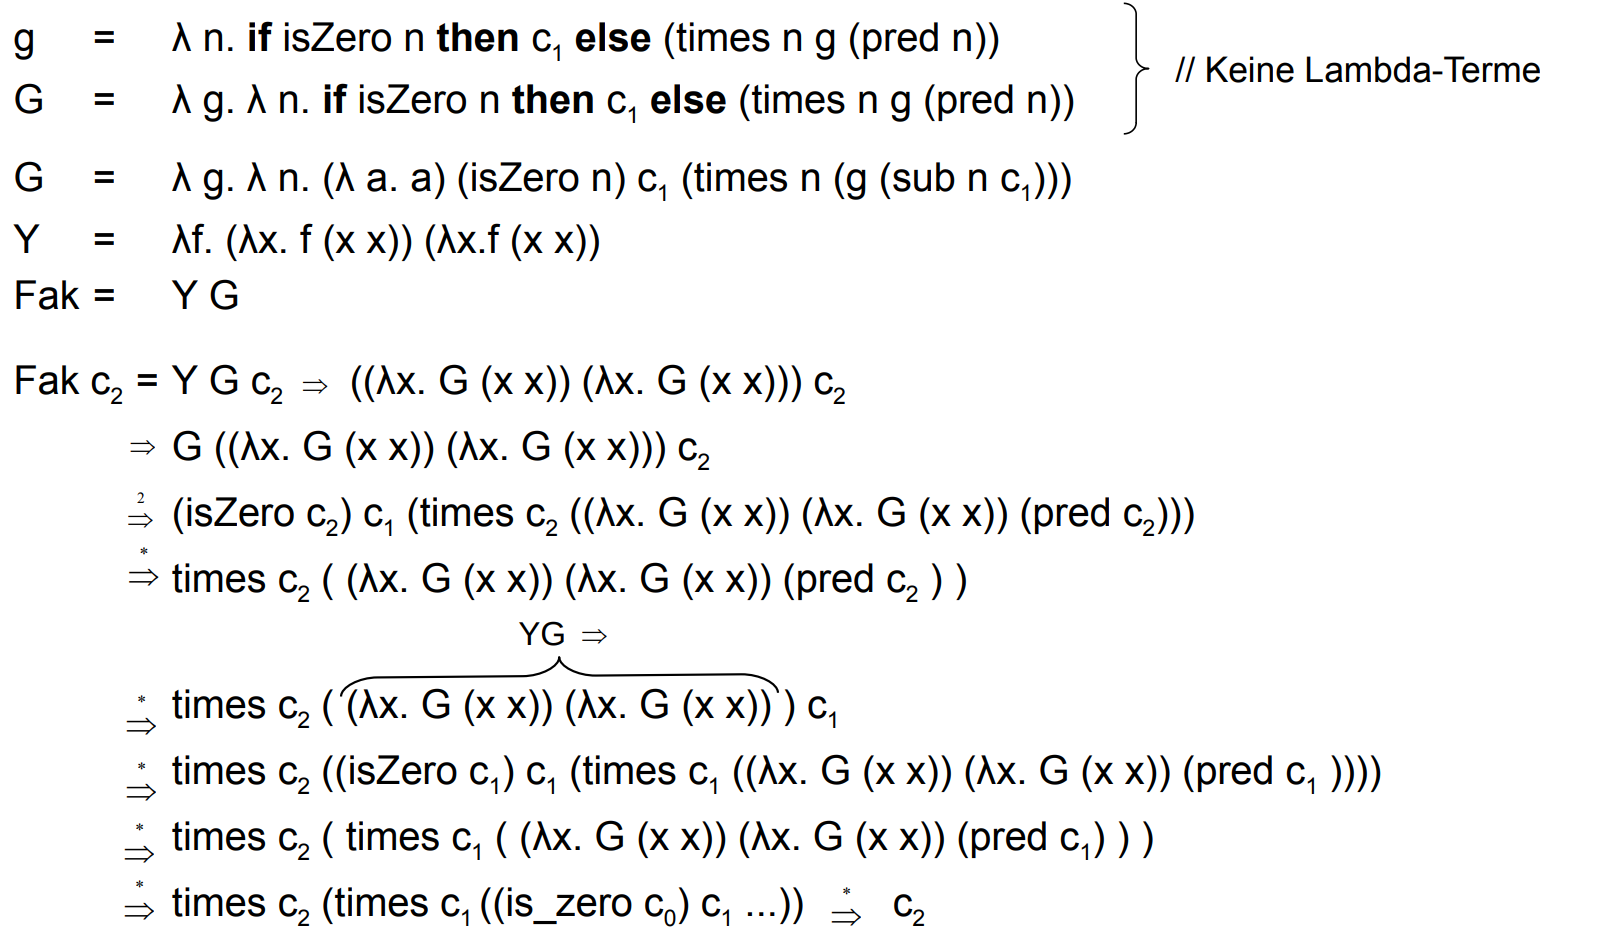
\includegraphics[width=0.4\linewidth]{Assets/Programmierparadigmen-Lambda_Abstraktion}
\end{center}

\subsubsection{Freie und gebundene Variablen}
\begin{itemize*}
  \item Die Menge der \color{blue} freien Variablen \color{black} eines Terms M wird mit FV(M) bezeichnet und ist wie folgt induktiv definiert:
  \begin{itemize*}
    \item $FV(x) = \{x\}$
    \item $FV(MN) = FV(M) \cup FV(N)$
    \item $FV(\lambda x.M) = FV(M) - \{x\}$
  \end{itemize*}
  \item Übung: Definieren sie analog die Menge der gebundenen Variablen GV(M)
  \item Ein Lambda-Term ohne freie Variablen heißt \color{blue}Kombinator \color{black}
  \item Einige besonders wichtige Kombinatoren haben eigene Namen:
  \begin{itemize*}
    \item Identitätsfunktion:\enspace\enspace \enspace \enspace\enspace\enspace\enspace I $\equiv$ $\lambda$x.x
    \item Konstanten-Funktional: \enspace $K \equiv\lambda xy.x$
    \item Fixpunkt-Kombinator: \enspace $Y\equiv\lambda f.(\lambda x.f(x x)) (\lambda x.f(x x))$
  \end{itemize*}
\end{itemize*}

\subsubsection{Ausführung von Lambda-Termen}
\colorbox{lightgray}{ \begin{minipage}[h]{.9\linewidth}
    \begin{tabular}{ l | l }
      Redex             & Ein $\lambda$-Term der Form ($\lambda x.t_1)t_2$ heißt Redex.                                                     \\
      $\beta$-Reduktion & entspricht der Ausführung der Funktionanwendung auf einem Redex:                                                  \\
                        & ($\lambda x.t_1)t_2 \Rightarrow t_1[x \rightarrow t_2]$                                                           \\
      Substitution      & $t_1[x \rightarrow t_2]$ erhält man aus dem Term $t_1$, wenn man alle freien Vorkommen von x durch $t_2$ ersetzt. \\
      Normalform        & Ein Term, der nicht weiter reduziert werden kann, heißt in Normalform
    \end{tabular}
  \end{minipage}
}

Beispiele:   
\begin{center}
  $$(\lambda x.x)y \Rightarrow x[x \rightarrow y] = y$$
  $$(\lambda x.x(\lambda x.x))(yz) \Rightarrow (x(\lambda x.x))[x \rightarrow (yz)] = ((yz)(\lambda x.x)$$
\end{center}

\subsubsection{Braucht man primitive Operationen?}
Nicht unbedingt - Kodierung mit Funktionen höherer Ordnung \\
Beispiel: let \\
\hspace*{14.5mm}let x = $t_1$ in $t_2$ wird zu ($\lambda x. t_2 )t_1$
\\
Beispiel: let x = g y in f x berechnet f(g y)\\
\hspace*{14.5mm} ($\lambda x.fx)(g y) \Rightarrow f(g y)$

  \subsection{Äquivalenz}
  \paragraph{$\alpha$-Äquivalenz}
  
  Namen gebundener Variablen
  \begin{itemize*}
    \item dienen letztlich nur der Dokumentation
    \item entscheidend sind die Bindungen
  \end{itemize*}
  
  \colorbox{lightgray}{
    \begin{minipage}[h]{.9\linewidth}
      $\alpha$-Äquivalenz \\
      $t_1$ und $t_2$ heißen $\alpha$-Äquivalent ($t_1 \stackrel{\alpha}{=} t_2$), wenn $t_1$ in $t_2$ durch konsistente Umbenennung der $\lambda$-gebundenen Variablen überführt werden kann. 
    \end{minipage}
  }
  
  Beispiele: 
  \begin{center}
    $$\lambda x.x \stackrel{\alpha}{=} \lambda y.y$$
    $$\lambda x.\lambda z.f(\lambda y.zy)x \stackrel{\alpha}{=} \lambda y.\lambda x.f(\lambda z.xz)y$$
  \end{center}
  aber
  \begin{center} 
    $$\lambda x.\lambda z.f(\lambda y.zy)x \stackrel{\alpha}{\neq} \lambda x.\lambda z.g(\lambda y.zy)x$$
    $$\lambda z.\lambda z.f(\lambda y.zy)z\stackrel{\alpha}{\neq} \lambda x.\lambda z.f(\lambda y.zy)x$$
  \end{center}
  
  \paragraph{$\eta$-Äquivalenz}

  Extensionalitäts-Prinzip: 
  \begin{itemize*}
    \item Zwei Funktionen sind gleich, falls Ergebnis gleich für alle Argumente
  \end{itemize*}
  \colorbox{lightgray} {
    \begin{minipage}[h]{.9\linewidth}
      $\eta$-Äquivalenz \\
      Terme $\lambda x.fx$ und f heißen $\eta$-äquivalent ($\lambda x.fx \stackrel{\eta}{=}  f$), falls x nicht freie Variable von f ist.
    \end{minipage}
  }
  
  Beispiele:
  $$\lambda x.\lambda y.f z x y \stackrel{\eta}{=}\lambda x.f z x$$
  $$f z \stackrel{\eta}{=}\lambda x.f z x$$
  $$\lambda x.x \stackrel{\eta}{=}\lambda x.(\lambda x.x)x$$
  aber $$\lambda x.f x x \stackrel{\eta}{\neq} f x$$
  
  \subsection{Kodierung boolscher Werte}
  Church Booleans
  \begin{itemize*}
    \item True wird zu: $C_{true} = \lambda t.\lambda f.t$
    \item False wird zu: $C_{false} = \lambda t.\lambda f.f$
    \item If-then-else wird zu: $If = \lambda a.a$
  \end{itemize*}
  
  Beispiel
  \begin{lstlisting}
    if True then x else y
\end{lstlisting}
  ergibt: $(\lambda a.a)(\lambda t- \lambda f.t) x y = (\lambda t.\lambda f.t) xy = (\lambda f.x)y \Rightarrow x$

  \begin{center}
    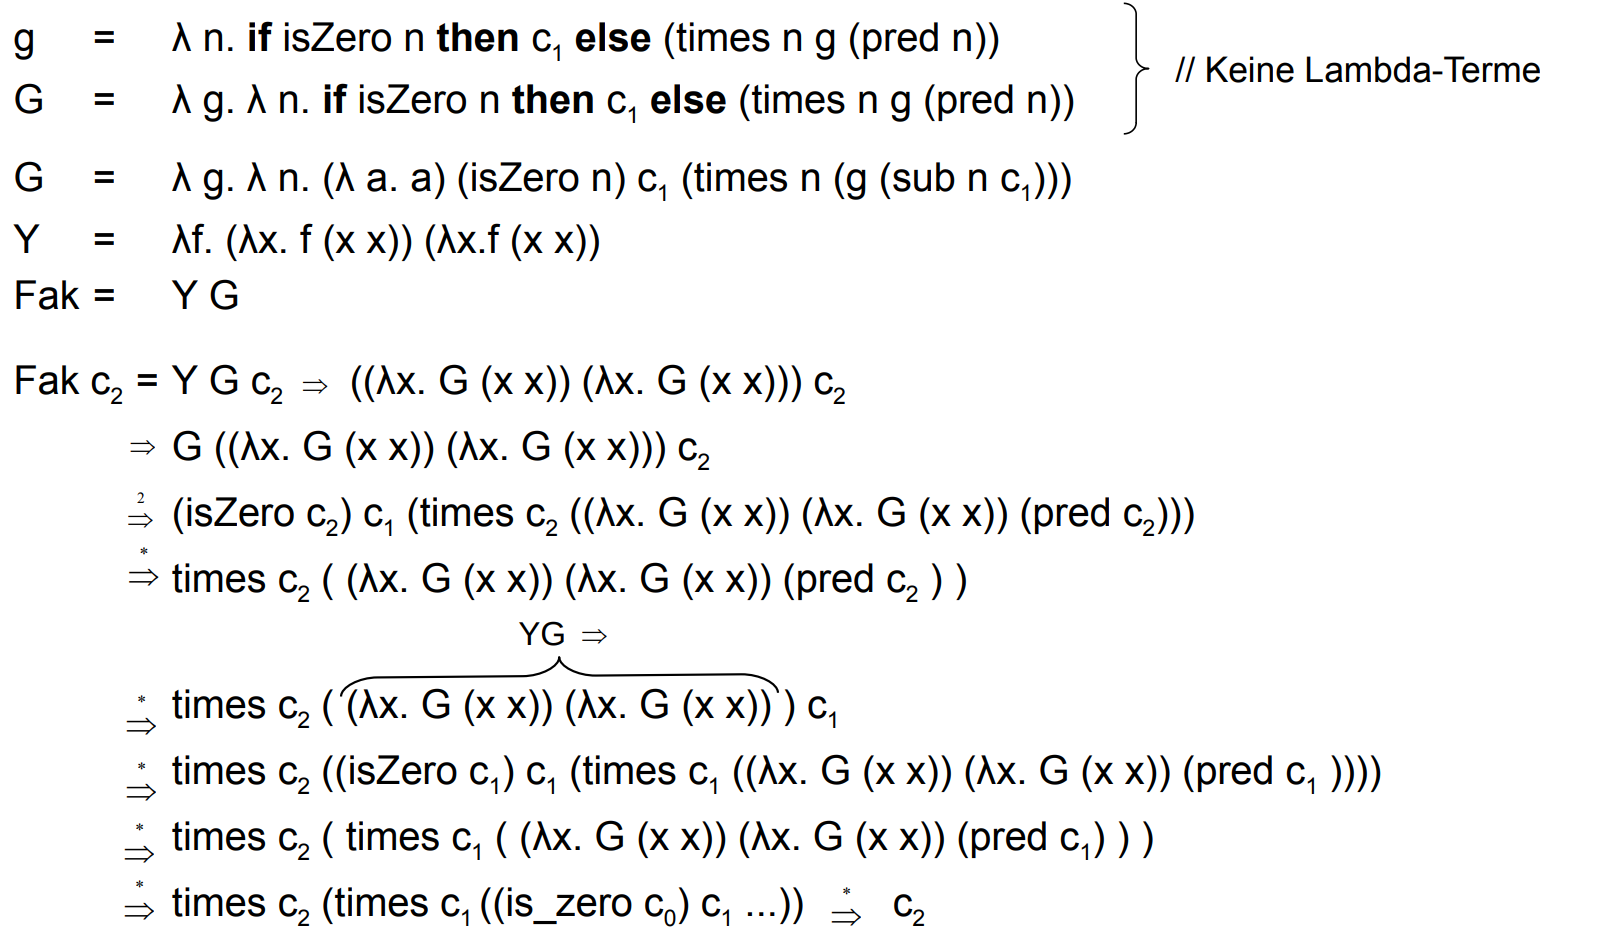
\includegraphics[width=0.4\linewidth]{Assets/Programmierparadigmen-Lambda_Abstraktion.png}
  \end{center}
  
  \begin{itemize*}
    \item if True then x else y ergibt:
    \subitem ($\lambda$\color{blue}a.a\color{black})(\color{red} $\lambda$t.$\lambda$f.t\color{black}) x y $\Rightarrow$ ($\lambda$\color{blue}t\color{black}.$\lambda$f.\color{blue}t\color{black}) \color{red}x\color{black} y $\Rightarrow$ ($\lambda$\color{blue}f\color{black}.x)\color{red}y\color{black} $\Rightarrow$ x
    \item $b_1$ \&\& $b_2$ ist äquivalent zu if $b_1$ then $b_2$ else False
    \subitem $\Rightarrow$  $b_1$ \&\& $b_2$ wird zu ($\lambda$a.a) $b_1$ $b_2$ $C_false$
    \subitem $\Rightarrow$  $b_1$ \&\& $b_2$ wird zu ($\lambda$a.a) $b_1$ $b_2$ ($\lambda$t.$\lambda$f.f)
    \item True \&\& True ergibt:
    \subitem \color{white} $\Rightarrow$ \color{black}($\lambda$\color{blue}a.a\color{black})\color{red}$C_true$ \color{black} $C_true$ ($\lambda$t.$\lambda$f.f)
    \subitem  $\Rightarrow$ ($\lambda$\color{blue}t\color{black}.$\lambda$f.\color{blue}t\color{black})\color{red}($\lambda$t.$\lambda$f.t)\color{black}($\lambda$t.$\lambda$f.f)
    \subitem $\Rightarrow$ ($\lambda$\color{blue}f\color{black}.($\lambda$t.$\lambda$f.t)) \color{red}($\lambda$t.$\lambda$f.f)\color{black} $\Rightarrow$ $\lambda$t.$\lambda$f.f = $C_true$
    \item $b_1 \lor b_2$ entspricht:
    \subitem if $b_1$ then True else $b_2$
    \item $\neg b_1$ entspricht:
    \subitem if $b_1$ then False else True
    \item $b_1 \Rightarrow b_2$ entspricht:
    \subitem if $b_1$ then $b_2$ else True
  \end{itemize*}
  
  \subsection{Kodierung natürlicher Zahlen}
  Eine natürliche Zahl drückt aus, wie oft etwas geschehen soll.
$c_0 = \lambda s.\lambda z.z$; $c_1=\lambda s.\lambda z.sz$; $c_2=\lambda s.\lambda z.s(sz)$;...;$c_n=\lambda s.\lambda z.s^n z$

  Arithmetische Operationen
  \begin{itemize}
    \item Addition:   $plus = \lambda m. \lambda n. \lambda s. \lambda z. m s (n s z)$
    \item Multiplikation: $times = \lambda m. \lambda n. \lambda s. n (m s) = \lambda m. \lambda n. \lambda s. \lambda z. n (m s) z$
    \item Exponentiation: $exp = \lambda m. \lambda n. n m = \lambda m. \lambda n. \lambda s. \lambda z. n m s z$
    \item Vorgänger:  $pred = \lambda n.\lambda s.\lambda x. n (\lambda y.\lambda z. z (y s))(K x)$
    \item Subtraktion: $sub = \lambda n.\lambda m. m pred n$
    \item Nullvergleich: $isZero = \lambda n. n (\lambda x. C false ) C true$
  \end{itemize}
  \begin{center}
    \includegraphics[width=0.4\linewidth]{Assets/Programmierparadigmen-kodierung-natürlicher-zahlen}
  \end{center}
  
  succ($c_2$) = ($\lambda$\color{blue}n\color{black}.$\lambda s.\lambda z.s$ (\color{blue}n\color{black} s z)) \color{red} ($\lambda$s.$\lambda z.s (s z))$ \color{black}
  \subitem $\Rightarrow\lambda s.\lambda z.s ((\lambda$\color{blue}s\color{black}.$\lambda z.$ \color{blue} s \color{black}(\color{blue}s\color{black} z)) s z)
  \subitem $\Rightarrow\lambda s.\lambda z.s((\lambda$\color{blue}z\color{black}.s (s \color{blue}z\color{black}))\color{red}z\color{black})
  \subitem $\Rightarrow\lambda s.\lambda z.s(s(s z)) = c_3$

  \subsection{Rechnen mit Church - Zahlen }
  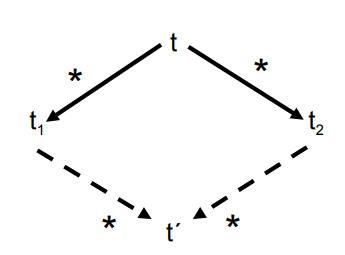
\includegraphics[width=0.4\linewidth]{Assets/Programmierparadigmen-diamant-eigenschaft}
  \begin{lstlisting}[language=erlang]
Runnable task = () -> {
  String me = Thread.currentThread().getName();
  System.out.println("Hallo " + me);
}

task.run();

Thread thread = new Thread(task);
thread.start();
\end{lstlisting}
  
  Idee zu exp: \\
  \subitem exp $c_m c_n \Rightarrow c_n c_m \Rightarrow (\lambda.\color{blue}s\color{black}.\lambda z.s^n z)\color{red}(\lambda s. \lambda z.s^m z)$ \color{black}
  \subsubitem $\Rightarrow \lambda z.(\lambda s. \lambda z.s^m z)^n z$
  \subitem (per Induktion über n) $\stackrel{\alpha \beta \eta}{\Rightarrow}\lambda s.\lambda z. \lambda z.{s^m}^n z = {c_m}^n$

  \begin{center}
    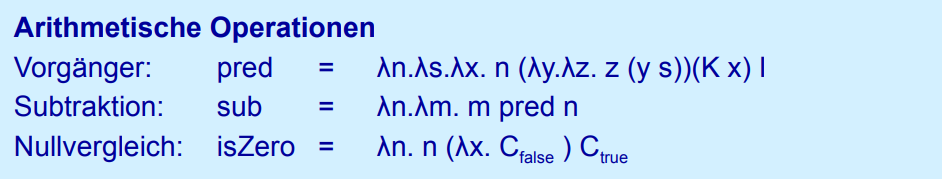
\includegraphics[width=0.4\linewidth]{Assets/Programmierparadigmen-Arithmetische-Operationen}
  \end{center}
  
  \subitem $isZero(c_0) = (\lambda\color{blue}n\color{black}.\color{blue}n\color{black}(\lambda x.C_{false})C_{true})\color{red} (\lambda s.\lambda z.z)\color{black}$
  \subsubitem $\Rightarrow (\lambda s. \lambda z. z)\color{red} (\lambda x.C_{false})\color{black} C_{true}$
  \subsubitem $\Rightarrow (\lambda \color{blue} z.z \color{black}) \color{red} C_{true} \Rightarrow C_{true}$
  (Bemerkung: I und K sind die Identitätsfunktion bzw. das Konstanten-Funktional)
  
  \begin{center}
    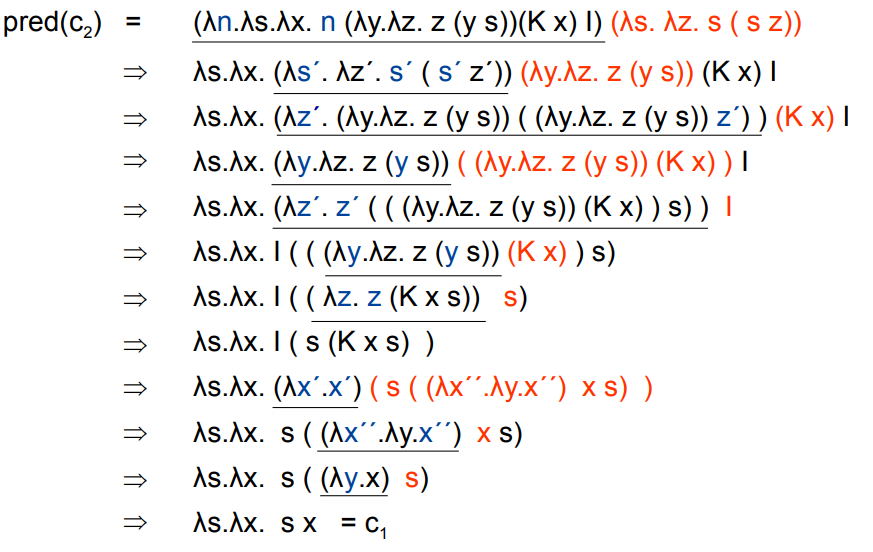
\includegraphics[width=0.4\linewidth]{Assets/Programmierparadigmen-Arithmetische-Operationen-2}
  \end{center}
  
  \subsection{Auswertungsstrategien}
  Wenn es in einem Term mehrere Redexe gibt, welchen reduziert man dann?
  $$(\lambda x.x)((\lambda x.x)(\lambda z.(\lambda x.x)z))$$
  $$(\lambda \color{blue}x.x\color{black})\color{red}((\lambda x.x)(\lambda z.(\lambda x.x)z)) \color{black}$$
  $$(\lambda x.x)((\lambda \color{blue}x.x\color{black})\color{red}(\lambda z.(\lambda x.x)z)\color{black})$$
  $$(\lambda x.x)((\lambda x.x)(\lambda z.(\lambda \color{blue}x.x\color{black})\color{red}z\color{black})$$
  $$(\lambda x.x)((\lambda x.x)(\lambda z.(\lambda x.x)z))$$
  
  Volle $\beta$-Reduktion: Jeder Redex kann jederzeit reduziert werden
  $$(\lambda x.x)((\lambda x.x)(\lambda z.(\lambda \color{blue}x.x\color{black})\color{red}z\color{black}))$$
  $$\Rightarrow(\lambda x.x)((\lambda\color{blue}x.x\color{black})\color{red}(\lambda z.z)\color{black})$$
  $$\Rightarrow(\lambda \color{blue}x.x\color{black})\color{red}(\lambda z.z)\color{black})$$
  $$\Rightarrow(\lambda z.z)\color{black} \nRightarrow$$
  $$(\lambda x.x)((\lambda x.x)(\lambda z.(\lambda x.x)z))$$
  
  Volle $\beta$-Reduktion: Jeder Redex kann jederzeit reduziert werden \\
  Normalreihenfolge: Immer der linkeste äußerste Redex wird reduziert
  $$(\lambda x.x)((\lambda\color{blue}x.x\color{black})\color{red}(\lambda z.(\lambda x.x)z))\color{black}$$
  $$\Rightarrow(\lambda \color{blue}x.x\color{black})\color{red}(\lambda z.(\lambda x.x)z)\color{black}$$
  $$\Rightarrow\lambda z.(\lambda\color{blue}x.x\color{black})\color{red}z\color{black}$$
  $$\Rightarrow(\lambda z.z)\color{black}) \nRightarrow$$
  
  \subsection{Fixpunktsatz und Rekursion}
  \subsubsection{Divergenz}
  Bisherige Beispiele werten zu einer Normalform aus. Aber:
  $$\omega = (\lambda \color{blue}x.x x\color{black})\color{red}(\lambda x.x x) \color{black} \rightarrow (\lambda x.x x)(\lambda x.x x)$$
  
$\lambda x.xx$ wendet sein Argument auf das Argument selbst an $\Rightarrow$ dadurch reproduziert $\omega$ sich selbst.
  
  \colorbox{lightgray}{
    \begin{minipage}[h]{.9\linewidth}
      Divergenz: \\
      Terme, die nicht zu einer Normalform auswerten, divergieren. 
      Diese modellieren unendliche Ausführungen.
    \end{minipage}
  }
  
  \subsubsection{Der Fixpunktsatz}
  \colorbox{lightgray}{
    \begin{minipage}[h]{.9\linewidth}
      Fixpunktsatz \\
      Für alle $F\in\Lambda$ existiert ein $X\in\lambda$ sodass gilt: $F X = X$
    \end{minipage}
  }
  
  \begin{itemize*}
    \item Der Fixpunktsatz besagt, dass im Lambda-Kalkül jeder Term einen Fixpunkt hat, d.h. einen Wert, der auf sich selber abgebildet wird.
    \item Beweis:
    \begin{itemize*}
      \item Zu jedem beliebigen F sei $W =\lambda x.F(x x)$ und $X = (W W)$
      \item Dann gilt: $X\equiv WW \equiv(\lambda x.F(x x)) W \equiv F(W W) \equiv F X$
    \end{itemize*}
    \item Bemerkungen:
    \begin{itemize*}
      \item Für einige Lambda-Terme ist die Identifikation eines Fixpunktes einfach, z.B. für den Term $\lambda x.x$ (alle Terme sind Fixpunkte)
      \item Für andere Terme, wie $\lambda xy.xy (= \lambda x.\lambda y.xy)$ ist das nicht so klar
      \item Der Beweis des Fixpunktsatzes ist konstruiv, d.h. er liefert zu jedem Lambda-Term einen Fixpunkt
    \end{itemize*}
  \end{itemize*}
  
  \subsubsection{Anwendung des Fixpunktsatzes}
  \begin{itemize*}
    \item Aufgabe: Berechne den Fixpunkt zum Term $\lambda xy.xy$
    \begin{itemize*}
      \item Lösungsansatz: $W\equiv\lambda x.(\lambda\color{blue}x\color{black}y.\color{blue}x\color{black}y)\color{red}(xx) \color{black} \equiv\lambda x.\lambda y.(x x)y \equiv \lambda xy.(xx)y$
      \item Damit ist der gesuchte Fixpunkt $X\equiv((\lambda xy.(xx)y)(\lambda xy.(xx)y))$
      \item Nachrechnen:
      \begin{description*}
        \item[ \space ] $(\lambda xy.xy) ((\lambda xy.(xx)y) (\lambda xy.(xx)y))$
        \item[$\equiv$] $(\lambda \color{blue}x\color{black}.\lambda y. \color{blue} x \color{black} y) \color{red} ((\lambda xy.(xx)y) (\lambda xy.(xx)y)$ \color{black}
        \item[$\equiv$] $\lambda \color{blue}y \color{black}.((\lambda xy.(xx)y)) (\lambda xy.(xx)y) \color{red}y\color{black}$
        \item[$\equiv$] $(\lambda xy.(xx)y)(\lambda xy.(xx)y)$
        \item[$\equiv$] X
      \end{description*}
    \end{itemize*}
    \item Bemerkung: Der so für die Identitätsfunktion $\lambda x.x$ konstruierte Fixpunkt ist übrigens $(\lambda x.xx)(\lambda x.xx)$, er spielt die besondere Rolle des Standardterms $\bot$ für nicht-terminierende Ausführungen
  \end{itemize*}
  
  \subsubsection{Der Fixpunkt-Kombinator}
  \colorbox{lightgray}{
    \begin{minipage}[h]{.9\linewidth}
      Im Ergebnis unserer Diskussion des Fixpunktsatzes definieren wir den Fixpunkt-Kombinator wie folgt: $$Y \equiv \lambda f.(\lambda x.f(xx)) (\lambda x.f(xx))$$
    \end{minipage}
  }
  \begin{itemize*}
    \item Dieser Kombinator spielt eine wichtige Rolle bei der Definition rekursiver Funktionen im Lambda-Kalkül, wie wir im folgenden sehen werden
    \item Für jeden Lambda-Term M gilt: $Y M = M (Y M)$
    \begin{itemize*}
      \item Beweisidee: zeige, dass beide Terme auf einen identischen Term reduziert werden können
    \end{itemize*}
    \item Der Term Y ist übrigens nicht der einzige Kombinator, der Fixpunkte zu Lambda-Termen konstruiert
    \begin{itemize*}
      \item A. Turing: $\Theta \equiv (\lambda xy.y(xxy)) (\lambda xy.y(xxy))$
    \end{itemize*}
  \end{itemize*}
  
  \subsubsection{Rekursion im Lambda-Kalkül}
  \begin{itemize*}
    \item Die bisher definierten Funktionen waren alle nicht-rekursiv
    \item Viele Funktionen kann man aber nur unter Zuhilfenahme von Rekursion (bzw. Iteration) beschreiben
    \item In üblichen Programmiersprachen werden rekursive Funktionsdefinitionen durch die Verwendung von Namen für Funktionen möglich - man verwendet hierbei einfach den Namen der gerade zu definierenden Funktion im Rumpf der Definition:
    \begin{lstlisting}
    \item fun fak(i) -> if (i = 0) then 1 else i * fak(i-1).
  \end{lstlisting}
    \item Im Lambda-Kalkül gibt es jedoch keine Namen für Funktionen:
    \begin{itemize*}
      \item Daher stellt man eine rekursive Funktion f mittels einer Funktion G dar, die einen zusätzlichen Parameter g hat, an den man dann G selber bildet
      \item Schaut kompliziert aus, ist es auch (Q-Q)
      \item Warum so kompliziert? Damit die Definition von G im eigenen Rumpf verfügbar ist
    \end{itemize*}
  \end{itemize*}
  
  \subsubsection{Rekursive Funktionen sind Fixpunkte}
  \begin{itemize*}
    \item Rekursive Funktion von g
    \begin{itemize*}
      \item $g = \lambda n...g...n...$ Rumpf verwendet g
    \end{itemize*}
    \item Daraus gewinnt man das Funktional
    \begin{itemize*}
      \item $G = \lambda g.\lambda n...g...n...$
    \end{itemize*}
    \item Falls G einen Fixpunkt g* hat, d.h. $G(g*) = g*$, so
    \begin{itemize*}
      \item $g* = G(g*) = \lambda n...g*...n$
    \end{itemize*}
    \item Vergleiche: $g = \lambda n...g...n...$
  \end{itemize*}
  \begin{center}
    Rekursive Definition $\Leftrightarrow$ Fixpunkt des Funktionals
  \end{center}
  \begin{itemize*}
    \item Beispiel: Fakultät
    \begin{itemize*}
      \item $g = \lambda n. $ if isZero n then $c_1$ else (times n g(pred n)) - rekursiv
      \item $G = \lambda g.\lambda n.$ if isZero n then $c_1$ else (times n g(pred n)) - funktional
    \end{itemize*}
  \end{itemize*}
  
  \subsubsection{Der Fixpunktkombinator dient als Rekursionsoperator}
  Wir berechnen den gesuchten Fixpunkt des Funktionals G mit dem Fixpunktkombinator, der somit als Rekusrsionsoperator dient: 
  
  \color{blue} Rekursionsoperator \color{black}
  $$Y = \lambda f.(\lambda x.f(xx))(\lambda x.f(xx))$$
  $$Y f = (\lambda \color{blue}f\color{black}.(\lambda x.\color{blue}f\color{black}(xx))(\lambda x.\color{blue}f\color{black}(xx))) \color{red}f\color{black}$$
  $$\Rightarrow (\lambda \color{blue}x\color{black}.f(\color{blue}xx\color{black})) \color{red}(\lambda x.f(xx))\color{black}$$
  $$\Rightarrow f((\lambda x.f(xx)) (\lambda x.f(xx)) \Leftarrow f(Yf) ())$$
  \color{black}
  \subitem also \space\space\space \space $f(Yf) \stackrel{\beta}{=} Yf$ \\
  d.h. \space\space\space Yf ist Fixpunkt von f
  
  \paragraph{Beispiel: Fakultät im Lambda-Kalkül}
  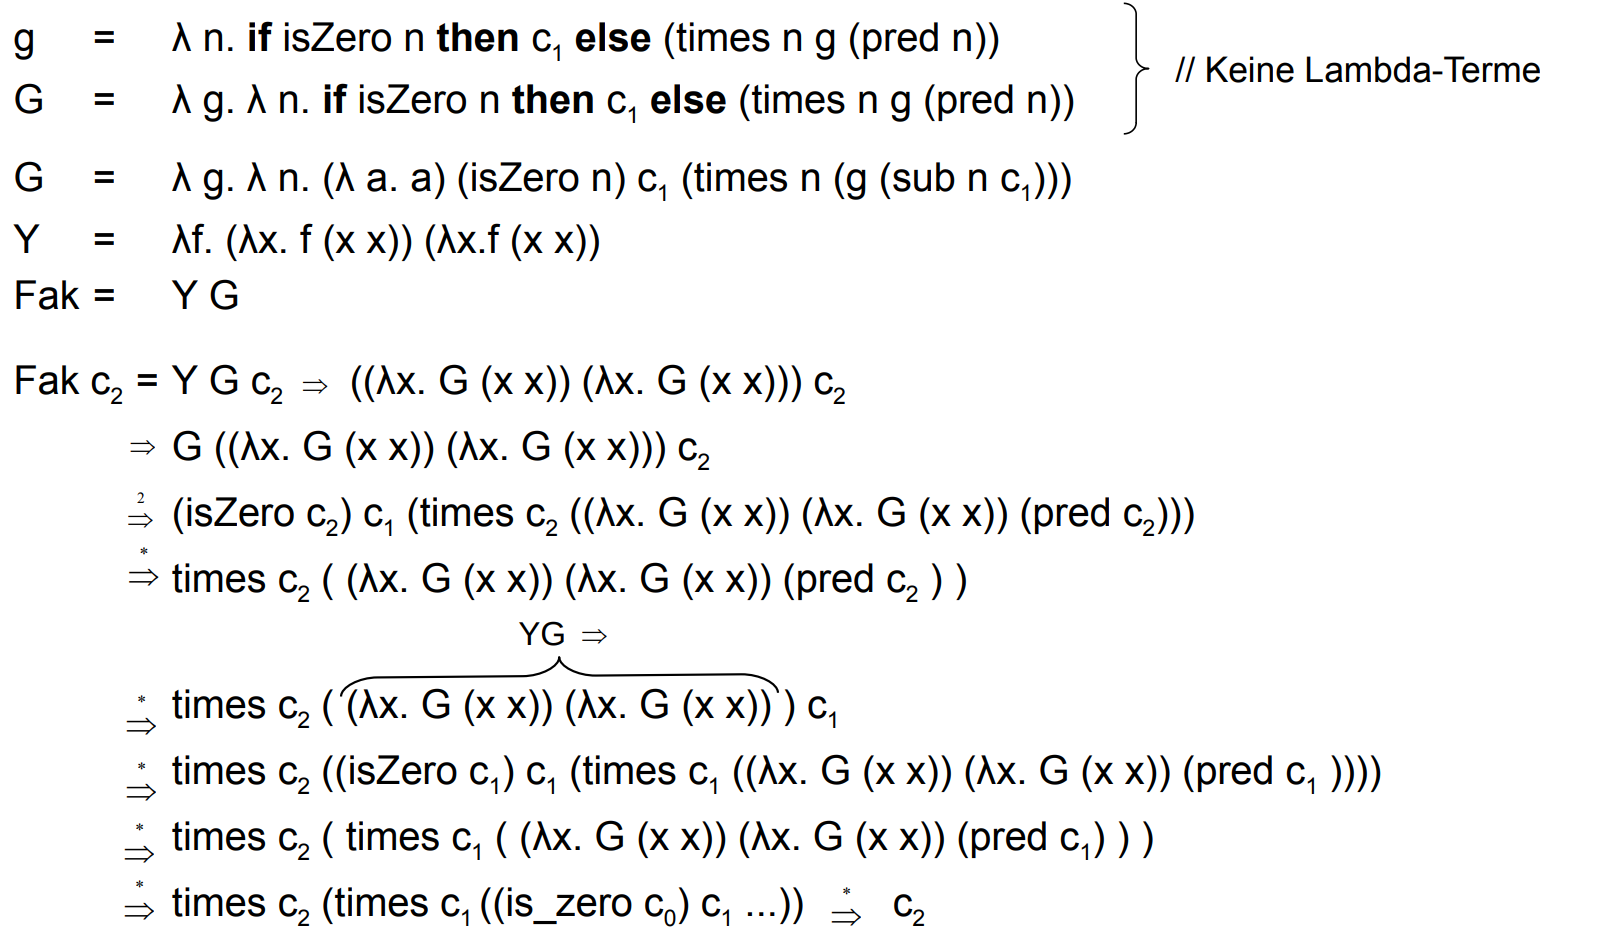
\includegraphics[width=.4\linewidth]{Assets/Programmierparadigmen-Lambda_Abstraktion}
  
  \subsection{Ausdrucksstärke des Lambdakalküls}
  \begin{itemize*}
    \item Im Folgenden wollen wir zeigen, dass der Lambda-Kalkül genau die rekursiven Funktionen beschreibt
    \item Eine numerische Funktion ist eine Abbildung $f:\mathbb{N}^k \rightarrow \mathbb{N}$ mit $k\in\mathbb{N} \cap \{0\}$
    \item Wir definieren hierzu:
    \begin{itemize*}
      \item Anfangsfunktionen:
      \begin{itemize*}
        \item Projektion: $U_i^k (n_1,n_2,...,n_k) = n_i$ für $1<=i<=k$
        \item Nullfunktion: $Z(n) = 0$
        \item Nachfolger: $S(n) = n+1$
      \end{itemize*}
      \item Minimalisierung:
      \begin{itemize*}
        \item Für eine Relation $P(m)$ bezeichne $\mu m[P(m)]$ die kleinste Zahl m sodass P(m) gilt.
      \end{itemize*}
    \end{itemize*}
    \item Bemerkung: im Folgenden notieren wir $n_1,n_2,...,n_k$ kurz als $\overline{n_k}$
    \item Eine numerische Funktion ist Lambda-definierbar, wenn es einen Kombinator M gibt, sodass $M\overline{n_k} = f(\overline{n_k})$
  \end{itemize*}
  
  \begin{itemize*}
    \item Im folgenden sei C eine Klasse von numerischen Funktionen, und es gelte $g,h,h_1,h_2,...,h_m \in C$
    \item Wir definieren nun die folgenden Eigenschaften:
    \begin{itemize*}
      \item C ist \color{blue} abgeschlossen unter Komposition\color{black}, wenn für jede Funktion f, die über $f(\overline{n_k}):= g(h_1(\overline{n_k}),...,h_m(\overline{n_k}))$ definiert ist, gilt $f \in C$
      \item C ist \color{blue} abgeschlossen unter primitiver Rekursion\color{black}, wenn für jede Funktion f, die über
      $$f(0,\overline{n_k}) = g(\overline{n_k})$$
      $$f(j+1, \overline{n_k}) = h(f(j,\overline{n_k}),j,\overline{n_k})$$
      definiert ist, gilt: $f \in C$
      \item C ist \color{blue} abgeschlossen unter unbeschränkter Minimalisierung \color{black}, wenn für jede Funktion f, die über $f(\overline{n_k})=\mu m[g(\overline{n_k},m)= 0]$ definiert ist (wobei für alle $\overline{n_k}$ ein m existiere, sodass $g(\overline{n_k},m) = 0$ ist), gilt $f \in C$
    \end{itemize*}
  \end{itemize*}
  
  \colorbox{lightgray}{\begin{minipage}[h]{.9\linewidth}
      Definition: \\
      Die Klasse der rekursiven Funktionen ist die kleinste Klasse numerischer Funktionen, die alle oben genannten Anfangsfunktionen enthält und abgeschlossen ist unter Komposition, primitiver Rekursion und unbeschränkter Minimalisierung
    \end{minipage}
  }
  
  \begin{itemize*}
    \item \color{blue} Lemma 1: Die Anfangsfunktionen sind Lambda-definierbar \color{black}
    \item Beweis:
    \begin{itemize*}
      \item $U_i^k = \lambda x_1 x_2 ... x_k.x_i$
      \item $S = \lambda n.\lambda s. \lambda z.s(nsz)$ (siehe succ bei Churchzahlen)
      \item $Z = \lambda fx.x$ (siehe $c_0$ bei Churchzahlen)
    \end{itemize*}
  \end{itemize*}
  
  \begin{itemize*}
    \item  \color{blue} Lemma 2: Die Lambda-definierbaren Funktionen sind abgeschlossen unter primitiver Rekursion \color{black}
    \item Beweis: Sei f definiert über
    \begin{center}
      $$f(0,\overline{n_k}) = g(\overline{n_k})$$
      $$f(j+1, \overline{n_k}) = h(f(j, \overline{n_k}),j,\overline{n_k})$$
    \end{center}
    und seien g und h Funktionen (die per Induktionsvoraussetzung) durch die Lambda-terme G und H berechnet werden
    \begin{itemize*}
      \item Intuitiv kann f berechnet werden, indem man überprüft ob j = 0 ist, und wenn ja $g(\overline{n_k})$, ansonsten $h(f(j, \overline{n_k}),j,\overline{n_k})$
      \item Ein Term M hierfür existiert laut Fixpunktsatz und es gilt:
      $M \equiv Y (\lambda f\:x\: \overline{y_k}.if(isZero \: x)(G\:\overline{y_k})(H(f(pred\: x)\overline{y_k})(pred \: x)\overline{y_k}))$
    \end{itemize*}
  \end{itemize*}
  
  \begin{itemize*}
    \item \color{blue} Lemma 3: Die Lambda-definierbaren Funktionen sind abgeschlossen unter unbeschränkter Minimalisierung \color{black}
    \item Beweis:
    \begin{itemize*}
      \item Sei f über $f(\overline{n_k}) = \mu m[g(\overline{n_k},m) = 0]$ definiert, wobei g (per Induktionsvoraussetzung) durch den Lambda-Term G berechnet wird
      \item Intuitiv kann man f berechnen, indem man bei 0 beginnend für m überprüft, ob $g(\overline{n_k},m) = 0$ ist, und wenn ja m ausgibt, ansonsten die Überprüfung mit $m+1$ fortsetzt
      \item Ein Term für eine solche Funktion kann laut Fixpunktsatz konstruiert werden und man erhält mit Anwendung des Fixpunktkombinators zunächst: $$N \equiv Y (\lambda f \: \overline{x_k} \: y. if(isZero \: (G \: \overline{x_k} \: y))y(f\:\overline{x_k}\:(succ \: y)))$$
      \item Nun definiert man die Funktion f durch den folgenden Term M: $$M \equiv \lambda \overline{x_k}.N \: \overline{x_k} \: c_0$$
    \end{itemize*}
  \end{itemize*}
  
  \begin{center}
    \includegraphics[width=.4\linewidth]{Assets/Programmierparadigmen-kodierung-natürlicher-zahlen}
  \end{center}
  \begin{itemize*}
    \item Aus den Lemmata 1 bis 3 folgt nun der Satz:\\
    \colorbox{lightgray}{
      \begin{minipage}[h]{.9\linewidth}
        Alle rekursiven Funktionen sind Lambda-definierbar
      \end{minipage}}
  \end{itemize*}
  
  
  \subsection{Berechnungsreihenfolgen und Konfluenz}
  \subsubsection{Noch einmal Auswertungsstrategien}
  \begin{itemize*}
    \item Bei unserer initialen Betrachtung der Auswertungsstrategien haben wir die volle $\beta$-Rekursion und die Normalreihenfolge kennengelernt
    \item Nun wollen wir unsere Betrachtungen hierzu noch einmal vertiefen und definieren zunächst:
    \begin{itemize*}
      \item Ein Redex wird als \color{blue} 'äußerst' (outermost) \color{black} bezeichnet, wenn er nicht Teil eines anderen Redex ist.
      \item Ein Redex wird als \color{blue} 'innerst' (innermost) \color{black} bezeichnet, wenn er keinen eigenständigen Redex beinhaltet
    \end{itemize*}
    \item Mit diesen Begriffen können im folgenden die gebräuchlichsten Auswertungsstrategien formuliert werden
    \begin{itemize*}
      \item \color{blue} Normal Order: \color{black} Evaluiere Argumente so oft, wie sie verwendet werden
      \item \color{blue} Applicative Order: \color{black} Evaluiere Argumente einmal
      \item \color{blue} Lazy Evaluation: \color{black} Evaluiere Argumente höchstens einmal
    \end{itemize*}
    \item Eine zentrale Kernfrage: \color{blue} Welche Auswertungsstrategie führt (möglichst schnell) zu einem nicht weiter reduzierbaren Term?
    \color{black}
    \begin{itemize*}
      \item Bei unserer beispielhaften Berechnung des Terms Fak $c_2$ haben wir nach der initialen Anwendung des Fixpunktkombinators zunächst den Term isZero $c_2$ reduziert.
      \item Ebenso hätten wird den weiter innen stehenden Fixpunktkombinator zuerst erneut anwenden können(bei voller $\beta$-Reduktion kann jeder Term jederzeit reduziert werden).
      \item Auf diese Weise hätten wir unendlich oft vorgehen, damit einen immer länger werdenden Term ableiten können und somit nicht das gewünschte Resultat $c_2$ berechnet.
    \end{itemize*}
    \item Eine weitere Kernfrage: Angenommen mehrere unterschiedliche Reduktionsreihenfolgen führen zu einem nicht weiter zu reduzierenden Ergebnis - \color{blue} führen all diese Reihenfolgen zum gleichen Ergebnis? \color{black}
    \item Wir definieren zuerst einen zentralen begriff in diesem Zusammenhang:
    \colorbox{lightgray}{\begin{minipage}[h]{.9\linewidth}
        Ein Transitiosnsystem $(D,\rightarrow*)$ heißt genau dann konfluent, wenn für alle $t,t_1,t_2 \in D$ gilt: wenn  $ t \rightarrow* t_1$ und $t \rightarrow* t_2$, dann gibt es ein $t' \in D$ mit $t_1 \rightarrow* t'$ und $t_2 \rightarrow* t'$
      \end{minipage}}
    \item Wenn der Lambda-Kalkül konfluent ist, kann hieraus gefolgert werden, dass unterschiedliche Reduktionsreihenfolgen, die zu einer nicht mehr weiter zu reduzierenden Form führen, somit auf den gleichen Term führen müssen.
    \item Achtung: hieraus kann nicht gefolgert werden, dass alle Reduktionsreihenfolgen auf den gleichen Term führen, da dies ja nur für 'terminierende' Reduktionsreihenfolgen gilt!
  \end{itemize*}
  
  \subsubsection{Church-Rosser-Eigenschaft}
  \color{blue} Satz (Church-Rosser) \\
  Der untypisierte $\lambda$-Kalkül ist konfluent: Wenn $t \stackrel{*}{\Rightarrow} t_1$ und $t \stackrel{*}{\Rightarrow} t_2$, dann gibt es ein t' mit $t_1 \stackrel{*}{\Rightarrow} t'$ und $t_2 \stackrel{*}{\Rightarrow} t'$
  \color{black}
  
  \begin{center}
    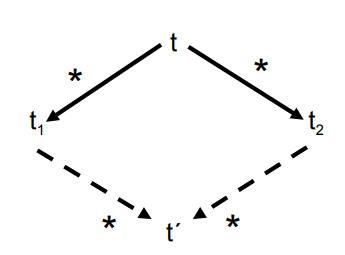
\includegraphics[width=0.25\linewidth]{Assets/Programmierparadigmen-diamant-eigenschaft.png}
    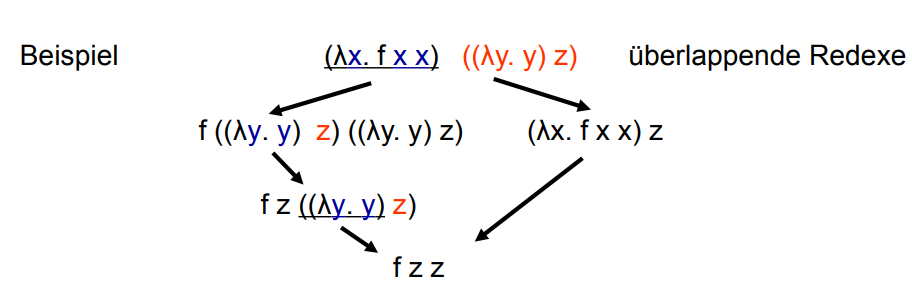
\includegraphics[width=0.25\linewidth]{Assets/Programmierparadigmen-diamant-beispiel}
  \end{center}
  
  Beweisidee: Definiere $\stackrel{\rightarrow}{\rightarrow}$ als 'parallele' $\beta$-Reduktion.
  \begin{itemize*}
    \item Es gilt: $\Rightarrow \subseteq \stackrel{\rightarrow}{\rightarrow} \subseteq \stackrel{*}{\Rightarrow}$
    \item Zeige Diamant Eigenschaft für $\stackrel{\rightarrow}{\rightarrow}$
  \end{itemize*}
  
  \subsubsection{Eindeutigkeit der Normalform}
  \color{blue} Korollar (Eindeutigkeit der Normalform) \newline
  Die Normalform eines $\lambda$-Terms ist - sofern sie existiert - eindeutig. \color{black}
  \newline
  \newline
  Beweis: 
  \begin{itemize*}
    \item $t_1$ und $t_2$ Normalformen von t, d.h. $t \stackrel{*}{\Rightarrow} t_1 \nRightarrow$ und $t \stackrel{*}{\Rightarrow} t_2 \nRightarrow$
    \item Nach Chruch-Rosser gibt es t' mit $t_1 \stackrel{*}{\Rightarrow} t'$ und $t_2 \stackrel{*}{\Rightarrow} t'$
    \item Nach Annahme $t_1 \nRightarrow$ und $t_2 \nRightarrow$, also $t_1 = t' = t_2$
  \end{itemize*}\ \newline
  \color{blue}
  Bei terminierenden $\beta$-Reduktionen ist irrelevant, welchen Redex man zuerst reduziert!\color{black}
  \subsection{Auswertung von Parametern in Programmiersprachen}
  \subsubsection{Behandlung von Parametern in Programmiersprachen}
  \begin{itemize*}
    \item Die Art und Weise, wie in einer Programmiersprache Parametter übergeben - d.h. wie die Reihenfolge und die Zeitpunkte ihrer Auswertung gehandhabt - werden, hat Einfluss auf wichtige Eigenschaften der Sprache:
    \begin{itemize*}
      \item Effizienz der Berechnungen
      \item Termininerungsverhalten
      \item Ausdruckskraft
    \end{itemize*}
    \item Hierbei ist es insbesondere von Interesse, wie Parameter gehandhabt werden, deren Werte undefiniert sind (z.B. 1/0)\newline
    \colorbox{lightgray}{
      \begin{minipage}[h]{.9\linewidth}
        Wir definieren zunächst den zentralen begriff 'strikt': \newline Eine n-stellige Funktion heißt strikt im k-ten Argument $(1<=k<=n)$, wenn gilt: $f(x_1,x_2,...,x_{k-1},\bot,x_{k+1},...,x_n)=\bot$
      \end{minipage}}
    \item Ein undefiniertes Argument führt hier zu einem undefinierten Resultat
    \item Grundsätzlich kann man die Auswertungsstrategien von Programmiersprachen in strikte und nicht-strikte Strategien einteilen; sehr gebräuchlich sind dabei insbesondere:
    \begin{itemize*}
      \item Call by Value: Ausdrücke, die Parameter bei einem Funktionsaufruf beschreiben, werden vor der Übergabe an die Funktion vollständig ausgewertet
      \item Call by Name: Ausdrücke, die Parameter bei einem Funktionsaufruf beschreiben, werden nicht bei Übergabe, sondern erst dann ausgewertet, wenn sie in der aufgerufenen Funktion tatsächlich benötigt werden
    \end{itemize*}
    \item Beide Varianten haben spezifische Vor- und Nachteile:
    \begin{itemize*}
      \item Call by Value: weniger Berechnungsaufwand, wenn ein Parameter mehr als einmal im Funktionsrumpf vorkommt; weniger Speicheraufwand bei der Übergabe
      \item Call by Name: weniger Berechnungsaufwand, wenn ein Argument nicht zum Ergebnis beiträgt; höherer Aufwand bei Übergabe
    \end{itemize*}
    \item Die Programmiersprache Erlang realisiert grundsätzlich eine strikte Handhabung von Parametern, da sie die Strategie Call by Value verwendet
    \item Allerdings wird bei der Definition einer Funktion der resultierende Wert erst dann berechnet, wenn die Funktion ausgewertet wird
    \begin{itemize*}
      \item Das erlaubt über den Umweg zusätzlicher Funktionsdefinitionen auch die Realisierung einer nicht-strikten Auswertungsstrategie - ermöglicht Nachbildung der sogenannten Lazy-Evaluation
      \item hierbei wird ein nicht-strikt zu evaluierendes Argument als Resultat einer anonymen nullstelligen Funktion (ohne Parameter) 'verpackt'
      \item Im Rumpf der eigentlichen Funktion wird diese Funktion dann ausgewertet (= aufgerufen), wenn feststeht, dass dieses Argument für die Berechnung des Ergebnisses benötigt wird
      \item Andere funktionale Sprachen wie Haskell oder Gofer verwenden Call by Name und realisieren damit grundsätzlich Lazy-Evaluation
    \end{itemize*}
    
    \begin{lstlisting}[language=erlang]
    -module(lazy).
    -export([test1/3, test2/3]).
    test1(P, A, B) -> % A and B are arbitrary values
      if
        P==true   -> A;
        P==false  -> B
     end.
    test2(P, A, B) -> % A and B have to be functions
      if
        P==true   -> A();
        P==false  -> B()
     end.
  \end{lstlisting}
    
    \begin{lstlisting}
  > lazy:test1(true, 3, 4/0).
  ** exception error: bad argument in an arithmetic expression in operator '/'/2 called as 4 / 0
  > lazy:test2(true, fun() -> 3 end, fun() -> 4/0 end).
  3
  \end{lstlisting}
    
    \item Erläuterungen:
    \begin{itemize*}
      \item Im zweiten Beispiel wird der Rückgabewert der übergebenen Funktionne nur ausgewertet, wenn sie im Rumpf der auszuführenden Funktion aufgerufen werden
      \item Innerhalb von Erlang-Modulen kann man sich mit Hilfe einer Macro-Definition Schreibarbeit sparen:
      \begin{lstlisting}[language=erlang] 
      -define(DELAY(E), fun() -> E end).
      check() -> test2(true, ?DELAY(3), ?DELAY(4/0)).
    \end{lstlisting}
    \end{itemize*}
    \item Je nachdem, ob und wie häufig ein übergebener Parameter im Funktionsrumpf benötigt wird, können bei Lazy-Evaluation Berechnungen
    \begin{itemize*}
      \item komplett eingespart oder
      \item (in identischer Form) wiederholt erforderlich werden
      \item Unter Umständen kann man in der betreffenden Funktion durch Einführung einer temporären Variable redundante Mehrfachberechnungen einsparen ($\rightarrow$ Call by Need)
    \end{itemize*}
    \item Die Parameterübergabe ist bei Call by Name in der Regel aufwändiger als bei Call by Value
    \begin{itemize*}
      \item Die meisten Programmiersprachen (Java, C, C++, Pascal etc.) verwenden daher Call by Value ($\rightarrow$ strikte Auswertung)
      \item Eine Ausnahme wird oft bei dem IF-Konstrukt gemacht (der auszuführende Code ist hier ja meist auch kein Parameter)
    \end{itemize*}
    \item Zu Ausdrucksstärke: während strikte Funktionen durch die Strategie Call by Value realisiert werden, ist es nicht so, dass Lazy Evaluation es erlaubt, alle nicht-strikten Funktionen zu realisieren
    \begin{itemize*}
      \item Die folgenden Gleichungen definieren eine nicht-strikte Multiplikation $\otimes$ auf der Basis der Multiplikation · für Zahlen:
      $$0 \otimes y = 0$$
      $$x \otimes 0 = 0$$
      $$x \otimes y = x * y$$
      \item Wenn ein Arguemnt undefiniert ist, dann liefert $\otimes$ ein Ergebnis, sofern das andere Argument zu 0 evaluiert wird ($\rightarrow fak(-1) \otimes (fak(3)-6)$)
      \item Implementiert werden kann die Funktion nur durch eine Art von paralleler Auswertung mit Abbruch der anderen Berechnung sobald 0 als Resultat berechnet und zurückgegeben wurde
    \end{itemize*}
    \item Wir betrachten nun die Beziehungen zwischen Parameterbehandlung in Programmiersprachen und Reduktion von Lambda-Termen
  \end{itemize*}
  
  \subsubsection{Auswertungsstrategien \& Programmiersprachen}
  \color{blue} Werte in Programmiersprachen wie Haskell: \color{black}
  \begin{itemize*}
    \item Primitive Werte: 2, True
    \item Funktionen: ($\backslash x \rightarrow x$), ($\&\&$), ($x\rightarrow(\backslash y\rightarrow y+y)x$)
  \end{itemize*}
  
  \color{blue} Werte im $\lambda$-Kalkül:
  \color{black} \begin{itemize*}
    \item Abstraktionen: $c_2 = \lambda s. \lambda z.s\;(s\;z),\;\;\; C_{true} = \lambda t- \lambda f.t,\;\;\; \lambda x.x,\;\;\; \newline \lambda b_1. \lambda b_2.\;b_1\; b_2 (\lambda t.\lambda f.\;f),\;\;\; \lambda x.\;(\lambda y.\;plus\; yy)x$
  \end{itemize*}
  \color{blue} Auswertungsstrategie: \color{black} Keine weitere Reduzierung von Werten \newline
  Reduziere keine Redexe unter Abstraktionen (umgeben von $\lambda$):\newline
$\Rightarrow$ call-by-name, call-by-value
  \subsubsection{Call-By-Name}
  Call-By-Name: Reduziere linkesten äußersten Redex
  \begin{itemize*}
    \item Aber nicht falls von einem $\lambda$ umgeben \newline
    \subitem $(\lambda y. (\lambda x.y(\lambda z.z)x))\color{red} ((\lambda x.x)(\lambda y.y))$ \color{black} \newline
    \subitem	$(\lambda x.((\lambda \color{blue}x.x\color{black}) \color{red}(\lambda y.y)\color{black})(\lambda z.z)x)$
    \begin{center}
      \item Intuition: Reduziere Argumente erst, wenn benötigt
    \end{center}
  \end{itemize*}
  
  Auswertung in Haskell: \color{blue} Lazy-Evaluation = call-by-name (+sharing)\color{black}
  \begin{itemize*}
    \item Standard-Auswertungsstrategie für Funktionen/Konstruktoren
    \item listOf x = x : listOf x
    \item 3: listOf 3 $\nRightarrow$
    \item (div 1 0) : (6 : [])
    \item tail ((div 1 0): (6 : [])) $\Rightarrow$ 6 : [] $\nRightarrow$
  \end{itemize*}
  
  \subsubsection{Call-By-Value}
  Call-By-Value: Reduziere linkesten Redex
  \begin{itemize*}
    \item der nicht einen $\lambda$ umgibt
    \item und dessen Argument ein \color{blue} Wert \color{black} ist
    \subsubitem $(\lambda y.(\lambda x.y(\lambda z.z)x)((\lambda \color{blue} x.x \color{black})\color{red}(\lambda y.y)\color{black})$
    \subsubitem $\Rightarrow (\lambda \color{blue}y\color{black}(\lambda x. \color{blue}y\color{black}(\lambda z.z)x))\color{red}(\lambda y.y)\color{black}$
    \subsubitem $\Rightarrow (\lambda x.(\lambda y.y(\lambda z.z)x))  \nRightarrow$
    \item Intuition: Argumente vor Funktionsaufruf auswerten
    \item Auswertungsstrategie vieler Sprachen: Java, C, Scheme, ML, ...
    \item Arithmetik in Haskell: Auswertung by-value
    \item $prodOf(x) = y * prodOf x$
    \item $3 * prodOf 3 \Rightarrow 3 * (3 * prodOf 3) \Rightarrow$ ...
    \item $((div \space1 \space 0) * 6) * 0 \Rightarrow \bot$
    \item $((div \space2 \space 2) * 6) * 0 \Rightarrow ((1 * 6) * 0) \Rightarrow 6 * 0\Rightarrow 0 \nRightarrow$
  \end{itemize*}
  
  \subsubsection{Vergleich der Auswertungsstrategien}
  \color{blue} Call-by-name vs. Call-by-value \color{black}
  \begin{itemize*}
    \item Werten nicht immer zur Normalform aus $\lambda x.(\lambda y.y)x$
    \item Gibt es Normalform, dann darauf $\beta$-reduzierbar (Church-Rosser)
    \item Call-by-name terminiert öfter
    \item $Y(\lambda y.z) = \lambda f. (\lambda x.f(x\;x))(\lambda x.f(x\;x))\color{red}(\lambda y.z)\color{black}$ \newline
    \subitem $ \Rightarrow \lambda x.(\lambda y.z(x\;x))\color{red} (\lambda x.(\lambda y.z)(x\;x))$ \newline
    \subitem $\Rightarrow (\lambda y.z)\color{red}((\lambda x.(\lambda y.z)(x\;x)) (\lambda x.(\lambda y.z (x\;x)))\color{black} \stackrel{cbn}{\Rightarrow} z$
    \subitem \newline
    \subitem $\stackrel{cbv}{\Rightarrow} (\lambda y.z)((\lambda x.(\lambda y.z)(x\;x))\color{red}(\lambda x.(\lambda y.z (x\;x))\color{black})$
    \subitem $\stackrel{cbv}{\Rightarrow} (\lambda y.z)((\lambda y.z)((\lambda x.(\lambda y.z)(x\;x)) \color{red} (\lambda x.(\lambda y.z(x\;x)) \color{black}))$
  \end{itemize*}
  \color{blue} Standardisierungssatz \newline
  Wenn t eine Normalform hat, dann findet Normalreihenfolgenauswertung diese.
  \color{black}
  
  \subsubsection{Abschließende Bemerkungen}
  \begin{itemize*}
    \item Der Lambda-Kalkül wurde in den dreißiger Jahren des 20. Jahrhunderts von Alonzo Church erfunden, um damit grundsätzliche Betrachtungen über berechenbare Funktionen anzustellen
    \item Trotz der Einfachheit der dem Kalkül zugrunde liegenden Regeln, realisiert er ein universelles Berechnungsmodell
    \item Der Lambda-Kalkül hat die Entwicklung zahlreicher, für die Informatik wichtiger Konzepte beeinflusst
    \begin{itemize*}
      \item Funktionale Programmiersprachen (die minimalen Funktionen von Lisp wurden auf Grundlage des Lambda-Kalküls definiert)
      \item Forschund zu Typsystemen für Programmiersprachen
      \item Repräsentation von Logik-Termen im Lambda-Kalkül führte zu Theorembeweisen für Logiken höherer Stufen
    \end{itemize*}
    \item Manche Puristen vertreten gelegentlich die Ansicht, dass funktionale Programmiersprachen nicht viel mehr sind, als 'Lambda-Kalkül mit etwas syntaktischem Zucker'
  \end{itemize*}
  
  \subsection{Zusammenfassung}
  \begin{itemize*}
    \item Funktionale Programmierung folgt einem verallgemeinerten Konzept der Funktionsauswertung
    \item Die Programmiersprache Erlang ist dynamisch typisiert und unterstützt auch Funktionen höherer Ordnung
    \item Manche Algorithmen lassen sich in Erlang aufgrund der mächtigen Listenkonstrukte und des flexiblen Pattern Matching sehr kompakt formulieren ($\rightarrow$ Potenzmenge, Quicksort)
    \item Das heißt jedoch nicht, dass sehr kompakter Code auch zu sehr effizientem Laufzeit- und/oder Speicherbedarf führt - teilweise muss der Code relativ geschickt optimiert werden, um einigermaßen effiziente Lösungen zu erhalten ($\rightarrow$ Quicksort)
    \item Manche Aufgaben, die in imperativen Programmiersprachen sehr effizient und einfach lösbar sind ($\rightarrow$ Teilen einer Liste in gleich große Hälften) sind mittels Listen nur recht umständlich und aufwendig lösbar
    \item Es gilt in der Praxis also abzuwägen, für welche Aufgaben eine funktionale Sprache eingesetzt werden soll
  \end{itemize*}
  
  \newpage
  \section{Multithreading und parallele Programmierung}
  \subsection{Grundlagen}
  \subsubsection{Lernziele}
  \begin{itemize*}
    \item Programmierung paralleler Algorithmen und Verfahren als Paradigma
    \item Verständnis grundlegender Architekturen und Modelle
    \item Praktische Erfahrungen mit Erlang, Java und C++
  \end{itemize*}
  
  \subsubsection{Grundbegriffe}
  \begin{itemize*}
    \item Prozess := Programm in Ausführung; Ausführungsumgebung für ein Programm; hat eigenen Adressraum; Prozessor kann immer nur einen Prozess ausführen
    \item Thread ('Faden') := leichtgewichtige Ausführungseinheit oder Kontrollfluss (Folge von Anweisungen) innerhalb eines sich in Ausführung befindlichen Programms; 'leichtgewichtig' im Vergleich zu Betriebssystemprozess; Threads eines Prozesses teilen sich Adressraum; Thread kann von CPU oder Core ausgeführt werden
    \item Shared Memory := Kommunikation (über Variablen im) gemeinsamen Speicher; Prozess kann direkt auf Speicher eines anderen Prozesses zugreifen; erfordert explizite Synchronisation, z.B. über kritische Abschnitte
    \item Message Passing := Prozesse mit getrennten Adressräumen; Zugriff nur auf eigenen Speicher; Kommunikation durch explizites Senden/Empfangen von Nachrichten; implizite Synchronisation durch Nachrichten
    \item Parallelisierungsarten
    \begin{itemize*}
      \item Instruktionsparallelität: parallele Ausführung mehrerer Operationen durch eine CPU-Instruktion; explizit: Vektorinstruktionen, SIMD; implizit: Pipelining von Instruktionen
      \item Taskparallelität: Ausnutzung inhärenter Parallelität durch simultane Ausführung unabhängiger Aufgaben
      \item Datenparallelität: Gemeinsame Operation auf homogener Datenmenge; Zerlegung eines Datensatzes in kleinere Abschnitte
    \end{itemize*}
  \end{itemize*}
  
  \subsubsection{The free launch is over}
  Taktfrequenz wächst nur noch langsam
  \begin{itemize*}
    \item Physikalische Gründe: Wärmeentwicklung, Energiebedarf, Kriechströme,...
  \end{itemize*}
  Auswege
  \begin{itemize*}
    \item Hyperthreading:
    \begin{itemize*}
      \item Abarbeitung mehrerer Threads auf einer CPU (5-15 \% Performancegewinn)
      \item Einfache Hardwareunterstützung (einige Register)
    \end{itemize*}
    \item Multicore:
    \begin{itemize*}
      \item Mehrere CPUs auf einem Chip
      \item Billiger als echte Mehrprozessorsysteme
    \end{itemize*}
    \item Caching:
    \begin{itemize*}
      \item Vergrößerung L1, L2, L3 Cache
      \item Speicherzugriff 10-50 $\cdot$ teurer als Cachezugriff
    \end{itemize*}
  \end{itemize*}
  
  \subsubsection{Konsequenzen und Trends}
  \begin{itemize*}
    \item Applikationen müssen nebenläufig programmiert werden um CPU auszunutzen $\rightarrow$ Many-Core-Systeme
    \item CPU-Begrenzung von Applikationen
    \item Effizienz und Performanceoptimierung werden immer wichtiger
    \item Unterstützung von Nebenläufigkeit/Parallelität durch Programmiersprachen
  \end{itemize*}
  
  \begin{figure}[!tbp]
    \centering
    \begin{minipage}[b]{0.45\textwidth}
      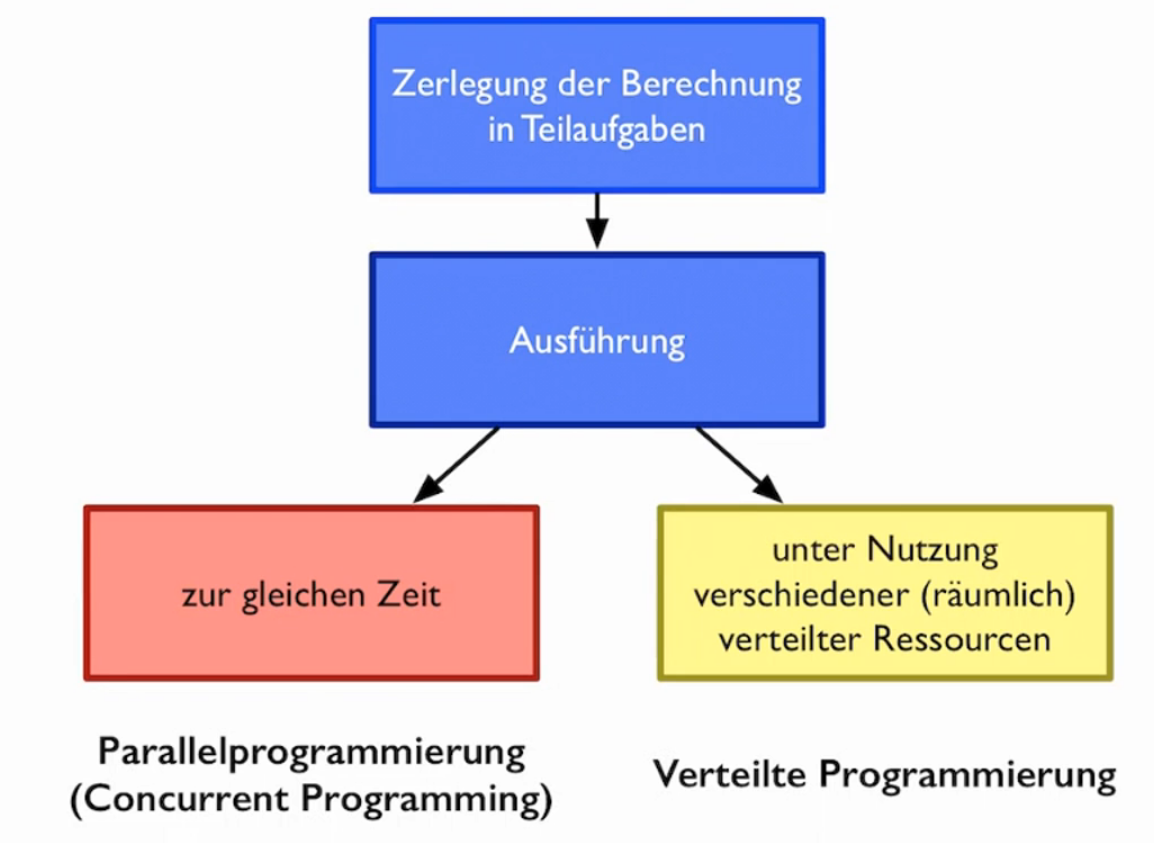
\includegraphics[width=1.0\linewidth]{Assets/Programmierparadigmen-einordnung-programmierung}
      \caption{Einordnung}
    \end{minipage}
    \hfill
    \begin{minipage}[b]{0.45\textwidth}
      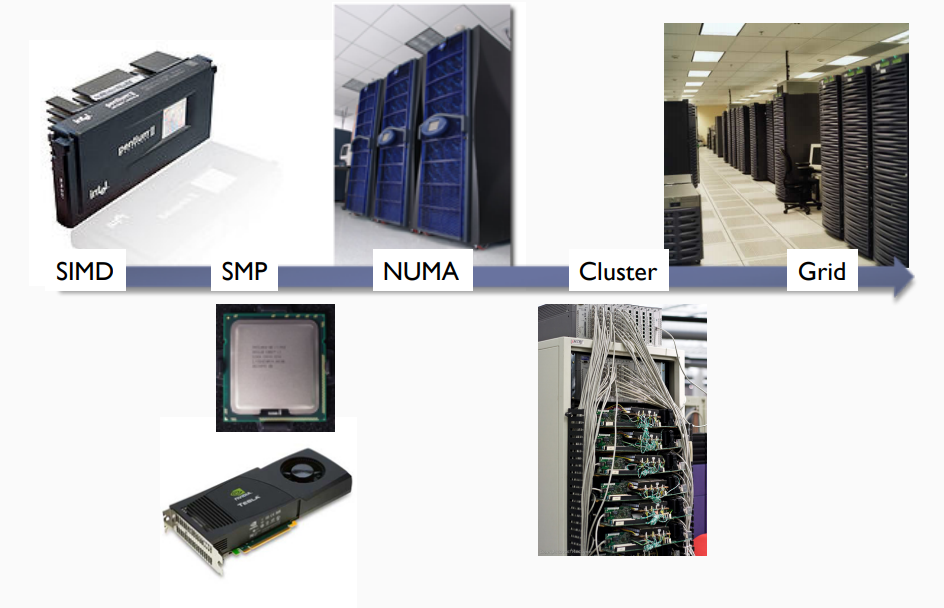
\includegraphics[width=1.0\linewidth]{Assets/Programmierparadigmen-Architekturen}
      \caption{Architekturen: SIMD, SMP, NUMA, Cluster, Grid}
    \end{minipage}
    \vfill
    \begin{minipage}[b]{0.45\textwidth}
      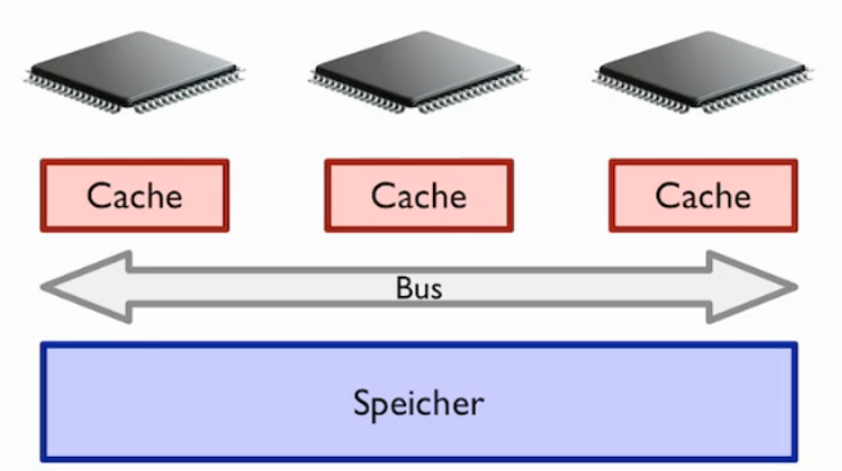
\includegraphics[width=1.0\linewidth]{Assets/Programmierparadigmen-Multiprozessorsysteme}
      \caption{Multiprozessorsysteme}
      \begin{itemize*}
        \item Zugriff über Bus auf gemeinsamen Speicher
        \item jeder Prozessor mit eigenen Caches
      \end{itemize*}
    \end{minipage}
    \hfill
    \begin{minipage}[b]{0.45\textwidth}
      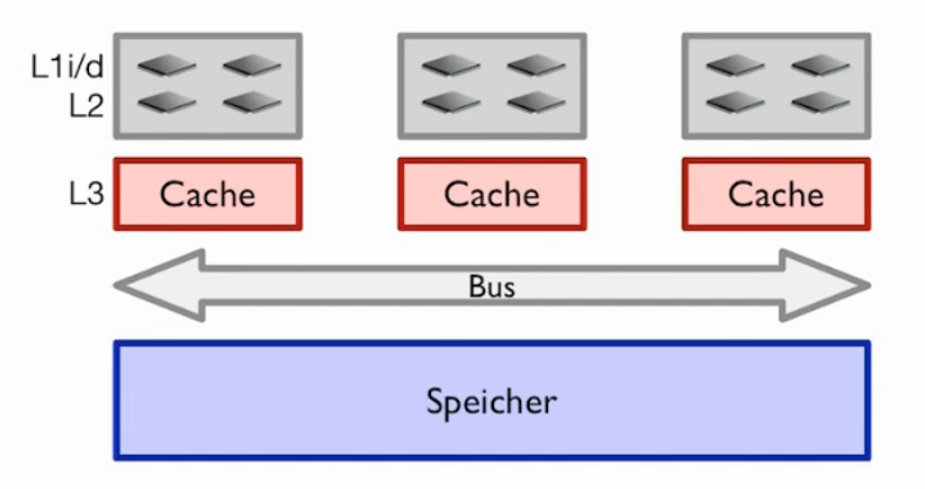
\includegraphics[width=1.0\linewidth]{Assets/Programmierparadigmen-Multicore-Systeme}
      \caption{Multicore-Systeme}
      \begin{itemize*}
        \item mehrere Prozessorkerne auf einem Chip
        \item Kerne typischerweise mit eigenen L1/L2-Caches und gemeinsamen L3-Cache
      \end{itemize*}
    \end{minipage}
    \vfill
    \begin{minipage}[b]{0.45\textwidth}
      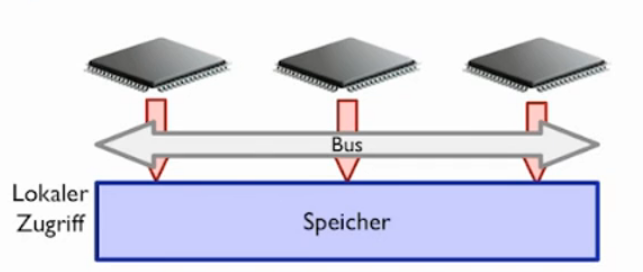
\includegraphics[width=1.0\linewidth]{Assets/Programmierparadigmen-SMP}
      \caption{SMP (Symmetric Multi Processing)}
      \begin{itemize*}
        \item Speicherbandbreite begrenzt und von allen Prozessoren gemeinsam genutzt
        \item Skalierbarkeit begrenzt
        \item Single Socket Lösung
      \end{itemize*}
    \end{minipage}
    \hfill
    \begin{minipage}[b]{0.45\textwidth}
      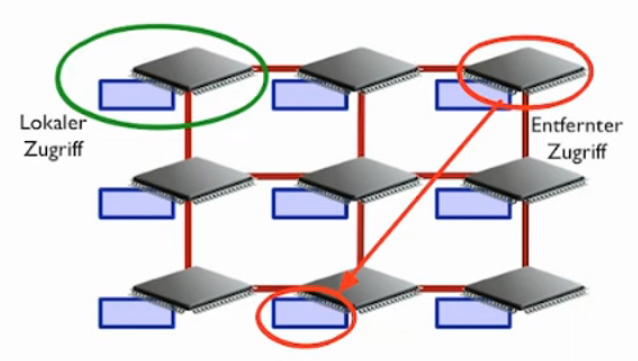
\includegraphics[width=1.0\linewidth]{Assets/Programmierparadigmen-NUMA}
      \caption{NUMA (Non-Uniform Memory Access)}
      \begin{itemize*}
        \item jedem Prozessor sind Teile des Speichers zugeordnet
        \item lokaler Zugriff ist schneller als entfernter
        \item Typisch für Multi-Socket Systeme
      \end{itemize*}
    \end{minipage}
  \end{figure}
  
  \subsubsection{Symmetrisch vs. Nicht-symmetrisch}
  \begin{tabular}{c | c}
    SMP (Symmetric Multi Processing)                                        & NUMA (Non-Uniform Memory-Access)                    \\
    Speicherbandbreite begrenzt und von allen Prozessoren gemeinsam genutzt & jedem Prozessor sind Teile des Speichers zugeordnet \\
    Skalierbarkeit begrenzt                                                 & lokaler Zugriff ist schneller als entfernter        \\
    Single Socket-Lösung                                                    & Mehr-Socket-Board                                   \\
  \end{tabular}
  
  \subsubsection{CPU vs. GPU}
  \begin{itemize*}
    \item GPU = Graphics Processing Units
    \item Hochparallele Prozessorarchitekturen (nicht nur) für Grafikrendering
  \end{itemize*}
  \begin{center}
    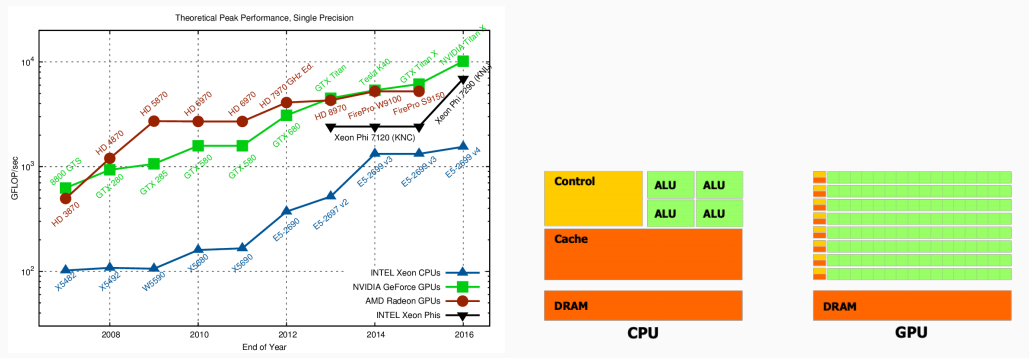
\includegraphics[width=0.95\linewidth]{Assets/Programmierparadigmen-CPU-vs-GPU}
  \end{center}
  
  \subsubsection{Flynn's Architekturklassifikation}
  \begin{center}
    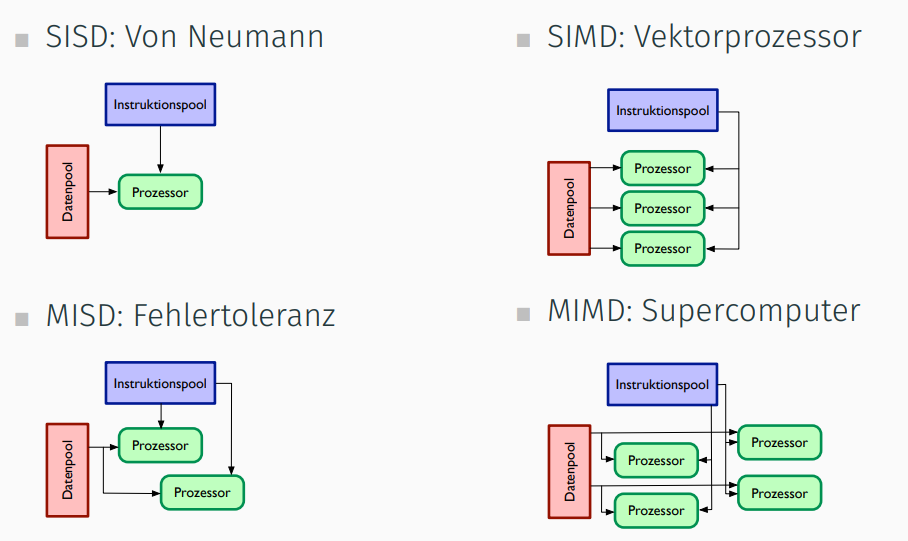
\includegraphics[width=0.95\linewidth]{Assets/Programmierparadigmen-flynn-architekturklassifikation}
  \end{center}
  
  \subsubsection{Maße zur Leistungsbewertung}
  \begin{itemize*}
    \item Maße für Laufzeitgewinn durch Parallelisierung
    \item $T_n$ = Laufzeit des Programms mit n Prozessoren/Kernen
    \item Speedup $Speedup = \frac{T_1}{T_n}$
    \item Effizienz $Effizienz =	\frac{Speedup}{n}$
  \end{itemize*}
  
  \subsubsection{Amdahlsches Gesetz}
  \begin{itemize*}
    \item Berücksichtigung parallelisierbarer und serieller Anteile im Programmablauf
    \item p = paralleler Anteil
    \item s = serieller Anteil
    \item n Prozessoren
    \item $p+s = 1$
    \item Maximaler Speedup $Speedup_{max} = \frac{T_1}{T_n} = {\frac{s+p}{s+ \frac{p}{n}}} = \frac{1}{s+\frac{p}{n}}$
  \end{itemize*}
  \begin{center}
    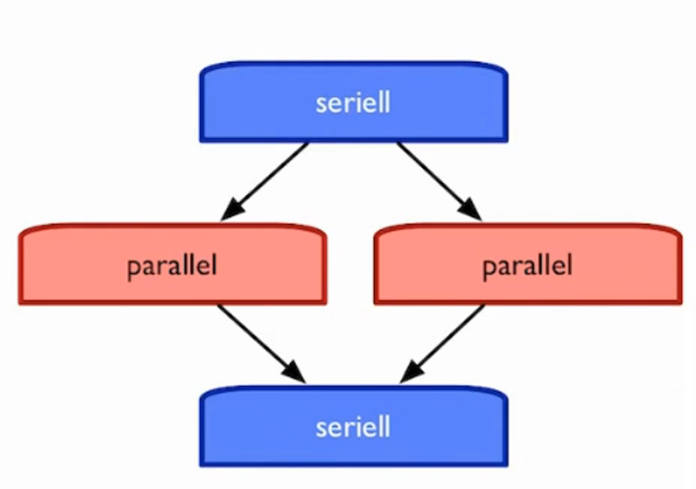
\includegraphics[width=0.35\linewidth]{Assets/Programmierparadigmen-parallelisierung}
    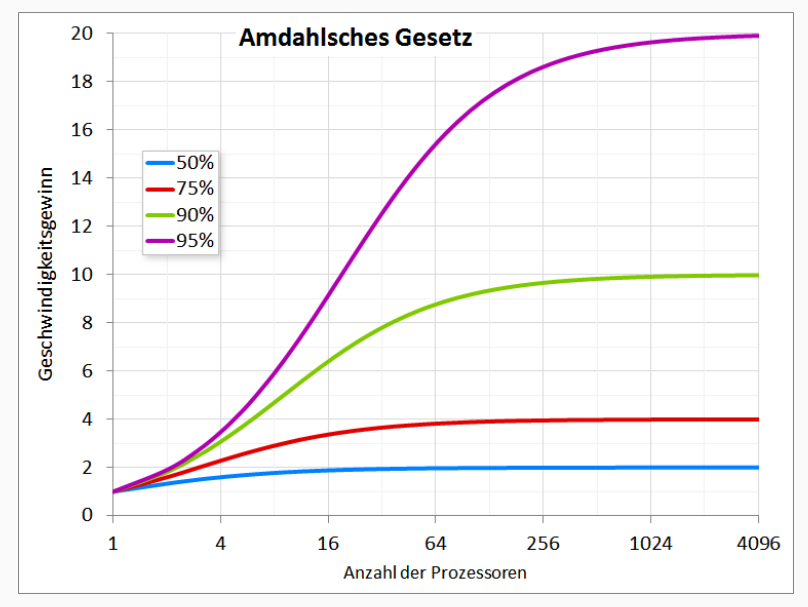
\includegraphics[width=0.35\linewidth]{Assets/Programmierparadigmen-amdahlsches-gesetz}
  \end{center}
  
  \subsubsection{Prozesse und Threads}
  Prozess := Programm in Ausführung; Ausführungsumgebung für ein Programm
  \begin{itemize*}
    \item hat eigenen Adressraum
    \item Prozessor kann immer nur einen Prozess ausführen
  \end{itemize*}
  Thread ('Faden') := leichtgewichtige Ausführungsreinheit oder Kontrollfluss (Folge von Anweisungen) innerhalb eines sich in Ausführung befindlichen Programms
  \begin{itemize*}
    \item leichtgewichtig im Vergleich zu Betriebssystemprozess
    \item Threads eines Prozesses teilen sich den Adressraum
    \item Thread kann von einer CPU oder einem Core ausgeführt werden
  \end{itemize*}
  
  \subsubsection{Shared Memory vs Message Passing}
  Art der Kommunikation zwischen Prozessen oder Threads
  \paragraph{Shared Memory}
  \begin{itemize*}
    \item Kommunikation (über Variable im) gemeinsamen Speicher
    \item Prozess kann direkt auf Speicher eines anderen Prozesses zugreifen
    \item erfordert explizite Synchronisation, z.B. über zeitkritische Abschnitte
  \end{itemize*}
  \paragraph{Message Passing}
  \begin{itemize*}
    \item Prozesse mit getrennten Adressräumen; Zugriff nur auf eigenen Speicher
    \item Kommunikation durch explizites Senden/Empfangen von Nachrichten
  \end{itemize*}
  
  \begin{figure}[!tbp]
    \centering
    \begin{minipage}[b]{0.45\textwidth}
      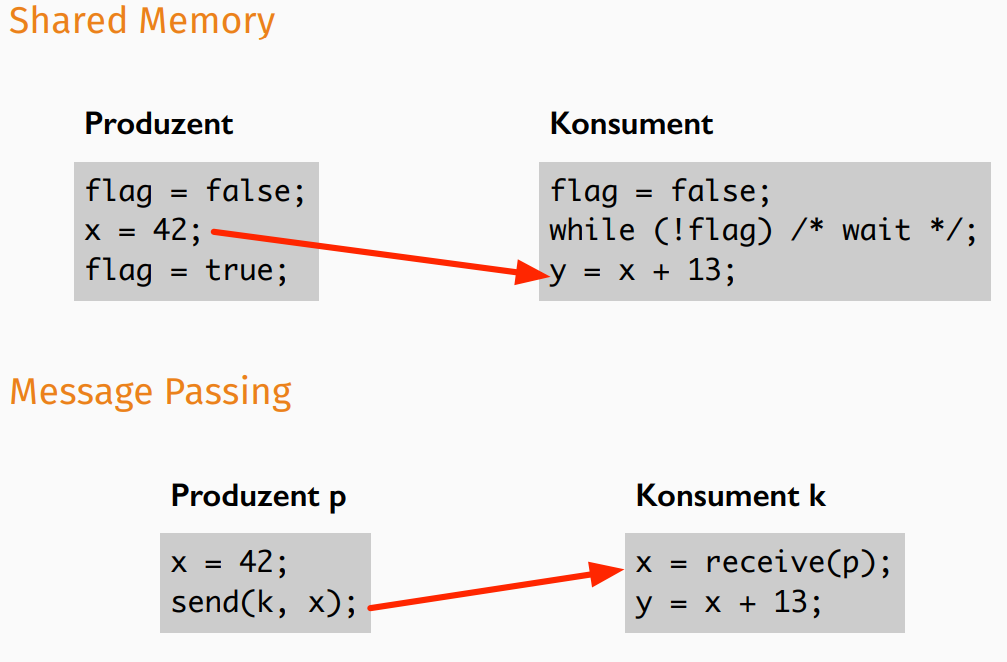
\includegraphics[width=0.4\linewidth]{Assets/Programmierparadigmen-Shared-Memory-vs-Message-Passing}
      \caption{Shared Memory vs Message Passing}
    \end{minipage}
    \hfill
    \begin{minipage}[b]{0.45\textwidth}
      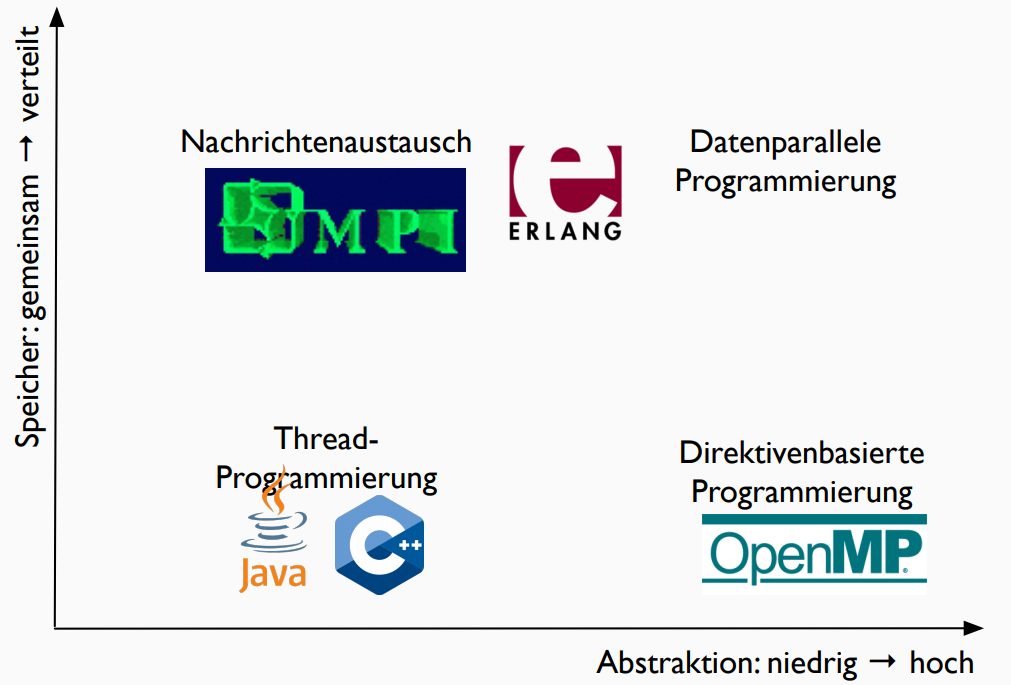
\includegraphics[width=0.9\linewidth]{Assets/Programmierparadigmen-Programmiermodelle}
      \caption{Programmiermodelle}
    \end{minipage}
  \end{figure}
  
  \subsubsection{Parallelisierungsarten}
  Instruktionsparallelität:	
  \begin{description*}
    \item[parallele Ausführung] mehrerer Operationen durch eine CPU-Instruktion
    \item[explizit] Vektorinstruktionen, SIMD
    \item[implizit] Pipelining von Instruktionen
    \item[Taskparallelität] Ausnutzung inhärenter Parallelität durch simultane Ausführung unabhängiger Aufgaben
    \item[Datenparalelität] \hfill
    \begin{itemize*}
      \item Gemeinsame Operation auf homogener Datenmenge
      \item Zerlegung eines Datensatzes in kleinere Abschnitte
    \end{itemize*}
  \end{description*}
  
  \begin{figure}[!tbp]
    \centering
    \begin{minipage}[b]{0.45\textwidth}
      \includegraphics[width=0.9\linewidth]{Assets/Programmierparadigmen-Instruktionsparallelität}
      \caption{Instruktionsparallelität: SIMD}
      \begin{itemize*}
        \item Autovektorisierung durch Compiler
        \item explizite Instruktionen
        \item Beispiel: Addition zweier Vektoren
      \end{itemize*}
    \end{minipage}
    \hfill
    \begin{minipage}[b]{0.45\textwidth}
      \includegraphics[width=0.4\linewidth]{Assets/Programmierparadigmen-Taskparallelität}
      \caption{Taskparallelität}
      \begin{itemize*}
        \item Unabhängikeit von Teilprozessen $\rightarrow$ Desequentialisierung
        \item Beispiel: Quicksort
      \end{itemize*}
    \end{minipage}
    \vfill
    \begin{minipage}[b]{0.45\textwidth}
      \includegraphics[width=0.9\linewidth]{Assets/Programmierparadigmen-Datenparallelität}
      \caption{Datenparallelität}
      \begin{itemize*}
        \item homogene Datenmenge: Felder, Listen, Dokumentenmenge,...
        \item Verteilung der Daten
        \item alle Prozessoren führen gleiches Programm auf jeweils eigenen Daten aus
        \item Beispiel: Matrixaddition S = A + B
      \end{itemize*}
    \end{minipage}
  \end{figure}
  
  \subsubsection{Herausforderungen}
  \begin{itemize*}
    \item Zerlegung eines Problems in parallel verarbeitbare Teile
    \begin{itemize*}
      \item Beispiel: Suche in einer Datenbank mit 1 TB Größe
      \item Annahme: 100 MB/Sekunde mit einem Prozessor = 175 Minuten
      \item bei paralleler Suche durch 10 Prozessoren = 17.5 Minuten
      \item Übertragbar auf andere Probleme, z.B. Sortieren, Suche in Graphen?
    \end{itemize*}
    \item Synchronisation konkurrierender Zugriffe auf gemeinsame Ressourcen
    \begin{itemize*}
      \item Beispiel: Produzent-Konsument-Beziehung
      \item Annahme: Datenaustausch über gemeinsame Liste
      \item Fragestellungen: Benachrichtigung über neues Element in der Liste, Konsument entnimmt Element während Produzent einfügt
      \item Wechselseitiger Ausschluss
    \end{itemize*}
    \item außerdem: Fehlersuche, Optimierung
  \end{itemize*}
  
  \subsubsection{Zusammenfassung}
  \begin{itemize*}
    \item Parallele Verarbeitung als wichtiges Paradigma moderner Software
    \item verschiedene parallele
    \begin{itemize*}
      \item Hardwarearchitekturen und
      \item Programmiermodelle
    \end{itemize*}
    \item Herausforderungen
    \begin{itemize*}
      \item Problemzerlegung
      \item Synchronisation
      \item ...
    \end{itemize*}
    \item im Weiteren: konkrete Methoden und Techniken in Erlang und C++
  \end{itemize*}
  
  \subsection{Parallele Programmierung in Erlang}
  \subsubsection{Unterstützung paralleler Programmierung in Erlang}
  \begin{itemize*}
    \item Leichtgewichtige Prozesse und Message Passing
    \item SMP-Support (Symmetric Multi Processing)
    \item Ziele für effiziente Parallelisierung
    \begin{itemize*}
      \item Problem in viele Prozesse zerlegen (aber nicht zu viele ...)
      \item Seiteneffekte vermeiden  (würde Synchronisation erfordern ...)
      \item Sequentiellen Flaschenhals vermeiden (Zugriff auf gemeinsame Ressourcen: IO, Registrierung von Prozessen, ...) -> Small Messages, Big Computation! 
    \end{itemize*}
  \end{itemize*}
  
  \subsubsection{Prozesse in Erlang}
  \begin{itemize*}
    \item Erlang VM = Betriebssystemprozess
    \item Erlang-Prozess = Thread innerhalb der Erlang VM
    \begin{itemize*}
      \item kein Zugriff auf gemeinsame Daten, daher 'Prozess'
    \end{itemize*}
    \item jede Erlang-Funktion kann einen Prozess bilden
    \item Funktion spawn erzeugt einen Prozess, der die Funktion Fun ausführt 
    \begin{lstlisting}
    Pid = spawn(fun Fun/0)
    \end{lstlisting}
    \item Resultat = Prozessidentifikation Pid, mittels der man dem Prozess Nachrichten schicken kann.
    \item über self() kann man die eigene Pid ermitteln
    \item Übergabe von Arghumenten an den Prozess bei der Erzeugung
    \begin{lstlisting}
    Pid = spawn(fun() -> any_func(Arg1, Arg2, ...) end)
    \end{lstlisting}
  \end{itemize*}
  
  \begin{figure}[!tbp]
    \centering
    \begin{minipage}[b]{0.45\textwidth}
      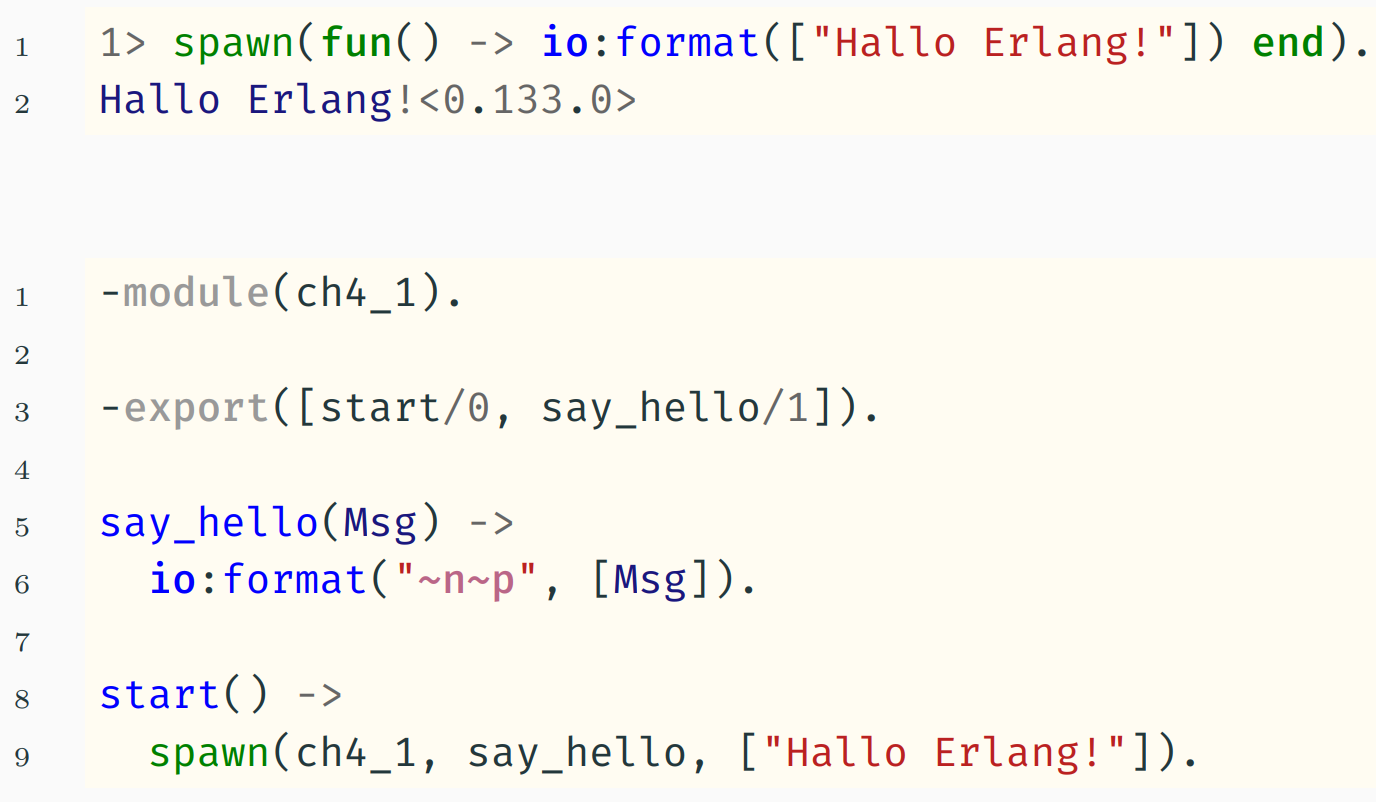
\includegraphics[width=0.9\linewidth]{Assets/Programmierparadigmen-erlang-Beispiele}
      \caption{Beispiele}
    \end{minipage}
    \hfill
    \begin{minipage}[b]{0.45\textwidth}
      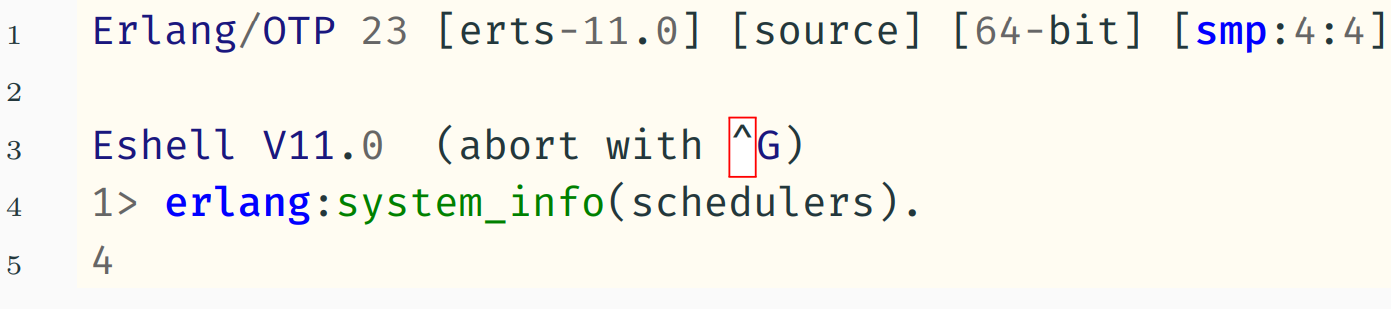
\includegraphics[width=0.4\linewidth]{Assets/Programmierparadigmen-SMP Erlang}
      \caption{SMP Erlang}
    \end{minipage}
  \end{figure}
  
  \begin{itemize*}
    \item 4 Betriebssystemthreads (hier 2 Kerne mit Hyperthreading)
    \item kann mit -smp [disable $\mid$ enable $\mid$ auto] beeinflusst werden
    \item +S [Anzahl] bestimmt Anzahl der Scheduler
    \begin{itemize*}
      \item sollte nicht größer als Anzahl der Kerne/Prozessoren sein
    \end{itemize*}
  \end{itemize*}
  
  \subsubsection{Scheduler in Erlang}
  \begin{center}
    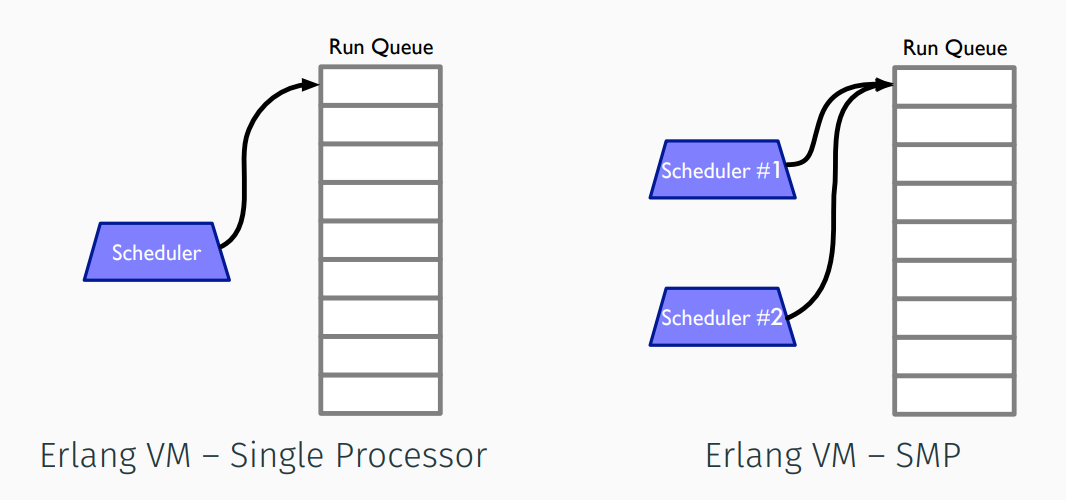
\includegraphics[width=0.4\linewidth]{Assets/Programmierparadigmen-erlang-scheduler}
  \end{center}
  
  \subsubsection{Message Passing in Erlang: Senden einer Nachricht}
  \begin{lstlisting}
  Pid ! Message
  \end{lstlisting}
  \begin{itemize*}
    \item an Prozess Pid wird die Nachricht Message gesendet
    \item der Prozess muss eine Empfangsoperation ausführen. damit ihn die Nachricht erreichen kann
    \begin{lstlisting}[language=erlang]
    receive
        Pattern1 [when Guard1] -> Expressions1;
        Pattern2 [when Guard2] -> Expressions2;
        ...
    end
    \end{lstlisting}
    \item trifft eine Nachricht ein, wird versucht, diese mit einem Pattern und ggf. vorhandenen Guard zu 'matchen'
    \item erstes zutreffendes Pattern (inkl. Guard) bestimmt, welcher Ausdruck ausgewertet wird
    \item trifft kein Pattern zu, wird die Nachricht für spätere Verwendung aufgehoben und Prozess wartet auf die nächste Nachricht ($\rightarrow$ selective receive)
  \end{itemize*}
  
  
  \subsubsection{Ein einfacher Echo-Server}
  \begin{lstlisting}[language=erlang]
-module(ch4_2).
-export([run/0]).

run() -> Pid2 = spawn(fun loop/0),
  Pid2 ! {self(), hellp},
  receive
    {Pid2, Msg} -> io:format("P1 ~w~n", [Msg])
  end,
  Pid2 ! stop.

loop() ->
  receive
    {From, Msg} -> From ! {self(), Msg}, loop();
    stop -> true
  end.
\end{lstlisting}
  
  Erklärungen
  \begin{itemize*}
    \item Funktion loop() realisiert einen (nur bedingt nützlichen) Echo-Dienst, der jede empfangene Nachricht unverändert an den Absender zurückschickt, bis er nach Empfang von stop endet
    \item Funktion run()
    \begin{enumerate*}
      \item startet den Echoserver (Zeile 4)
      \item schickt ihm als nächstes eine Nachricht (Zeile 5)
      \item wartet auf eine Antwort (Zeile 6)
      \item gibt diese aus (Zeile 7)
      \item schickt dann stop an den Echoserver (Zeile 9)
    \end{enumerate*}
    \item Aufruf in der Funktion loop() erfolgt endrekursiv, daher wird kein wachsender Aufrufstapel angelegt (Hinweis: grundsätzlich zu beachten, da sonst der Speicherbedarf stetig wächst)
  \end{itemize*}
  
  \subsubsection{Ansätze zur Parallelisierung}
  \begin{itemize*}
    \item Beispiel: Berechnung einer (zufällig generierten) Liste von Fibonaccizahlen
    \item Sequentielle Lösung über lists:map/2
  \end{itemize*}
  \begin{lstlisting}[language=erlang]
% Berechnung der Fibonacci Zahl für F
fibo(0) -> 0;
fibo(1) -> 1;
fibo(F) when F > 0 -> fibo(F-1) + fibo(F-2).

% Liste von Num Fibonacci Zahlen
run(Num) ->
  Seq = list:seq(1, Num), %Zufallszahlen erzeugen
  Data = lists:map(fun(_) -> random:uniform(20) end, Seq),
  lists:map(fun fibo/1, Data)
\end{lstlisting}
  
  \subsubsection{pmap: Parallele Funktionen höherer Ordnung}
  \begin{itemize*}
    \item Parallele Variante von lists:map(Fun, list)
    \item für jedes Listenelement einen Prozess erzeugen
    \item Ergebnisse einsammeln
  \end{itemize*}
  \begin{lstlisting}[language=erlang]
pmap(F, L) ->
  S = self(), % Berechnung der Fibonacci Zahl für F
  Pids = lists:map(fun(I) ->
      % Prozess erzeugen
      spawn(fun() -> do_fun(S, F, I) end)
    end, L), % Ergebnisse einsammeln
    gather(Pids).
\end{lstlisting}
  
  \paragraph{pmap: Hilfsfunktionen}
  
  \color{orange} Eigentliche Verarbeitungsfunktion ausführen \color{black}
  \begin{lstlisting}[language=erlang]
do_fun(Parent, F, I) ->
  % Parent ist der Elternprozess
  Parent ! { self(), (catch F(I))}.
\end{lstlisting}
  \begin{itemize*}
    \item Funktion F aufrufen, catch sorgt für korrekte Behandlung von Fehlern in F
    \item Ergebnis zusammen mit eigener Pid (self()) an Elternprozess senden
  \end{itemize*}
  
  \color{orange} Einsammeln der Ergebnisse \color{black}
  \begin{lstlisting}[language=erlang]
gather([Pid | T]) ->
  receive
  % Ordnung der Ergebnisse entspricht Ordnung der Argumente
    { Pid, Ret } -> [Ret | gather(T)]
  end;
gather([]) -> [].
\end{lstlisting}
  \begin{itemize*}
    \item Zeile 5: Warten bis Paar (Pid, Ergebniswert) eintrifft
    \item Zeile 7: Tail ist leer $\rightarrow$ alle Ergebnisse eingetroffen
  \end{itemize*}
  
  \paragraph{Parallele Berechnung der Fibonacci-Zahlen}
  \begin{lstlisting}[language=erlang]
%Liste von Num Fibonacci Zahlen
run(Num) ->
  Seq = lists:seq(1, Num), % Zufallszahlen erzeugen
  Data = lists:map(fun(_) -> random:uniform(20) end, Seq),
  % Berechnung parallel ausführen
  pmap(fun fibo/1, Data).
\end{lstlisting}
  
  \paragraph{Diskussion}
  
  \begin{itemize*}
    \item Passende Abstraktion wählen
    \begin{itemize*}
      \item Ist Ordnung der Ergebnisse notwendig?
      \item Werden Ergebnisse benötigt?
    \end{itemize*}
    \item Anzahl der parallelen Prozesse
    \begin{itemize*}
      \item Abhängig von Berechnungsmodell, Hardware etc.
      \item evtl. pmap mit max. Anzahl gleichzeitiger Prozesse
    \end{itemize*}
    \item Berechnungsaufwand der Prozesse
    \begin{itemize*}
      \item Berechnung vs. Daten/Ergebnisse senden
    \end{itemize*}
  \end{itemize*}
  
  \paragraph{pmap: Alternative Implementierung}
  
  \begin{itemize*}
    \item ohne Berücksichtigung der Ordnung der Ergebnismenge
    \item Zählen für die bereits eingetroffenen Ergebnisse
  \end{itemize*}
  \begin{lstlisting}[language=erlang]
  pmap(F, L) ->
    ...
    gather2(length(L), Ref, []).
  
  gather2(N, Ref, L) ->
    receive
      {Ref, Ret} -> gather2(N-1, Ref, [Ret | L ])
    end;
  gather2(0,_, L) -> L.
\end{lstlisting}
  
  \subsubsection{Speedup}
  Bestimmung des Speedups erfordert
  \begin{itemize*}
    \item Zeitmessung
    \item Kontrolle der genutzten Prozessoren/Cores
  \end{itemize*}
  \color{orange} Welchen Einfluss hat die Zahl der erzeugten Prozesse. \color{black}
  
  \paragraph{Speedup: Zeitmessung}
  
  Nutzung der Funktion timer:tc/3
  \begin{lstlisting}
> timer:tc(ch4_4, run, [30]).
{7900,[233,1,987,610,377,8,144,89,89,3]}
\end{lstlisting}
  Für bessere Aussagekraft: mehrfache Ausführung
  \begin{lstlisting}[language=erlang]
benchmark(M, Fun, D) ->
  % 100 Funktionsaufrufe
  Runs = [timer:tc(M, Fun, [D]) || _ <- lists:seq(1, 100)],
  % Durchschnitt der Laufzeiten in Millisekunden berechnen
  lists:sum([T || {T, _ } <- Runs]) / (1000 * length(Runs)).
\end{lstlisting}
  
  \paragraph{Bestimmung: Speedup}
  
  ch4\_6:benchmark(ch4\_4, run, 1000).
  \begin{center}
    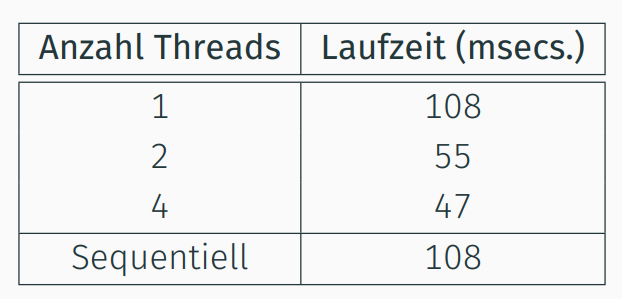
\includegraphics[width=0.4\linewidth]{Assets/Programmierparadigmen-Speedup-Bestimmung}
  \end{center}
  \color{orange} Achtung: \color{black}
  \begin{itemize*}
    \item Aufwand für Berechnung einer Fibonaccizahl ist nicht konstant
    \item Zufallszahlen als Eingabe
  \end{itemize*}
  
  \paragraph{Diskussion: Speedup}
  
  \begin{center}
    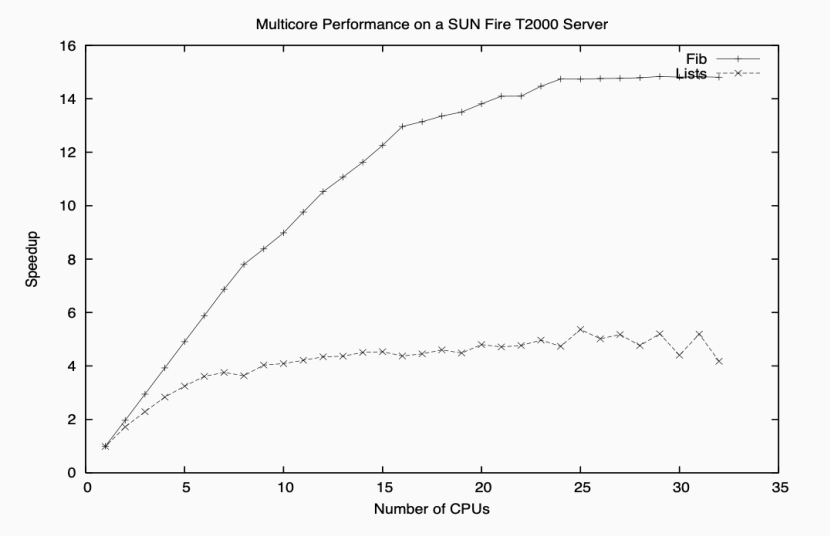
\includegraphics[width=0.4\linewidth]{Assets/Programmierparadigmen-Speedup-Diskussion}
  \end{center}
  
  \subsubsection{Datenparallelität: Das Map-Reduce-Paradigma}
  \begin{itemize*}
    \item Parallelisierungsmuster inspiriert von Konzepten funktionaler Programmiersprachen (map,reduce/fold)
    \item Basis von Big-Data-plattformen wie Hadoop, Spark,...
    \item Grundidee:
    \begin{itemize*}
      \item map(F, Seq) ? wende Funktion F (als Argument übergeben) auf alle Elemente einer Folge Seq an,
      \begin{itemize*}
        \item Funktion F kann unabhängig (=parallel) auf jedes Element angewendet werden
        \item Partitionieren und Verteilen der Elemente der Folge
        \item z.B. multipliziere jedes Element mit 2
      \end{itemize*}
      \item reduce(F, Seq) = wende eine Funktion F schrittweise auf die Elemente einer Folge Seq an und produziere einen einzelnen Wert,
      \begin{itemize*}
        \item prinzipiell ähnlich zu map(F, Seq), d.h. Funktion F kann auf Paare unabhängig angewendet werden
        \item z.B. die Summe aller Elemente der Folge
      \end{itemize*}
    \end{itemize*}
  \end{itemize*}
  
  \paragraph{map in Erlang}
  
  \begin{center}
    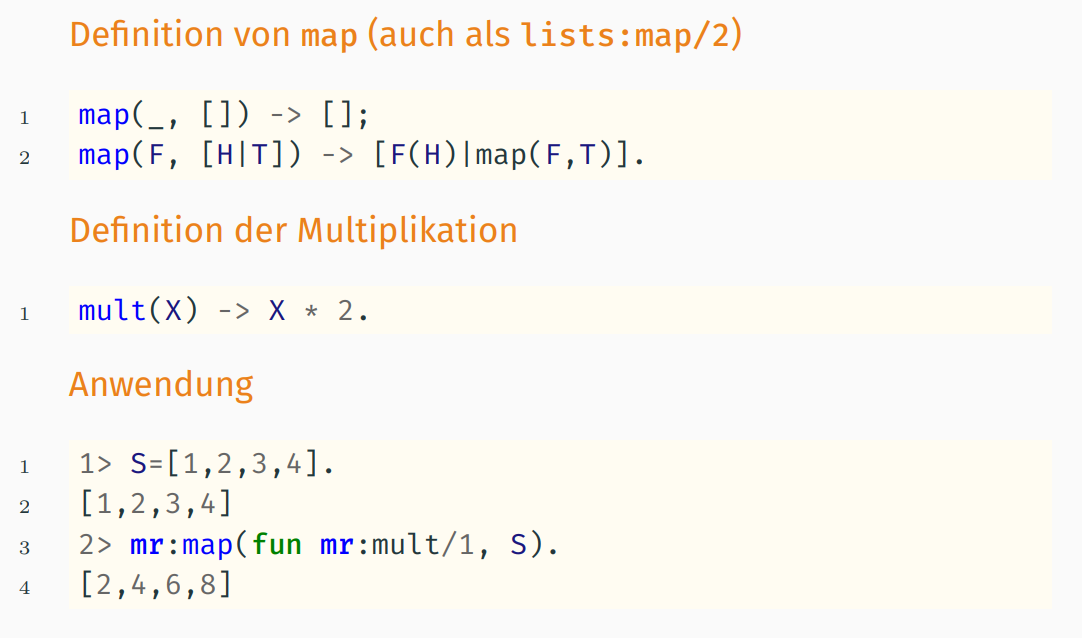
\includegraphics[width=0.4\linewidth]{Assets/Programmierparadigmen-erlang-map}
  \end{center}
  
  \paragraph{reduce in Erlang}
  
  \begin{center}
    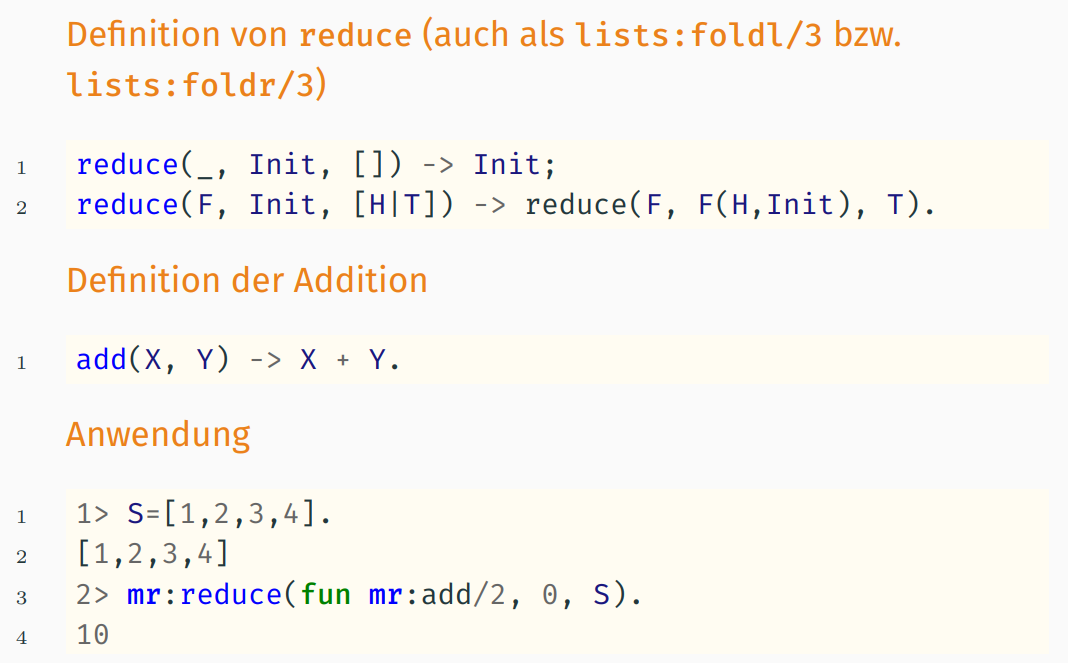
\includegraphics[width=0.4\linewidth]{Assets/Programmierparadigmen-erlang-reduce}
  \end{center}
  
  \paragraph{Parallelisierung von map und reduce}
  
  \color{orange} map \color{black}
  \begin{itemize*}
    \item Funktion F kann unabhängig (=parallel) auf jedes Element angewendet werden
    \item Partitionieren und Verteilen der Elemente der Folge
    \item siehe pmap
  \end{itemize*}
  \color{orange} reduce \color{black}
  \begin{itemize*}
    \item prinzipiell ähnlich, d.h. Funktion F kann auf Paare unabhängig angewandt werden
  \end{itemize*}
  
  \paragraph{Parallelisierung von reduce}
  
  \begin{center}
    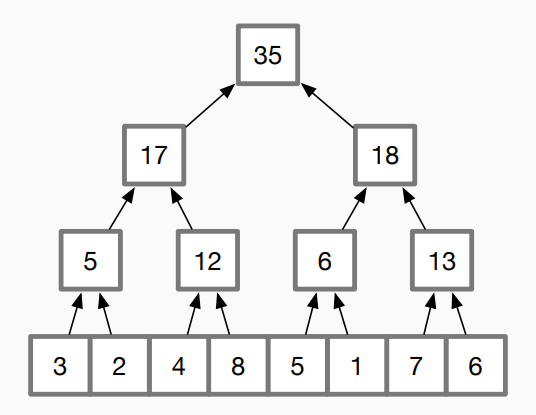
\includegraphics[width=0.5\linewidth]{Assets/Programmierparadigmen-erlang-reduce-parallel}
  \end{center}
  
  \subsubsection{Taskparallelität: Sortieren}
  \color{orange} Quicksort in Erlang \color{black}
  \begin{lstlisting}[language=erlang]
qsort([]) -> [];
qsort([H|T]) -> qsort([Y || Y <- T, Y < H]) ++
    [H] ++
    qsort([Y || Y <- T, Y >= H]).
\end{lstlisting}
  
  \begin{itemize*}
    \item typische funktionale Notation von Quicksort mit List Comprehensions
    \item Zeile 2: H dient als Pivotelement
  \end{itemize*}
  Idee:
  \begin{itemize*}
    \item Prozess für das Sortieren der einen Hälfte starten
    \item Elternprozess kann andere Hälfte sortieren
    \item rekursive Zerlegung...
  \end{itemize*}
  
  \subsubsection{Parallel Quicksort}
  \paragraph{Version 1}
  
  Quicksort in Erlang
  \begin{lstlisting}[language=erlang]
qsort2([]) -> [];
qsort2([H|T]) ->
  Parent = self(),
  spawn(fun() ->
    Parent ! qsort2([X || X <- T, X >= H]) end),
  qsort2([Y || Y <- T, Y < H]) ++
      [H] ++
      receive T2 -> T2 end.
\end{lstlisting}
  
  Erläuterungen
  \begin{itemize*}
    \item Zeile 4: Erzeugen eines neuen Prozesses zur Sortierung der 'oberen' Hälfte
    \item Zeile 6-7: Wie bisher
    \item Zeile 8: Warten auf Empfang der sortierten anderen Hälfte
  \end{itemize*}
  Zeitmessung:
  \begin{lstlisting}
> L = ch4_6:rand_list(100000).
...
> ch4_6:benchmark(ch4_10, qsort, L).
131.90963
> ch4_6:benchmark(ch4_10, qsort2, L).
293.59211
\end{lstlisting}
  
  Bewertung
  \begin{itemize*}
    \item parallele Version 1 ist langsamer!
    \item mögliche Erklärung: Prozess-Start ist aufwändiger als Sortieren kleiner Teilfolgen
    \item bessere Variante nach John Hughes: Parallel Programming in Erlang
    \begin{itemize*}
      \item Kontrolle der Granularität für parallele Ausführungen
      \item danach Sortieren mit sequenzieller Variante
      \item einfache Idee: Anzahl der parallelen Zerlegung begrenzen
    \end{itemize*}
  \end{itemize*}
  \begin{lstlisting}[language=erlang]
qsort3(L) -> qsort3(4, L). % 4 Rekursionsstufen parallel

qsort3(0, L) -> qsort(L); % Umschalten
\end{lstlisting}
  
  \paragraph{Version 2}
  \begin{lstlisting}[language=erlang]
qsort3(L) -> qsort3(6, L).

qsort3(0, L) -> qsort(L);
qsort3(_, []) -> [];
qsort3(N, [H|T]) ->
  Parent = self(), spawn_link(fun() ->
    Parent ! qsort3(N-1, [Y || Y <- T, Y >= H])
  end),
qsort3(N-1, [Y || Y <- T, Y < H]) ++
    [H] ++
    receive T2 -> T2 end.  
\end{lstlisting}
  \begin{lstlisting}
> ch4_6:benchmark(ch4_10, qsort3, L).
87.54315
\end{lstlisting}
  
  \subsubsection{Fazit}
  \begin{itemize*}
    \item \color{orange} leichtgewichtige Prozesse \color{black} als Baustein der Parallelisierung in Erlang
    \item Prozesskommunikation ausschließlich über \color{orange} Message Passing \color{black}
    \item \color{orange} funktionaler Charakter \color{black} (u.a. Vermeidung von Seiteneffekten) vereinfacht Parallelisierung deutlich
    \item \color{orange} Daten- und Taskparallelität \color{black} möglich
    \item hoher Abstraktionsgrad, aber auch wenig Einflussmöglichkeiten
  \end{itemize*}
  
  \subsection{Parallele Programmierung in C++}
  \subsubsection{Threads in C++}
  \color{orange} Thread (Faden) \color{black} = leichtgewichtige Ausführungseinheit oder Kontrollfluss (Folge von Anweisungen) innerhalb eines sich in Ausführung befindlichen Programms 
  \begin{itemize*}
    \item Threads teilen sich den Adressraum ihres Prozesses
    \item in C++: Instanzen der Klasse std::thread
    \item führen eine (initiale) Funktion aus
  \end{itemize*}
  \begin{lstlisting}[language=C++]
  #include <thread>
  #include <iostream>

  void say_hello() {
    std::cout << "Hello Concurrent C++\n";
  }

  int main() {
    std::thread t(say_hello);
    t.join();
  }
  \end{lstlisting}
  
  \paragraph{Alternative Erzeugung von Threads}
  
  \color{orange} über Lambda-Ausdruck \color{black}
  \begin{lstlisting}[language=C++]
  std::thread t([]() { do_something(); });
  \end{lstlisting}
  
  \color{orange} mit Instanzen einer Klasse \color{black} - erfordert Überladen von operator()
  \begin{lstlisting}[language=C++]
  struct my_task {
    void operator()() const { do_something(); }
  };

  my_task tsk;
  std::thread t1(tsk); // mit Objekt
  std::thread t2{ my_task() }; // über Konstruktor
  \end{lstlisting}
  
  \paragraph{Parameterübergabe bei Threaderzeugung}
  
  \begin{itemize*}
    \item über zusätzliche Argumente des thread-Konstruktors
    \item Vorsicht bei Übergabe von Referenzen, wenn Elternthread vor dem erzeugten Thread beendet wird
  \end{itemize*}
  \begin{lstlisting}[language=C++]
  void fun(int n, const std::string& s) {
      for (auto i = 0; i < n; i++)
          std::cout << s << " ";
      std::cout << std::endl;
  }
  std::thread t(fun, 2, "Hello");
  t.join();
  \end{lstlisting}
  
  \paragraph{Warten auf Threads}
  
  \begin{itemize*}
    \item t.join() wartet auf Beendigung des Threads t
    \item blockiert aktuellen Thread
    \item ohne join() keine Garantie, dass t zur Ausführung kommt
    \item Freigabe der Ressourcen des Threads
  \end{itemize*}
  \begin{lstlisting}[language=C++]
  std::thread t([]() { do_something(); });
  t.join();
\end{lstlisting}
  \begin{lstlisting}[language=C++]
// Erscheint die Ausgabe?
#include <iostream>
#include <thread>
#include <chrono>

int main() {
  std::thread t([]() {
    std::this_thread::sleep_for( std::chrono::seconds(1) );
    std::cout << "Hello\n";
  });
}
\end{lstlisting}
  
  \paragraph{Hintergrundthreads}
  
  \begin{itemize*}
    \item Threads können auch im Hintergrund laufen, ohne, dass auf Ende gewartet werden muss
    \item 'abkoppeln' durch detach()
    \item Thread läuft danach unter Kontrolle des C++-Laufzeitsystems, join nicht mehr möglich
  \end{itemize*}
  
  \paragraph{Threadidentifikation}
  
  \begin{itemize*}
    \item Threadidentifikator vom Typ std::thread::id
    \item Ermittlung über Methode get\_id()
  \end{itemize*}
  \begin{lstlisting}[language=C++]
  void fun() {
  std::cout << "Hello from "
            << std::this_thread::get_id()
            << std::endl;
  }
  std::thread t(fun);
  t.join();
  \end{lstlisting}
  
  \paragraph{Beispiel: Berechnung von Fibonacci-Zahlen in C++}
  \begin{itemize*}
    \item rekursive und nichtrekursive Variante möglich
  \end{itemize*}
  \begin{lstlisting}[language=C++]
unsigned int fibonacci(unsigned int n) {
  if(n == 0)
    return 0;

  unsigned int f0 = 0, f1 = 1, f2;
  for(auto i=1u; i<n; i++){
    f2 = f0 + f1;
    f0 = f1;
    f1 = f2;
  }
  return f1;
}
\end{lstlisting}
  
  Parallele Berechnung von Fibonacci-Zahlen
  \begin{itemize*}
    \item einfachste Lösung (ähnlich zu Erlang): pro Zahl ein Thread
  \end{itemize*}
  \begin{lstlisting}[language=C++]
std::vector<std::thread> threads;
unsigned int results[20];

for (auto i = 0u; i<20; i++){
  auto f = rand() % 30;
  threads-push_back(std::thread([&](){
    results[i] = fibonacci(f);
  }));
}
std::for_each(threads.begin(), threads.end(), std::mem_fn(&std::thread::join));
\end{lstlisting}
  
  Erläuterungen
  \begin{itemize*}
    \item Zeile 1: Feld der Threads
    \item Zeile 2: Feld für Ergebniswerte
    \item Zeile 5: Zufallszahl erzeugen
    \item Zeilen 6-7 Thread zur Berechnung der Fibonacci-Zahl erzeugen und Ergebnis im Feld speichern
    \item Zeile 10-11: Warten auf Beendigung der Threads (std::mem\_fn = Wrapper für Zeiger auf Member-Funktion)
    \item \color{orange} aber: \color{black}
    \begin{itemize*}
      \item Zugriff auf gemeinsame Ressource (results)!
      \item Anzahl Fibonaccizahlen = Anzahl Threads
    \end{itemize*}
  \end{itemize*}
  
  \paragraph{parallel-for in C++}
  
  \begin{itemize*}
    \item Unterstützung durch Higher-Level-APIs und Frameworks
  \end{itemize*}
  \begin{lstlisting}[language=C++]
// OpenMP
#pragma omp parallel for
  for(auto i=0u; i<n; i++){...}

// Parallele Algorithmen in C++17
std::for_each(std::execution::par_unseq, vec.begin(), vec.end(), [](auto&& item) {...});

// Intel TBB
tbb::parallel_for(tbb::blocked_range<int>(0, vec.size()), [&](tbb::blocked_range<int> r){...});
\end{lstlisting}
  
  \paragraph{Kontrolle der Anzahl der Threads}
  
  \begin{itemize*}
    \item Erzeugung von Threads ist mit Kosten verbunden
    \item begrenzte Anzahl von Hardwarethreads (Anzahl Cores, Hyperthreading)
    \item Ermittlung der Anzahl der unterstützten Hardwarethreads
  \end{itemize*}
  \begin{lstlisting}[language=C++]
std::thread::hardware_concurrency()
\end{lstlisting}
  \begin{itemize*}
    \item Nutzung für Implementierung von Threadpools, Task Libraries, ...
  \end{itemize*}
  
  \subsubsection{Probleme nebenläufiger Ausführung}
  \begin{lstlisting}[language=C++]
struct jawsmith {
  std::string msg;
  
  jawsmith(const std::string& m) : msg(m) {}
  void operator()() const {
    for(;;){
      std::this_thread::sleep_for( std::chrono::seconds(1) );
      for(auto& c: msg) {
        std::cout << c << std::flush;
      }
    }
  }
}
\end{lstlisting}
  \begin{lstlisting}[language=C++]
std::thread t1 { jawsmith("DASISTEINELANGENACHRICHT)};
std::thread t2 { jawsmith("dieistaberauchnichtkurz)};
\end{lstlisting}
  Ausgabe:
  \begin{lstlisting}[language=C++]
dDieistaberauchnichtkASISTEINELANGENACHurzRICHT...
\end{lstlisting}
  
  \color{orange} Race Conditions \color{black}(Wettlaufsituationen) := Ergebnis nebenläufiger Ausführung auf gemeinsamen Zustand (hier: Ausgabekanal) hängt vom zeitlichen Verhalten der Einzeloperationen ab
  
  
  \begin{itemize*}
    \item Race Conditions (Wettlaufsituation) := Ergebnis nebenläufiger Ausführung auf gemeinsamen Zustand (hier: Ausgabekanal) hängt vom zeitlichen Verhalten der Einzeloperationen ab
    \item kritischer Abschnitt: Programmabschnitt in einem Thread, in dem auf eine gemeinsame Ressource (Speicher etc.) zugegriffen wird und der nicht parallel (oder zeitlich verzahnt) zu einem anderen Thread ausgeführt werden darf
    \item Lösung durch wechselseitigen Ausschluss (engl. mutual exclusion = mutex)
    \begin{itemize*}
      \item Instanz der Klasse std::mutex
      \item Methoden zum Sperren ( lock ) und Freigeben ( unlock )
      \item 'mutex' : Standard-Mutex für exklusiven Zugriff
      \item 'timed\_mutex' : Mutex mit Timeout für Warten ( try\_lock\_for() )
      \item 'recursive\_mutex' : rekursives Mutex - erlaubt mehrfaches Sperren durch einen Thread, z.B. für rekursive Aufrufe
      \item 'recursive\_timed\_mutex' : rekursives Mutex mit Timeout
      \item 'shared\_mutex' : Mutex, das gemeinsamen Zugriff ( lock\_shared() ) mehrerer Threads oder exklusiven Zugriff ( lock() ) ermöglicht
      \item 'shared\_timed\_mutex' : Mutex mit Timeout und gemeinsamen Zugriff
    \end{itemize*}
    \item Lock Guards
    \begin{itemize*}
      \item Vereinfachung der Nutzung von Mutexen durch RAII ('Ressourcenbelegung ist Initialisierung')
      \item Konstruktor = lock
      \item Destruktor = unlock
      \item std::unique\_lock erweiterte Variante von lock\_guard, vermeidet aber sofortiges Sperren
      \item std::lock : erlaubt gleichzeitiges deadlock-freies Sperren von 2 Mutexen
      \item Sperrstrategien: u.a.
      \begin{itemize*}
        \item std::try\_to\_lock versucht Sperre ohne Blockierung zu setzen
        \item std::adopt\_lock versucht nicht, ein zweites Mal zu sperren, wenn bereits durch den aktuellen Thread gesperrt
      \end{itemize*}
    \end{itemize*}
  \end{itemize*}
  
  \subsubsection{Wechselseitiger Ausschluss}
  \begin{itemize*}
    \item \color{orange} kritischer Abschnitt\color{black}: Programmabschnitt in einem Thread, in dem auf eine gemeinsame Ressource (Speicher etc.) zugegriffen wird und der nicht parallel (oder zeitlich verzahnt) zu einem anderen Thread ausgeführt werden darf
    \item Lösung durch \color{orange} wechselseitigen Ausschluss \color{black} (engl. mutual exclusion = mutex)
  \end{itemize*}
  
  \paragraph{Mutex in C++}
  
  \begin{itemize*}
    \item Instanz der Klasse std::mutex
    \item Methoden zum Sperren (lock) und Freigeben (unlock)
  \end{itemize*}
  \begin{center}
    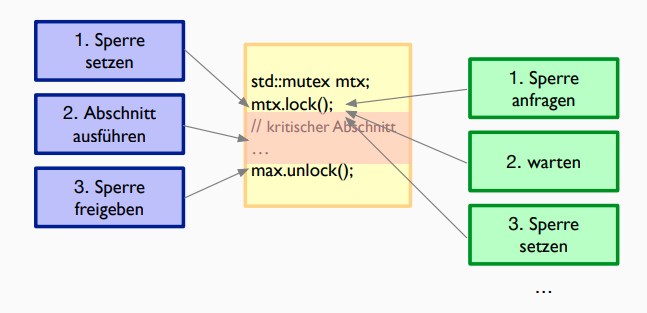
\includegraphics[width=0.4\linewidth]{Assets/Programmierparadigmen-mutex-c}
  \end{center}
  
  \paragraph{Mutex-Varianten}
  
  \begin{itemize*}
    \item mutex: Standard-Mutex für exklusiven Zugriff
    \item timed\_mutex: Mutex mit Timeout für Warten (try\_lock\_for())
    \item recursive\_mutex:rekursives Mutex - erlaubt mehrfaches Sperren durch einen Thread, z.B. für rekursive Aufrufe
    \item recursive\_timed\_mutex: rekursives Mutex mit Timeout
    \item shared\_mutex: Mutex, das gemeinsamen Zugriff (lock\_shared()) mehrerer Threads oder exklusiven Zugriff (lock()) ermöglicht
    \item shared\_timed\_mutex: Mutex mit Timeout und gemeinsamen Zugriff
  \end{itemize*}
  
  \paragraph{Lock Guards}
  
  \begin{itemize*}
    \item Vereinfachung der Nutzung von Mutexen durch RAII ('Ressourcenbelegung ist Initialisierung')
    \item Konstruktor = lock
    \item Destruktor = unlock
  \end{itemize*}
  
  \begin{lstlisting}[language=C++]
    std::vector<int> data;
    std::mutex my_mtx;
  
    void add(int val) {
      std::lock_guard<std::mutex> guard(my_mtx);
      data.push_back(val);
    }
  
    int get() {
      std::lock_guard<std::mutex> guard(my_mtx);
      return data.front();
    }
    \end{lstlisting}
  
  \paragraph{Lock Gurads und Locks}
  
  \begin{itemize*}
    \item std::unique\_lock erweiterte Variante von lock\_guards, vermeidet aber sofortiges Sperren
    \item std::lock erlaubt gleichzeitiges deadlock-freies Sperren von 2 Mutexen
    \item Sperrstrategien: u.a.
    \begin{itemize*}
      \item std::try\_to\_lock versucht Sperre ohne Blockierung zu setzen
      \item std::adopt\_lock versucht nicht, ein zweites Mal zu sperren, wenn bereits durch den aktuellen Thread gesperrt
    \end{itemize*}
  \end{itemize*}
  
  \paragraph{Atomare Datentypen}
  
  \begin{itemize*}
    \item std::atomic\_flag = sperrfreier, atomarer Datentyp:
    \begin{itemize*}
      \item clear() setzt den Wert auf false
      \item test\_and\_set() setzt den Wert atomar auf true und liefert den vorherigen Wert
    \end{itemize*}
    \item std::atomic<bool> = mächtigere Variante, erlaubt explizites Setzen
    \begin{itemize*}
      \item operator= atomare Wertzuweisung
      \item load() liefert den aktuellen Wert
      \item read-modify-write-Operation (siehe später)
    \end{itemize*}
    \item std::atomic<T> = generische Variante für weitere Datentypen
  \end{itemize*}
  
  
  \paragraph{Synchronisation über atomare Variable}
  
  \begin{lstlisting}[language=C++]
std::list<std::string> shared_space;
std::atomic<bool> ready{false};

void consume() {
  while (!ready.load())
    std::this_thread::sleep_for(std::chrono::milliseconds(10));
  std::cout << shared_space.front() << std::endl;
  shared_space.pop_front();
}

void produce() {
  shared_space.push_back("Hallo!");
  ready = true;
}

std::thread t1(consumer);
std::thread t2(producer);
...
\end{lstlisting}
  Erläuterungen
  \begin{itemize*}
    \item Zeile 1: gemeinsam genutzte Liste - erfordert synchronisierten Zugriff
    \item Zeile 2: atomare boolsche Variable ready
    \item Zeile 4/12: Konsument/Produzent-Threads
    \item Zeile 5: atomares prüfen der ready-Variablen
    \item Zeile 6-7 kurz warten und neu versuchen
    \item Zeile 8-9/13 Zugriff auf gemeinsame Liste
    \item Zeile 14: atomares Setzen der Variablen ready
  \end{itemize*}
  
  \subsubsection{Taskparallelität: Die 5 speisenden Philosophen}
  \begin{itemize*}
    \item fünf Philosophen teilen sich eine Schüssel Sphagetti
    \item fünf Gabeln, je eine zwischen zwei Philosophen
    \item Philosoph kann nur mit zwei benachbarten Gabeln essen
    \item Gabeln werden nur nach dem Essen zurückgelegt
    \item Philosoph durchläuft Zyklus von Zuständen: denken $\rightarrow$ hungrig $\rightarrow$ essen $\rightarrow$ denken $\rightarrow$ etc.
  \end{itemize*}
  
  \paragraph{Das Problem mit den Philosophen}
  
  \begin{itemize*}
    \item Jeder greift die linke Gabel
    \item und wartet auf die rechte Gabel
    \item ... und wartet ...
  \end{itemize*}
  \begin{center}
    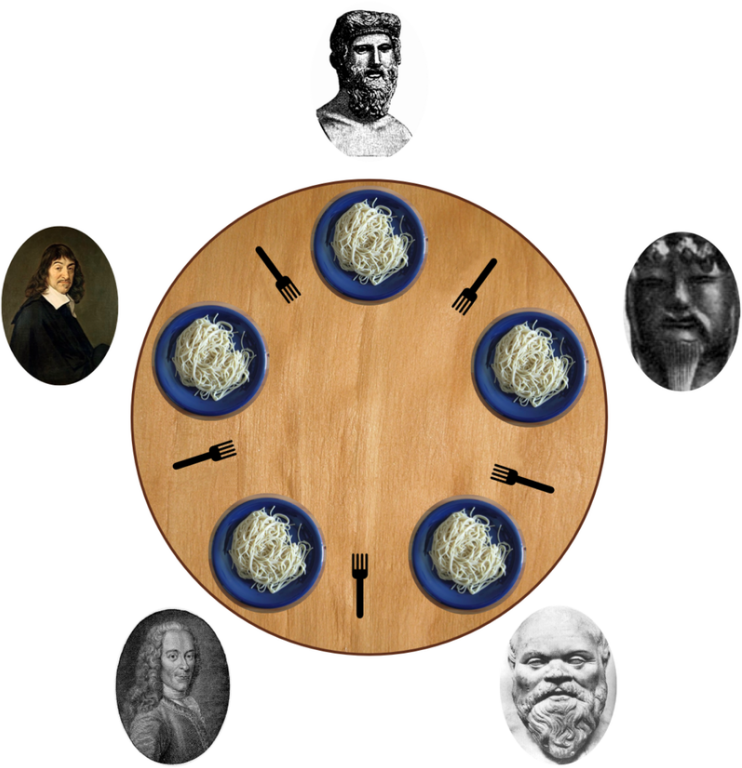
\includegraphics[width=0.3\linewidth]{Assets/Programmierparadigmen-philosophen}
  \end{center}
  \color{orange} \textbf{Verklemmung!} \color{black}
  
  \paragraph{Lösungsidee}
  
  \begin{itemize*}
    \item immer beide Gabeln aufnehmen, dh. wenn nur eine Gabel verfügbar ist: liegen lassen und warten
    \item synchronisierter Zugriff auf Gablen, dh. in einem kritischen Abschnitt unter gegenseitige Ausschluss
    \item Wecken von wartenden Philosophen
  \end{itemize*}
  
  \paragraph{Verklemmungsfreies Sperren}
  
  \begin{lstlisting}[language=C++]
  std::lock(mtx1, mtx2);
  std::lock_guard<std::mutex> lk1(mtx1, std::adopt_lock);
  std::lock_guard<std::mutex> lk2(mtx2, std::adopt_lock);
  \end{lstlisting}
  Führt zu Verklemmung; Alternative Lösung
  \begin{lstlisting}[language=C++]
  std::unique_lock<std::mutex> lk1(mtx1, std::defer_lock);
  std::unique_lock<std::mutex> lk2(mtx2, std::defer_lock);
  std::lock(lk1, lk2);
  \end{lstlisting}
  
  \paragraph{Gabeln und Spaghetti-Teller}
  \begin{lstlisting}[language=C++]
// Gabel = Mutex
struct fork {
  std::mutex mtx;
};

// 1 Teller mit 5 Gabeln
struct spaghetti_plate {
  // Benachrichtigung der Philosophen
  std::atomic<bool> ready{false}
  std::array<fork, 5> forks;
}
\end{lstlisting}
  
  \paragraph{Die Philosophen-Klasse}
  \begin{lstlisting}[language=C++]
class philosopher {
  private:
    int id;
    spaghetti_plate& plate;
    fork& left_fork;
    fork& right_fork;
  public:
    philosopher(int n, spaghetti:plate& p):
      id(n), plate(p), 
      left_fork(p.forks[n]), // 1. Gabel
      right_fork(p.forks[(n+1)%5]) // 2. Gabel
      {}
    ... 
}
\end{lstlisting}
  
  \paragraph{Die Philosophen-Klasse: Hilfsmethoden}
  
  Textausgabe erfordert synchronisierten Zugriff auf cout über globalen Mutex
  \begin{lstlisting}[language=C++]
void say(const std::string& txt) {
  std::lock_guard<std::mutex> lock(out_mtx);
  std::cout << "Philosopher #" << id << txt << std::endl;
}
\end{lstlisting}
  
  Hilfsmethode für zufällige Wartezeit in Millisekunden
  \begin{lstlisting}[language=C++]
std::chrono::milliseconds wait() {
  return std::chrono::milliseconds(rand() % 500 + 100);
}
\end{lstlisting}
  
  \paragraph{Die Philosophen-Klasse: Essen}
  \begin{lstlisting}[language=C++]
void eating(){
  //Versuche, die Gabeln (verklemmungsfrei) aufzunehmen
  std::lock(left_fork.mtx, right_fork.mtx);
  std::lock_guard<std::mutex>
    left_lock(left_fork.mtx, std::adopt_lock);
  std::lock_guard<std::mutex>
    right_lock(right_fork.mtx, std::adopt_lock);
  
  // Essen simulieren
  say(" started eating.");
  std::this_thread::sleep_for(wait());
  say(" finished eating.");
}
\end{lstlisting}
  
  \paragraph{Die Philosophen-Klasse: Denken}
  \begin{lstlisting}[language=C++]
void thinking() {
  say(" is thinking.");
  // Wenn Philosophen denken ...
  std::this_thread::sleep_for(wait());
}
\end{lstlisting}
  
  \paragraph{Das Leben eines Philosophen}
  
  \begin{itemize*}
    \item Zur Erinnerung: überladener ()-Operator eines Objekts definiert auszuführende Funktion eines Threads
  \end{itemize*}
  \begin{lstlisting}[language=C++]
void operator()(){
  // Warten bis der Teller bereit ist
  while(!plate.ready);
  do{
    //solange der Teller bereit ist
    thinking();
    eating();
  } while (plate.ready);
}
\end{lstlisting}
  
  \paragraph{Das Dinner: Initialisierung}
  \begin{lstlisting}[language=C++]
// der Teller
spaghetti_plate plate;

// die 5 Philosophen
std::array<philosopher, 5> philosophers {{
  {0, plate}, {1, plate},
  {2, plate}, {3, plate},
  {4, plate}
}};

// Thread pro Philosoph erzeugen
std::array<std::thread, 5> threads;
for (auto i=0u; i<threads.size(); i++){
  threads[i] = std::thread(philosophers[i]);
}
\end{lstlisting}
  
  \paragraph{Das Dinner beginnt}
  
  \begin{itemize*}
    \item Beginn (und Ende) des Dinners über atomare Variable signalisieren
    \item Philosophen-Threads arbeiten ihre operator()()-Methode ab
  \end{itemize*}
  \begin{lstlisting}[language=C++]
// das Essen beginnt und dauert 5 Sekunden
std::cout << "Starting dinner ..." << std::endl;
plate.ready = true;
std::this_thread::sleep_for(std::chrono::seconds(5));
// Abräumen
plate.ready = false;
// Warten auf Beendigung der Threads
std::for_each(threads.begin(), threads.end(), std::mem_fn(&std::thread::join));
std::cout << "Dinner finished" << std::endl;
\end{lstlisting}
  
  \paragraph{Fazit}
  
  \begin{itemize*}
    \item Philosophenproblem: klassisches Problem der Informatik zur Demonstration von Nebenläufigkeit und Verklemmung
    \item von Edsger W. Dijkstra formuliert
    \item betrachte C++ Lösung illustriert
    \begin{itemize*}
      \item Nebenläufigkeit durch Threads
      \item Synchronisation über Mutexe
      \item verklemmungsfreies Sperren
    \end{itemize*}
    \item moderene C++ Sprachversion vereinfacht Programmierung gegenüber Low-Level-API auf Betriebssystemebene (z.B. pthreads)
  \end{itemize*}
  
  \subsubsection{Weitere Möglichkeiten der Thread-Interaktion}
  \begin{itemize*}
    \item bisher:
    \begin{itemize*}
      \item Mutexe und Locks
      \item atomare Variablen
    \end{itemize*}
    \item typischer Anwendungsfall: Warten auf Ereignis / Setzen eines Flags
  \end{itemize*}
  \begin{lstlisting}[language=C++]
bool ready;
std::mutex mtx;

//Warten ...
std::unique_lock<std::mutex> l(mtx);
while(!flag){
  l.unlock();
  std::this_thread::sleep_for(std::chrono::milliseconds(200));
  l.lock();
}
\end{lstlisting}
  
  \subsubsection{Bedingungsvariablen}
  \begin{itemize*}
    \item Thread wartet, bis Bedingung erfüllt ist
    \item Erfüllung der Bedingung wird durch anderen Thread angezeigt (notify) $\rightarrowtail$ 'Aufwecken' des wartenden Threads
    \item notwendig: synchronisierter Zugriff über Mutex
  \end{itemize*}
  \begin{lstlisting}[language=C++]
std::list<std::string> shared_space;
std::mutex mtx;
std::condition_variable cond;

void consume(){
  while(true){
    std::unique_lock<std::mutex> l(mtx);
    cond.wait(l, [&] {
      return !shared_space.empty();
    });
    auto data = shared_space.front();
    shared_space.pop_front();
    l.unlock();
    // data verarbeiten
  }
}
\end{lstlisting}
  
  \subsubsection{Thread-sichere Datenstrukturen}
  \begin{lstlisting}[language=C++]
void produce() {
  // data erzeugen
  std::lock_guard lg(mtx);
  shared_space.push_back(data);
  cond.notify_one();
}
\end{lstlisting}
  \begin{itemize*}
    \item Thread-Sicherheit := eine Komponente kann gleichzeitig von verschiedenen Programmbereichen (Threads) mehrfach ausgeführt werden, ohne dass diese sich gegenseitig behindern
    \item verschiedene Varianten:
    \begin{itemize*}
      \item Standard-Datenstruktur + über Mutexe/Sperren synchronisierte Zugriffe
      \item Integration der Sperren in die Datenstruktur
      \item Sperr-freie Datenstrukturen: nicht-blockierend, Vermeidung von Sperren, z.B. durch Compare/Exchange-Operationen
    \end{itemize*}
    \item async , future und promise
    \item std::future - Resultat einer asynchronen Berechnung, d.h. einer Berechnung die erst noch stattfindet
    \item std::async() - asynchrones Starten eines Tasks
    \begin{lstlisting}[language=C++]
    int long_calculation() { ... }
    std::future<int> result = std::async(long_calculation);
    // Fortsetzung der Berechnung ...
    result.wait();
    std::cout << result.get() << std::endl;
  \end{lstlisting}
    \item std::promise - erlaubt Wert zu setzen, wenn der aktuelle Thread beendet ist; oft in Kombination mit std::future eingesetzt
    \item future = Ergebnisobjekt, promise = Ergebnisproduzent
    \begin{itemize*}
      \item Warten auf Ende des Tasks (wait(), wait\_for())
      \item Ergebnis lesen (get())
    \end{itemize*}
  \end{itemize*}
  
  \subsubsection{Anforderungen}
  \begin{itemize*}
    \item mehrere Threads können gleichzeitig auf die Datenstruktur zugreifen
    \item kein Thread sieht (Zwischen-)Zustand, bei dem Invarianten der Datenstruktur durch einen anderen Thread (kurzzeitig) verletzt ist
    \item Vermeidung von Wettlaufsituationen
    \item Vermeidung von Verklemmungen
    \item korrekte Behandlung von Ausnahmen (Fehlern)
  \end{itemize*}
  
  \subsubsection{Thread-sichere Queue}
  \begin{lstlisting}[language=C++]
template <typename T>
class ts_queue {
  private:
    mutable std::mutex mtx;
    std::condition_variable cond;
    std::queue<T> the_queue;
  public:
    ts_queue() {}
    ...
};
\end{lstlisting}
  \begin{itemize*}
    \item Zeilen 1,2,6: Kapselung der std::queue-Klasse
    \item Zeile 4: Mutex für exklusiven Zugriff
    \item Zeile 5: Bedingungsvariable für Warten
  \end{itemize*}
  
  \paragraph{Thread-sichere Queue: Methode push}
  \begin{lstlisting}[language=C++]
void push(T val){
  std::lock_guard<std::mutex> l(mtx);
  the_queue.push(std::move(val));
  cond.notify_one();
}
\end{lstlisting}
  \begin{itemize*}
    \item Zeile 2: Lock Guard sichert exklusiven Zugriff
    \item Zeile 3: Element an die Queue anhängen
    \item Zeile 4: Aufwecken von eventuell wartenden Threads
  \end{itemize*}
  
  \paragraph{Thread-sichere Queue: Methode waiting\_pop}
  \begin{lstlisting}[language=C++]
void waiting_pop(T& val){
  std::lock_guard<std::mutex> l(mtx);
  cond.wait(l, [this] {return !the_queue.empty(); });
  val = std::move(the_queue.front());
  the_queue.pop();
}
\end{lstlisting}
  \begin{itemize*}
    \item Zeile 2: Lock Guard sichert exklusiven Zugriff
    \item Zeile 3: Warten bis Queue nicht mehr leer ist
    \item Zeilen 4,5: erstes Element aus der Queue entnehmen
  \end{itemize*}
  
  \subsubsection{async, future und promise}
  \begin{itemize*}
    \item std::future - Resultat einer asynchronen Berechnung, d.h. einer Berechnung die erst noch stattfindet
    \item std::async() - asynchrones Starten eines Tasks
    \begin{lstlisting}[language=C++]
  int long_calculation() {...}
  std::future<int> result = std::async(long_calculation);
  //Fortsetzung der Berechnung ...
  result.wait();
  std::cout << result.get() << std::endl;
  \end{lstlisting}
    \item std::promise - erlaubt Wert zu setzen, wenn der aktuelle Thread beendet ist, of in Kombination mit std::future eingesetzt
    \item future = Ergbenisobjekt, promise = Ergebnisproduzent
  \end{itemize*}
  
  \paragraph{Future}
  
  \begin{itemize*}
    \item Methoden zum
    \begin{itemize*}
      \item Warten auf das Ende des Tasks (wait(), wait\_for())
      \item Ergebnis lesen (get())
    \end{itemize*}
  \end{itemize*}
  \begin{center}
    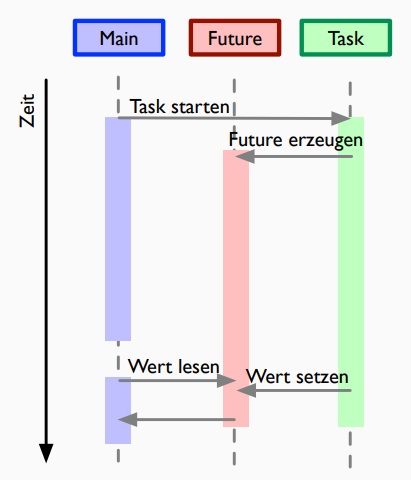
\includegraphics[width=0.4\linewidth]{Assets/Programmierparadigmen-future-task}
  \end{center}
  
  Beispiel
  \begin{lstlisting}[language=C++]
// Promise für einen String Wert
std::promise<std::string> promise;
//zugehöriges Future Objekt
auto res = promise.get_future();

//Produtenten Thread
auto producer = std::thread([&]{
  promise.set_value("Hello World");
});
//Konsumenten Thread
auto consumer = std::thread([&]{
  std::cout << res.get() << "\n";
});
producer.join();
consumer.join();
\end{lstlisting}
  
  \subsubsection{Deklarative Parallelisierung mit OpenMP}
  \begin{itemize*}
    \item Programmierschnittstelle für Parallelisierung in C/C++/Fortran
    \item Programmiersprachenerweiterung durch Direktiven
    \item in C/C++: \#pragma omp ...
    \item zusätzliche Bibliotheksfunktionen: \#include <omp.h>
    \item aktuelle Version 5.0
    \item Unterstützung in gcc und clang
    \begin{itemize*}
      \item vollständig 4.5, partiell 5.0
      \item Nutzung über Compilerflag - fopenmp
    \end{itemize*}
    \item beschränkt auf Architekturen mit gemeinsamen Speicher
  \end{itemize*}
  
  \subsubsection{Programmiermodell}
  \begin{itemize*}
    \item Master-Thread und mehrere Worker-Threads (Anzahl typischerweise durch OpenMP-Laufzeitsystem bestimmt)
    \item über parallel-Direktive kann Arbeit in einem Programmabschnitt auf Worker-Threads aufgeteilt werden
    \item Ende des parallelen Abschnitts $\rightarrowtail$ implizite Synchronisation
    \item Fortsetzung des Master-Threads
  \end{itemize*}
  \begin{center}
    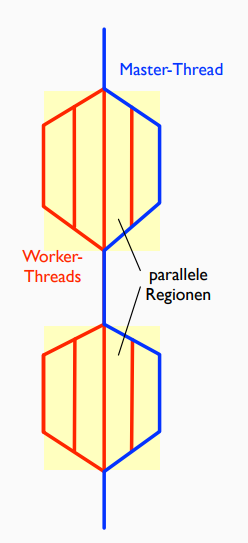
\includegraphics[width=0.2\linewidth]{Assets/Programmierparadigmen-master-worker-thread}
  \end{center}
  
  \begin{itemize*}
    \item Master-Thread und mehrere Worker-Threads (Anzahl typischerweise durch OpenMP-Laufzeitsystem bestimmt)
    \item über parallel -Direktive kann Arbeit in einem Programmabschnitt auf Worker-Threads aufgeteilt werden
    \item Ende des parallelen Abschnitts $\rightarrow$ implizite Synchronisation $\rightarrow$ Fortsetzung des Master-Threads
    \item der dem 'pragma' folgende Block wird parallel von allen Threads ausgeführt
    \begin{lstlisting}[language=C++]
    #include <iostream>
    #include <omp.h>
    int main() {
        #pragma omp parallel
        {
            std::cout << "Hello World from thread #"
            << omp_get_thread_num() << " of "
            << omp_get_num_threads() << "\n";
        }
        std::cout << "Finished!\n";
        return 0;
    }
    \end{lstlisting}
    \item Schleifenparallelisierung: jedem Thread wird ein Teil der Iteration zugewiesen (beeinflusst nur äußere Schleife)
    \begin{lstlisting}[language=C++]
  ...
  #pragma omp parallel for
    for (int i = 0; i < 20; i++) {...
  \end{lstlisting}
    \begin{itemize*}
      \item collapse(n) gibt an, dass n Schleifen in einem gemeinsamen Iterationsbereich zusammengefasst und auf die Threads verteilt werden sollen
      \begin{lstlisting}
    #pragma omp parallel for collapse(3)
    \end{lstlisting}
    \end{itemize*}
    \item Beeinflussung der Thread Anzahl
    \begin{itemize*}
      \item maximale Anzahl:
      \begin{lstlisting}
    #pragma omp parallel for num_threads(8)
    \end{lstlisting}
      \item bedingte Parallelisierung:
      \begin{lstlisting}
    #pragma omp parallel for if(i>50)
    \end{lstlisting}
    \end{itemize*}
    \item Aufteilung des Iterationsbereichs; Beeinflussung durch schedule -Direktive
    \begin{description*}
      \item[schedule(auto)] Default - implementierungsspezifisch
      \item[schedule(static, n)] statische Round-Robin-Verteilung - Bereiche der Größe n (Angabe von n ist optional)
      \item[schedule(dynamic, n)] dynamische Verteilung nach Bedarf
      \item[schedule(guided, n)] Verteilung nach Bedarf und proportional zur Restarbeit
    \end{description*}
    \item Direktiven für parallele Ausführung
    \begin{description*}
      \item[\#pragma omp single/master] Abschnitt wird nur durch einen/den Master-Thread ausgeführt
      \item[\#pragma omp critical] kritischer Abschnitt
      \item[\#pragma omp barrier] Warten auf alle Worker-Threads
      \item[\#pragma omp atomic] kritischer Abschnitt, Zugriff auf gemeinsame Variable (z.B. Zähler)
    \end{description*}
    \item Speicherklauseln für Variablen
    \begin{itemize*}
      \item 'shared' für alle Threads sichtbar/änderbar
      \item 'private' jeder Thread hat eigene Kopie der Daten, wird nicht außerhalb initialisiert
      \item 'reduction' private Daten, die am Ende des Abschnitts zu globalem Wert zusammengefasst werden
      \item 'firstprivate / lastprivate' privat - initialisiert mit letztem Wert vor dem Abschnitt / Wert des letzten Threads der Iteration wird zurückgegeben
    \end{itemize*}
    \item zuweisung von Programmabschnitten zu Threads $\rightarrow$ statische Parallelität (geeignet für rekursive Abschnitte)
    \begin{lstlisting}[language=C++]
    #pragma omp parallel sections
    {
      #pragma omp section
      qsort(data, left, p - 1);
      #pragma omp section
      qsort(data, p + 1, right);
    }
    \end{lstlisting}
    \item Task Programmierung
    \begin{itemize*}
      \item reihum Threads zugewiesen werden
      \item an beliebiger Stelle definiert werden können
      \item von beliebigem Thread definiert werden kann
    \end{itemize*}
    \begin{lstlisting}[language=C++]
    unsigned int f1, f2;
    #pragma omp task shared(f1)
      f1 = fib(f - 1);
    #pragma omp task shared(f2)
      f2 = fib(f - 2);
    #pragma omp taskwait
      return f1 + f2;
    \end{lstlisting}
  \end{itemize*}
  
  \subsubsection{Hello World! mit OpenMP}
  \begin{itemize*}
    \item der dem pragma folgende Block wird parallel von allen Threads ausgeführt
  \end{itemize*}
  \begin{lstlisting}[language=C++]
#include <iostream>
#include <omp.h>

int main() {
  #pragma omp parallel
  {
    std::cout << "Hello World from thread #"
              << omp_get_thread_num() << " of "
              << omp_get_num_threads() << "\n";
  }
  std::cout << "Finished!\n";
  return 0;
}
\end{lstlisting}
  
  \subsubsection{Schleifenparallelisierung}
  \begin{itemize*}
    \item parallele Ausführung einer Schleife: jedem Thread wird ein Teil der Iterationen zugewiesen
    \item für for-Schleifgen mit eingeschränkter Syntax (ganzzahlige Schleifenvariablen, Operatoren auf Schleifenvariablen) und für STL-Iteratoren
  \end{itemize*}
  \begin{lstlisting}[language=C++]
unsigned int results[20];
#pragma omp parallel for
for (int i = 0; i < 20; i++){
  auto f = rand() % 30;
  results[i] = fibonacci(f);
}
\end{lstlisting}
  
  \subsubsection{Beeinflussung der Thread-Anzahl}
  maximale Anzahl
  \begin{lstlisting}[language=C++]
  unsigned int results[20];
  #pragma omp parallel for num_threads(8)
  for (int i = 0; i < 20; i++){
    results[i] = fibonacci(rand() % 30);
  }
\end{lstlisting}
  
  bedingte Parallelisierung
  \begin{lstlisting}[language=C++]
  unsigned int results[20];
  #pragma omp parallel for if(i > 50)
  for (int i = 0; i < 20; i++){
    results[i] = fibonacci(rand() % 30);
  }
\end{lstlisting}
  
  \subsubsection{Aufteilung des Iterationsbereichs}
  \begin{itemize*}
    \item Iterationsbereich kann auf verschiedene Weise auf Threads aufgeteilt werden
    \item Beeinflussung durch schedule-Direktive
    \begin{description*}
      \item[schedule(auto)] Default - implementierungsspezifisch
      \item[schedule(static,n)] statische Round-Robin-Verteilung - Bereiche der Größe n (Angabe von n ist optional)
      \item[schedule(dynamic, n)] dynamische Verteilung nach Bedarf
      \item[schedule(guided, n)] Verteilung nach Bedarf und proportional zur Restarbeit
      \item[...]
    \end{description*}
  \end{itemize*}
  
  \subsubsection{Geschachtelte Schleifen}
  \begin{itemize*}
    \item Parallelisierung mit \textbf{parallel for} beeinflusst nur äußere Schleife
    \item collapse(n) gibt an, dass n Schleifen in einem gemeinsamen Iterationsbereich zusammengefasst, und auf die Threads verteilt werden sollen
    \item Beispiel: Matrizenmultiplikation
    \begin{lstlisting}[language=C++]
    #pragma omp parallel for collapse(3)
    for (int row = 0; row < m; row++)
      for(int col = 0; col < n; col++)
        for(int inner = 0; inner < k; inner++)
          prod[row][col] += A[row][inner] * B[inner][col];
  \end{lstlisting}
  \end{itemize*}
  
  \subsubsection{Synchronisation}
  \begin{itemize*}
    \item Direktiven für parallele Ausführung
    \begin{description*}
      \item[\#pragma omp single/master] Abschnitt wird nur durch einen/den Master-Thread ausgeführt
      \item[\#pragma omp critical] kritischer Abschnitt
      \item[\#pragma omp barrier] Warten auf alle Worker-Threads
      \item[\#pragma omp atomic] kritischer Abschnitt - ZUgriff auf gemeinsame Variable (z.B. Zähler)
    \end{description*}
    \item Speicherklauseln für Variablen
    \begin{description*}
      \item[shared] für alle Threads sichtbar/änderbar
      \item[private] jeder Thread hat eigene Kopie der Daten, wird nicht außerhalb initialisiert
      \item[reduction] private Daten, die am Ende des Abschnitts zu globalem Wert zusammengefasst werden
      \item[firstprivate/lastprivate] privat - initialisiert mit letztem Wert vor dem Abschnitt / Wert des letzten Threads der Iteration wird zurückgegeben
    \end{description*}
  \end{itemize*}
  
  \subsubsection{Parallele Abschnitte}
  \begin{itemize*}
    \item Zuweisung von Programmabschnitten zu Threads $\rightarrowtail$ statische Parallelität
    \item geeignet z.B. für rekursive Aufrufe
  \end{itemize*}
  \begin{lstlisting}[language=C++]
void qsort(int data[], int left, int right) {
  if( left < right) {
    int p = partition(data, left, right);
    #pragma omp parallel sections
    {
      #pragma omp section
      qsort(data, left, p -1);
      #pragma omp section
      qsort(data, p+1, right);
    }
  }
}
\end{lstlisting}
  
  \subsubsection{Task-Programmierung mit OpenMP}
  \begin{itemize*}
    \item seit OpenMP 3.0 Unterstützung von Tasks, die
    \begin{itemize*}
      \item reihum Threads zugewiesen werden
      \item an beliebiger Stelle definiert werden können
      \item von beliebigem Thread definiert werden kann
    \end{itemize*}
  \end{itemize*}
  \begin{lstlisting}[language=C++]
unsigned int fibonacci(unsigned int f){
  if( f<2 ) return n;
  unsigned int f1, f2;
  #pragma omp task shared(f1)
  f1 = fib(f-1);
  #pragma omp task shared(f2)
  f2 = fib(f-2);
  #pragma opm taskwait
  return f1 + f2;
}
\end{lstlisting}
  
  \subsubsection{Fazit}
  \begin{itemize*}
    \item C++ bietet weitreichende und mächtige Konzepte zur Parallelisierung
    \begin{itemize*}
      \item von Basiskontrolle wie Threads und Synchronisationsprimitiven (u.a. Mutexe)
      \item ...über höherwertige Abstraktionen wie async, Features und Promises
      \item bis hin zu deklarativen Ansätzen wie OpenMP
    \end{itemize*}
    \item alle Formen von Parallelität (Instruktions-, Daten-, und Taskparallelität) möglich
    \item aber anspruchsvolle Programmierung
    \item erleichtert durch zusätzliche Bibliotheken und Frameworks wie Parallel STL, TBB, ...
  \end{itemize*}
  
  \begin{lstlisting}[language=java]
//[Hello.java]
package runnable;
public class Hello {

  public class Heartbeat implements runnable {
      int pulse;
      public Heartbeat(int p) { pulse = p * 1000; }
      public void run() {
          while(true) {
              try { Thread.sleep(pulse); }
              catch(InterruptedException e) {}
              System.out.println("poch");
          }
      }
  }

  public static void main(String[] args) {
      Thread t = new Thread(new Heartbeat(2)); //Thread Objekt mit runnable erzeugen
      t.start(); //methode start() aufrufen -> ruft run() auf
  }
}
\end{lstlisting}
  \hfill
  \begin{lstlisting}[language=C++]
//[Hello.cpp]
#include <iostream> // Datei iostream aus System-Includes
#include "X.hpp" // Datei X.hpp aus Projekt-Ordner

#ifdef DEBUG // falls Konstante DEBUG definiert ist
std::cout << "Wichtige Debugausgabe" << std::endl;
#endif

#define DEBUG // Konstante setzen

class Stromfresser {
  public:
      Stromfresser() {
          std::cout << "Mjam" << std::endl;
      }
};
class Roboter : virtual public Stromfresser {};

void fun(int n, const std::string& s) {
  std::lock_guard<std::mutex> guard(my_mtx); //verklemmungsfrei mit unique_lock<std::mutex>
  for (auto i = 0; i < n; i++)
      std::cout << s << " ";
  std::cout << std::endl;
}

std::mutex my_mtx;

int main(int argc, char* argv[]){
  std::thread t(fun, 2, "Hello");
  t.join();
  return 0;
}
\end{lstlisting}
  \hfill
  \begin{lstlisting}[language=erlang]
%[Hello.erl]
-module(cheat_sheet).  % end with a period

%% Let these functions be called externally.
-export([countdown/1, countdown/0]).  % number of parameters - it matters!

%% atoms begin with a lower-case letter
%% Variables begin with an upper-case letter

%% Start defining a function with the most specific case first
countdown(0) ->  
  io:format("Zero!~n");  % function clauses end with a semicolon

%% Another clause of the same function, with a guard expression
countdown(Bogus) when Bogus < 0 ->
  io:format("Bad value: ~B~n", [Bogus]), % normal lines end with a comma
  error;  % return value (io:format returns 'ok')
  
%% Last clause matches any single parameter
countdown(Start) ->
  %% case and if statements return values!
  Type = case Start rem 2 of
      1 -> "odd";  % case and if clauses end with semicolons
      0 -> "even"  % except the last one
  end,  % end with comma, like a normal line
  io:format("~B is ~s~n", [Start, Type]), 
  countdown(Start - 1).  % When the function is all done, end with a period

%% This is a different function because it has a different number of parameters.
countdown() ->
  countdown(10).
\end{lstlisting}
  
  
  \subsection{Parallele Programmierung in Java}
  Unterstützung durch
  \begin{itemize*}
    \item Thread-Konzept
    \item eingebaute Mechanismen zur Synchronisation nebenläufiger Prozesse
    \item spezielle High-Level-Klassen im Package
    \newline \textbf{java.util.concurrent}
  \end{itemize*}
  
  \subsubsection{Threads in Java}
  \begin{itemize*}
    \item Repräsentiert durch Klasse \textbf{java.lang.Thread}
    \item Implementierung eines eigenen Kontrollflusses
    \item Eigene Klasse muss Runnable implementieren
    \begin{itemize*}
      \item Implementierung des Interface \textbf{java.lang.Runnable}
      \begin{itemize*}
        \item keine weitere Beeinflussung des Threads über zusätzliche Methoden notwendig
        \item soll von anderer Klasse als Thread abgeleitet werden
      \end{itemize*}
      \item Subklasse von \textbf{java.lang.Thread}
      \begin{itemize*}
        \item zusätzliche Methoden zur Steuerung des Ablaufs benötigt
        \item keine andere Superklasse notwendig
      \end{itemize*}
    \end{itemize*}
  \end{itemize*}
  
  \paragraph{Threads: Runnable-Schnittstelle}
  Eigene Klasse muss \textbf{Runnable} implementieren
  \begin{itemize*}
    \item Methode \textbf{public void run()} - wird beim Start des Threads aufgerufen
  \end{itemize*}
  \begin{lstlisting}[language=java]
public class Heartbeat implements Runnable {
    int pulse;
    public Heartbeat(int p) { pulse = p * 1000; }
    public void run() {
        while(true) {
            try { Thread.sleep(pulse); }
            catch(InterruptedException e) {}
            System.out.println("poch");
        }
    }
}
\end{lstlisting}
  
  \paragraph{Thread-Erzeugung}
  
  \begin{itemize*}
    \item Thread-Objekt mit Runnable-Objekt erzeugen
    \item Methode \textbf{start()} aufrufen
    \begin{itemize*}
      \item Ruft \textbf{run()} auf
    \end{itemize*}
  \end{itemize*}
  \begin{lstlisting}[language=java]
public static void main(String[] args) {
    Thread t = new Thread(new Heartbeat(2)); //Thread Objekt mit runnable erzeugen
    t.start(); //methode start() aufrufen -> ruft run() auf
}
\end{lstlisting}
  
  \paragraph{Subklasse von Thread}
  
  \begin{itemize*}
    \item Klasse muss von Thread abgeleitet werden
    \item Methode run() muss überschrieben werden
  \end{itemize*}
  \begin{lstlisting}[language=java]
public class Heartbeat2 implements Runnable {
    int pulse = 1000;
    public Heartbeat2() {}
    public void setPulse(int p){ pulse = p*1000; }

    public void run() {
      while(true) {
        try { Thread.sleep(pulse); }
        catch( InterruptedException e) {}
        System.out.println("poch");
      }
    }
}
\end{lstlisting}
  
  \begin{itemize*}
    \item Objekt der eigenen Thread-Klasse erzeugen
    \item Methode \textbf{start()} aufrufen
    \begin{itemize*}
      \item Ruft \textbf{run()} auf
    \end{itemize*}
    \begin{lstlisting}[language=java]
  public static voud main(String[] args) {
    Heartbeat2 t = new Heartbeat2(2);
    t.start();
  }
  \end{lstlisting}
    \item Spätere Beeinflussung durch andere Threads möglich
    \begin{lstlisting}[language=java]
  ...
  t.setPulse(2);
  \end{lstlisting}
  \end{itemize*}
  
  
  \paragraph{Threads: Wichtige Methoden}
  
  \begin{description*}
    \item[void start()] initiiert Ausführung des Threads durch Aufruf der Methode run
    \item[void run()] die eigentliche Arbeitsmethode
    \item[static void sleep(int millis)] hält die Ausführung des aktuellen Threads für 'millis' Millisekunden an; Keinen Einfluss auf andere Threads!
    \item[void join()] blockiert den aufrufenden Thread so lange, bis der aufgerufene Thread beendet ist
  \end{description*}
  
  \subsubsection{Parallele Berechnung von Fibonacci-Zahlen}
  \begin{lstlisting}[language=java]
public class Fibonacci implements Runnable {
  int fi;
  public Fibonacci(int f) {fi = f; }
  int fibo(int f){
    if( f<2 ) return 1;
    else return fibo(f-1) + fibo(f-2);
  }
  public void run() {
    int res = fibo(fi);
    System.out.println("Fibonacci(" + fi + ") = " + res);
  }
}
\end{lstlisting}
  
  Thread-Erzeugung und Ausführung
  \begin{lstlisting}[language=java]
public static voud main(String[] args) {
  Thread[] threads = new Thread[10];
  for(int i=0; i<10; i++){
    threads[i] = new Thread(new Fibonacci(40 + i));
    threads[i].start();
  }
}
\end{lstlisting}
  
  \subsubsection{Wechselseitiger Ausschluss in Java}
  Schlüsselwort \textbf{synchronized}
  \begin{itemize*}
    \item Implementierung von sogenannten Monitoren bzw. locks (exklusiven Sperren)
    \begin{itemize*}
      \item nur ein Thread darf den kritischen Abschnitt betreten
      \item alle anderen Threads, die darauf zugrifen wollen, müssen auf Freigabe warten
    \end{itemize*}
    \item für Methoden: \textbf{public synchronized void doSomething()}
    \begin{itemize*}
      \item nur ein Thread darf diese Methode auf einem Objekt zur gleichen Zeit ausführen
    \end{itemize*}
    \item für Anweisungen: \textbf{synchronized(anObject)\{...\}}
    \begin{itemize*}
      \item nur ein Thread darf den Block betreten
      \item Sperre wird durch das Objekt \textbf{anObject} verwaltet (jedem Java-Objekt ist eine Sperre zugeordnet)
    \end{itemize*}
  \end{itemize*}
  \begin{center}
    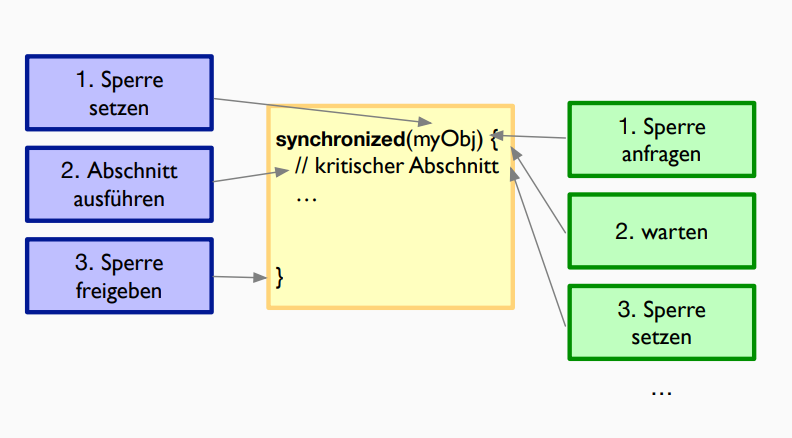
\includegraphics[width=0.4\linewidth]{Assets/Programmierparadigmen-java-synchronized}
  \end{center}
  \begin{itemize*}
    \item Schlüsselwort synchronized
    \begin{itemize*}
      \item Implementierung von sogenannten Monitoren bzw. locks (exklusiven Sperren); nur ein Thread darf den kritischen Abschnitt betreten; alle anderen Threads, die darauf zugreifen wollen, müssen auf Freigabe warten
      \item für Methoden:
      \begin{lstlisting}
      public synchronized void doSomething()
  \end{lstlisting}
      \begin{itemize*}
        \item nur ein Thread darf diese Methode auf einem Objekt zur gleichen Zeit ausführen
      \end{itemize*}
      \item für Anweisungen: synchronized(anObject) { ... }
      \begin{itemize*}
        \item nur ein Thread darf den Block betreten
        \item Sperre wird durch das Objekt anObject verwaltet (jedem Java-Objekt ist ein Sperre zugeordnet)
      \end{itemize*}
    \end{itemize*}
  \end{itemize*}
  
  \subsubsection{wait \& notify}
  \begin{description*}
    \item[] Signalisierung zwischen Threads in Java
    \item[] Basismethoden der Klasse \textbf{java.lang.Object}
    \item[wait()] der aktive Thread wartet an diesem Objekt, Sperren werden ggf. freigegeben.
    \item[notify()] wekct an diesem Objekt wartenden Thread auf
    \item[notifyAll()] weckt alle an diesem Objekt wartenden Threads auf
    \item[wait() \& notify()] dürfen nur in einem \textbf{synchronized}-Block aufgerufen werden
  \end{description*}
  
  \subsubsection{Java: High-Level-Klassen}
  \begin{itemize*}
    \item Paket \textbf{java.util.concurrent} seit Java Version 1.5
    \item Abstraktionsschicht versteckt Details über Thread-Erzeugung
    \item Übernimmt Erstellung und Überwachung von parallelen Tasks, u.a.
    \begin{description*}
      \item[ExecutorService] zum erzeugen asynchroner Tasks
      \item[Future] Referenz auf diesen Task bzw. dessen Ergebnis
      \item[ForkJoinPool \& RecursiveAction] rekursives Aufteilen eines großen Problems
    \end{description*}
  \end{itemize*}
  
  \subsubsection{Tasks und Futures in Java}
  \begin{itemize*}
    \item Task = logische Ausführungseinheit
    \item Thread = Mechanismus zur asynchronen/parallelen Ausführung von Tasks
  \end{itemize*}
  
  \begin{lstlisting}[language=java]
Runnable task = () -> {
  String me = Thread.currentThread().getName();
  System.out.println("Hallo " + me);
};
task.run();
Thread thread = new Thread(task);
thread.start();
\end{lstlisting}
  
  \subsubsection{Future \& ExecutorService}
  \begin{itemize*}
    \item \textbf{ExecutorService} stellt Methoden zum Starten/Beenden/Steuern von parallelen Aufgaben bereit
    \item implementiert \textbf{Executor}-Interface
    \begin{itemize*}
      \item definiert Methode \textbf{void execute(Runnable r)}
    \end{itemize*}
    \item Starten einer Aufgabe mit \textbf{submit}
    \begin{itemize*}
      \item \textbf{$Future<T>$ submit(Callable c)}
      \item \textbf{$Future<?>$ submit(Runnable r)}
    \end{itemize*}
    \item Zugriff auf das Ergebnis mit \textbf{get}
    \begin{itemize*}
      \item \textbf{T get(long timeout, TimeUnit unit)}
      \item \textbf{T get()}
    \end{itemize*}
  \end{itemize*}
  
  \paragraph{Future \& ExecutorService: Beispiel}
  \begin{lstlisting}[language=java]
class App {
  ExecutorService exevutor = Executors.newFixedThreadPool(4);
  void search(final String w) throws InterruptedException {
    Future<String> future = 
      executor.submit(new Callable<String>() {
        public String call(){
          return searcher.search(target);
        }
      });
    displayOtherThings(); // do other things
    try {
      displayText(future.get()); //get is blocking
    } catch (ExecutionException ex) {
      cleanup();
      return;
    }
  }
}
\end{lstlisting}
  
  \subsubsection{RecursiveAction \& Fork/Join}
  \begin{itemize*}
    \item Rekursives Zerlegen eines großen Problems in kleinere Probleme
    \item Solange bis Problem klein genug um direkt ausgeführt werden zu können
    \item Task erstellt zwei oder mehr Teiltasks von sich selbst $\rightarrowtail$ Datenparallelität
    \item ForkJoinPool zum Ausführen $\rightarrow$ implementiert Executor Interface
    \item Fazit
    \begin{itemize*}
      \item Parallelprogrammierung in Java sehr ähnlich zu C++
      \item Konzepte: Threads, kritische Abschnitte über synchronized
      \item mächtige Abstraktionen in java.util.concurrent
      \begin{itemize*}
        \item Tasks und Futures, Executor und ThreadPool
        \item thread-sichere Datenstrukturen
        \item Synchronisation: Barrieren, Semaphoren, ...
      \end{itemize*}
    \end{itemize*}
  \end{itemize*}
  
  \paragraph{Beispiel}
  \begin{lstlisting}[language=java]
class MyTask extends RecursiveAction {
  String[] source; int start, length;
  public MyTask(String[] src, int s, int l) {
    source = src; start = s; length = l;
  }

  void computeDirectly() {...}

  @Override
  void compute() {
    if(length < THRESHOLD) computeDirectly();
    else {
      int split = length / 2;
      invokeAll(new MyTask(source, start, split), new MyTask(source, start+split, length-split))
    }
  }
}
\end{lstlisting}
  
  Starten der Verarbeitung: 
  \begin{enumerate*}
    \item (große) Gesamtaufgabe erstellen
    \item ForkJoinPool erstellen
    \item Aufgabe vom Pool ausführen lassen
  \end{enumerate*}
  \begin{lstlisting}[language=java]
String[] src = ...

MyTask t = new MyTask(src, 0, src.length);
ForkJoinPool pool = new ForkJoinPool();
pool.invoke(t);
\end{lstlisting}
  
  \subsection{Zusammenfassung}
  \begin{itemize*}
    \item Parallelprogrammierung als wichtige Technik zur Nutzung moderner Hardware (Multicore, GPU, ...)
    \item verschiedene Architekturen und Programmiermodelle
    \item Instruktions-, Daten- und Taskparallelität
    \item Message Passing vs. gemeinsamer Speicher
    \item Konzepte in Erlang, C++, Java
    \item hoher Abstraktionsgrad funktionaler Sprachen
    \item C++/Java: Thread-Modell und Synchronisation mit vielen weiteren Konzepten
    \item höherwertige Abstraktion durch zusätzliche Bibliotheken und Programmierschnittstellen
  \end{itemize*}
  
  \newpage
  \section{Verteilte Programmierung}
  
  \subsection{Grundlagen}
  \subsubsection{Lernziele}
  \begin{itemize*}
    \item Verständnis von Techniken verteilter Programmierung als Paradigma
    \begin{itemize*}
      \item Modelle und Konzepte unabhängig von Programmiersprache und Betriebssystem
      \item Herausforderungen und Besonderheiten verteilter Programme
    \end{itemize*}
    \item Kennenlernen konkreter Konzepte und Mechanismen
    \begin{itemize*}
      \item praktische Beispiele in Java, Erlang und C++
      \item Bewertung und Vergleich verschiedener Plattformen
    \end{itemize*}
  \end{itemize*}
  
  \subsubsection{Einordnung}
  \begin{center}
    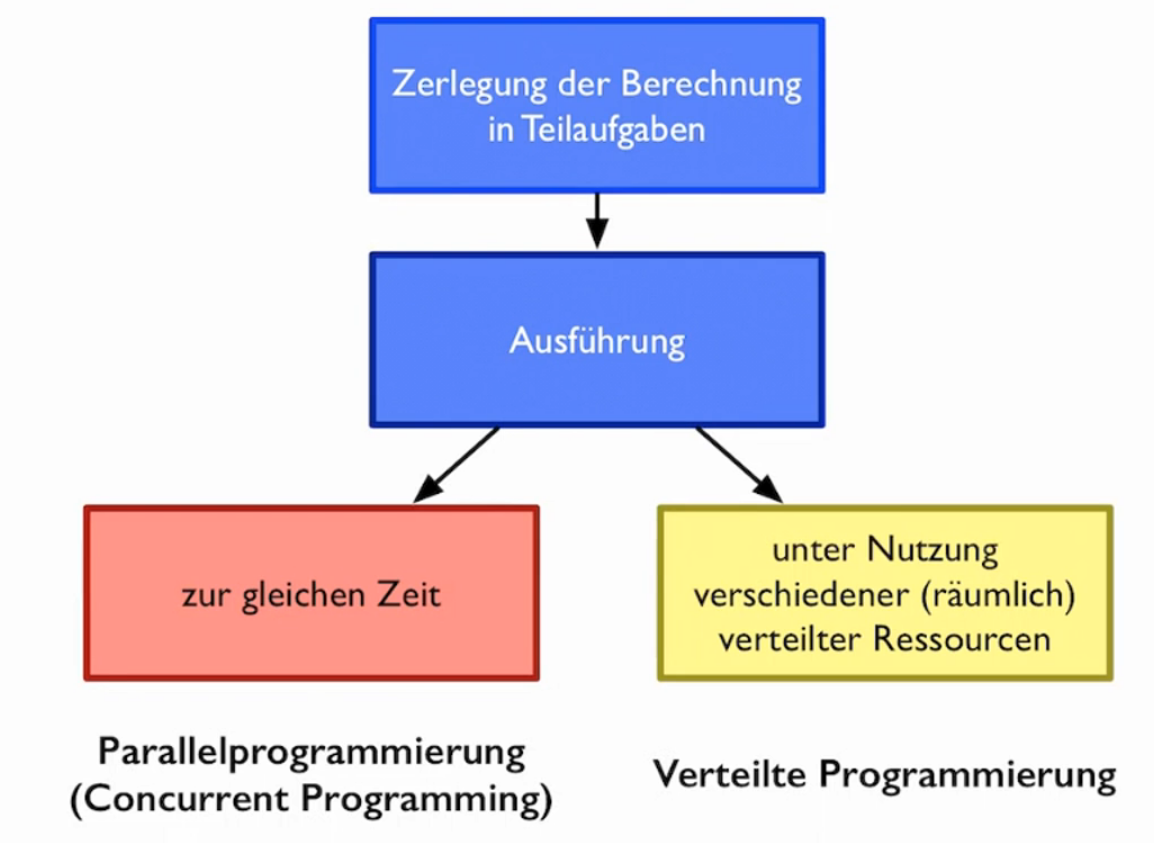
\includegraphics[width=0.4\linewidth]{Assets/Programmierparadigmen-einordnung-programmierung}
  \end{center}
  \begin{itemize*}
    \item mehrere Rechner
    \item Prozesse auf verschiedenen Rechnern
    \item Kommunikation über Knotengrenzen hinweg
    \item Behandlung von Knoten- oder Netzwerkausfällen
  \end{itemize*}
  
  \subsubsection{Ziele}
  \begin{itemize*}
    \item Bisher:
    \begin{itemize*}
      \item eine Maschine
      \item Prozesse kommunizieren nur innerhalb dieser Maschine (shared Memory vs. Message Passing)
    \end{itemize*}
    \item Jetzt:
    \begin{itemize*}
      \item mehrere Rechner
      \item Prozesse auf verschiedenen Rechnern
    \end{itemize*}
    \item Erfordert:
    \begin{itemize*}
      \item Kommunikation über Knotengrenzen hinweg
      \item Behandlung von Knoten- oder Netzwerkausfällen
    \end{itemize*}
  \end{itemize*}
  
  \subsubsection{Motivation}
  \begin{itemize*}
    \item viele verschiedene Systeme (Knoten) zur Verfügung
    \begin{itemize*}
      \item PC, Server, virtuelle Maschinen
      \item Lastverteilung, Spezialisierung auf bestimmte Probleme
    \end{itemize*}
    \item Knoten sind über Netzwerke verbunden
    \begin{itemize*}
      \item LAN(Wohnräume, Büros,...): bis zu 10 Gbit/s
      \item MAN(Metropolitan Area Network, Behördennetze, dicht besiedelte Regionen): bis zu 10 Gbit/s
      \item WAN(Wide Area Network, weltweite Vernetzung): hohe Kapazitäten zwischen den ISPs
    \end{itemize*}
  \end{itemize*}
  
  Wofür werden verteilte Systeme eingesetzt? 
  \begin{itemize*}
    \item Gemeinsame Nutzung von Ressourcen
    \begin{itemize*}
      \item Cloud-Umgebungen
      \item verteilte Datenbanksysteme
    \end{itemize*}
    \item Teilaufgaben in großen Anwendungen
    \begin{itemize*}
      \item parallele Ausführung
      \item getrennte Teilaufgaben (Micro-Services)
    \end{itemize*}
    \item Informationsaustausch
    \begin{itemize*}
      \item Email, Messenger
      \item verteilte Algorithmen
    \end{itemize*}
  \end{itemize*}
  
  \subsubsection{Software Architekturen}
  \begin{enumerate*}
    \item Früher: Hardware, Betriebssystem, Anwendung
    \begin{itemize*}
      \item Virtualisierung von Prozessor, Speicher, E/A Systemen
      \item Interprozesskommunikation (IPC)
    \end{itemize*}
    \item Middlewaresysteme: Hardware, OS, Middleware, Anwendung
    \begin{itemize*}
      \item verteilte Dienste
      \item Programmierparadigmen: RPC, Client/Server,...
      \item Java, CORBA, ...
    \end{itemize*}
    \item Heute: Virtualisierung
    \begin{itemize*}
      \item VM Hypervisor: verstecken Hardware vor dem Betriebssystem
      \item Docker: eine Anwendung pro Container
    \end{itemize*}
  \end{enumerate*}
  
  \subsubsection{Herausforderungen}
  \begin{itemize*}
    \item viele verschiedene Computer/Server
    \begin{itemize*}
      \item verschiedene Betriebssysteme
      \item unterschiedliche Leistungsfähigkeit
    \end{itemize*}
    \item Systemkomponenten müssen miteinander kommunizieren
    \item verteilte Algorithmen: Nachrichten senden, empfangen, bestätigen, Synchronisation
    \item Knotenausfälle behandeln
  \end{itemize*}
  \color{orange} $\Rightarrow$ brauchen Modelle zur Beschreibung der Kommunikation \color{black}
  
  \subsubsection{Anforderungen}
  \color{orange} Anforderungen an Kommunikationsmodelle in ... \color{black}
  \newline
  ... verteilten Systemen
  \begin{itemize*}
    \item Korrektheit
    \item Sicherheit
    \item Verfügbarkeit
    \item Skalierbarkeit
    \item Heterogenität
  \end{itemize*}
  
  ...verteilten Verkehrsmanagementsystemen
  \begin{itemize*}
    \item Echtzeitfähigkeit
    \item Offenheit
    \item Korrektheit, Sicherheit
    \item Skalierbarkeit, Verfügbarkeit
  \end{itemize*}
  
  \color{orange} Anforderungen \color{black} an den Betrieb eines (großen) verteilten Systems
  \begin{itemize*}
    \item (Last-)Skalierbarkeit (Scale-out):
    \begin{itemize*}
      \item viele kleine Server - statt eines großen
      \item neue Server nach Bedarf hinzuzufügen
    \end{itemize*}
    \item Funktionssicherheit (Safety) / IT-Sicherheit (Security)
    \item Fehlertoleranz / Verfügbarkeit
    \begin{itemize*}
      \item Ausfälle von einzelnen Knoten kompensieren
      \item Redundante Verarbeitung
    \end{itemize*}
    \item Offenheit / Interoperabilität
    \begin{itemize*}
      \item neue Knoten und Systeme einfach integrieren
    \end{itemize*}
    \item Transparenz
    \begin{itemize*}
      \item verstecke die vielen Server vor den Nutzern
    \end{itemize*}
  \end{itemize*}
  
  \subsection{Grundlagen verteilter Programmierung in Java und Erlang}
  \subsubsection{Sockets}
  \begin{itemize*}
    \item Verteilte Programmierung: Wir müssen einen entfernten Computer ansprechen
    \item benötigen: Adresse $\rightarrow$ IP-Adresse
    \item da mehrere Dienste auf demselben Computer laufen lauscht jeder Dienst auf einem Port (Nummer)
    \begin{itemize*}
      \item Wichtige Ports: 80 WWW, 20 (FTP), 25 (SMTP)
    \end{itemize*}
    \item \textbf{Socket} beschreibt einen Endpunkt, dh. Adresse und Port in einem TCP (oder UDP) Netzwerk
    \item \textbf{Server-Socket} wartet auf Verbindungen
    \item \textbf{Client} initiiert Verbindung, ebenfalls über einen (Client-Socket)
  \end{itemize*}
  
  \subsubsection{Sockets in Java}
  Socket in dem package ''java.net.Socket''
  \begin{itemize*}
    \item einen \textbf{ServerSocket} auf Port 4242 erstellen 
    \begin{lstlisting}[language=java]
      ServerSocket serverSocket = new ServerSocket(4242); 
    \end{lstlisting}
    \item Warte \color{orange}blockierend \color{black} auf Verbindungen
    \begin{lstlisting}[language=java]
      Socket client = serverSocket.accept(); 
    \end{lstlisting}
    \item Client Socket erstellen und zum Server verbinden
    \begin{lstlisting}[language=java]
      Socket client = new Socket("localhost",4242); 
    \end{lstlisting}
    \item Sockets in ähnlicher Form in C++
  \end{itemize*}
  
  \paragraph{Sockets in Java - Beispiel}
  
  Echo Server (Serverseite)
  \begin{lstlisting}[language=C++]
  ServerSocket server = new ServerSocket(4242);
  while(true){
    try(Socket client = server.accept(); ){
      Scanner in = new Scanner(client.getInputStream());
      PrintWriter out = new PrintWriter(client.getOutputStream(), true);
      String line = in.readLine();
      out.println(line);
    }
    catch ( Exception e) { e.printStackTrace(); }
  }
\end{lstlisting}
  
  Echo Server (Clientseite)
  \begin{lstlisting}[language=C++]
  try(Socket server = new Socket("localhost", 4242); ){
    Scanner in = new Scanner(client.getInputStream() );
    PrintWriter out = new PrintWriter(server.getOutputStream(), true);
    out.println("Hello World");
    System.out.println(in.nextLine());
  }
  catch ( Exception e) { e.printStackTrace(); }
  \end{lstlisting}
  
  \subsection{Aktormodell in Erlang}
  \begin{itemize*}
    \item formales Modell für Nebenläufigkeit und Verteilung
    \item Basis für verschiedene Programmiersprachen/Frameworks: Erlang, Akka (Scala/Java)
    \item Prinzipien:
    \begin{itemize*}
      \item Aktor kapselt Zustand und Verhalten
      \item Aktoren sind aktiv
      \item Aktoren kommunizieren durch Nachrichtenaustausch
      \begin{itemize*}
        \item Nichtblockierendes Senden
        \item Blockierendes Empfangen
      \end{itemize*}
    \end{itemize*}
  \end{itemize*}
  
  \subsubsection{Übersicht}
  \begin{center}
    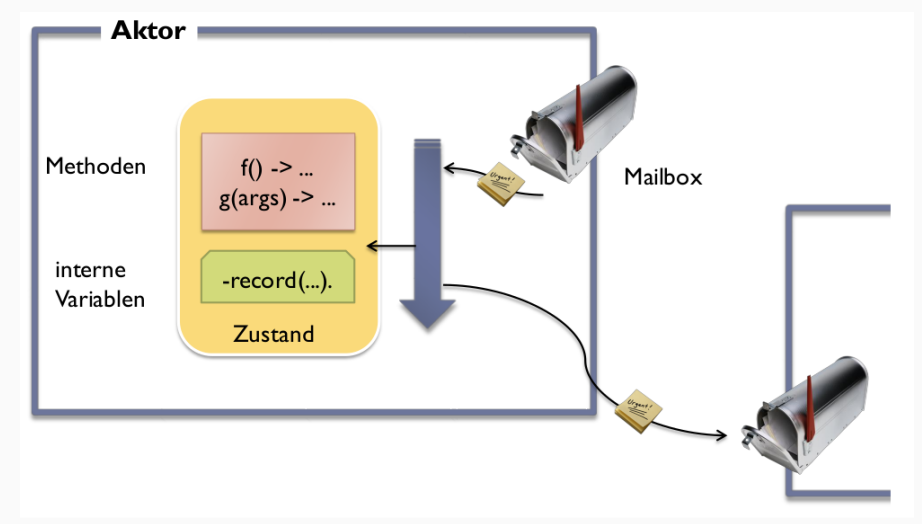
\includegraphics[width=0.4\linewidth]{Assets/Programmierparadigmen-Aktormodell.png}
  \end{center}
  
  \begin{itemize*}
    \item Aktormodell in Erlang nativ umgesetzt
    \begin{itemize*}
      \item Sende- und Empfangsoperationen schon für parallele Programmierung benutzt
      \item bisher aber nur auf einem Knoten
    \end{itemize*}
    \item Programmbestandteile im Aktormodell
    \begin{itemize*}
      \item Verhaltensdefinition $\Rightarrow$ f() $\rightarrow$ ... end.
      \item Erzeugen neuer Aktoren $\Rightarrow$ Pid = spwan(fun ...).
      \item Empfangen von Nachrichten $\Rightarrow$ receive ... end.
      \item Senden $\Rightarrow$ Pid ! Request.
    \end{itemize*}
    \item kein globaler Zustand
  \end{itemize*}
  
  \subsubsection{Kommunikation zwischen Erlangknoten}
  Erlangknoten starten (sname = short name)
  \begin{lstlisting}[language=erlang]
  #erl -sname node1 -setcookie 1234
   Eshell V11.0 (abort with ^G)
   (node1@localhost)1>
  \end{lstlisting}
  
  Weiteren Erlangknoten starten (selber oder anderer PC)
  \begin{lstlisting}[language=erlang]
  #erl -sname node2 -setcookie 1234
    Eshell V11.0 (abort with ^G)
    (node2@localhost)1>
  \end{lstlisting}
  
  Liste der verbundenen Knoten
  \begin{lstlisting}[language=erlang]
  (node@localhost)1> nodes().
  []
  \end{lstlisting}
  
  \subsubsection{Cookie-System}
  \begin{itemize*}
    \item verteilte Erlangknoten benötigen zur Kommunikation gemeinsames \color{orange} Magic Cookie \color{black} (Passwort)
    \item Mehrere Varianten
    \begin{itemize*}
      \item Datei {\raise.17ex\hbox{$\scriptstyle\mathtt{\sim}$}}/.erlang.cookie
      \item Erlang-Funktion
      \begin{lstlisting}[language=erlang]
      :set_cookie(node(), Cookie).
      \end{lstlisting}
      \item Option
      \begin{lstlisting}
      erl -setcookie Cookie
      \end{lstlisting}
    \end{itemize*}
  \end{itemize*}
  
  \subsubsection{Verbindungsaufbau zwischen Erlangknoten}
  Verbindungsaufbau mittels \color{blue} net\_adm:\color{black}ping Funktion
  
  \begin{lstlisting}[language=erlang]
  (node1@localhost)2> net_adm:ping("node2@localhost").
  pong
  (node1@localhost)3> nodes().
  ["node2@localhost"]

  (node2@localhost)1> nodes().
  ["node1@localhost"]
  \end{lstlisting}
  
  \subsubsection{Kommunikation zwischen Erlangknoten}
  Starten eines Prozesses auf einem entfernten Host
  
  \begin{lstlisting}[language=erlang]
  complicated() ->
    receive
      {Sender, I} -> Sender ! I*I
    end.

  sender(Num, Pid) ->
    Pid ! {self(), Num},
    receive
      Res -> io:format("Result = ~p~n", [Res])
  (node1@localhost)4> N2Pid = spawn("node2@localhost", fun ch5_1:complicated/0)
  (node1@localhost)5> ch5_1:sender(25, N2Pid).
  Result = 625
  ok
  \end{lstlisting}
  
  \subsection{Alternating Bit Protokoll}
  \subsubsection{Übersicht}
  \begin{itemize*}
    \item ermöglicht es, Nachrichten über einen verlustbehafteten Kommunikationskanal vollständig zu übertragen, sofern Verluste nur gelegentlich auftreten (transiente Fehler)
    \item Empfänger quittiert jedes erhaltene Paket (Achnowledgement, kurz ACK)
    \item \textbf{Achtung} Kanal kann Nachrichten und ACKs verlieren
    \begin{itemize*}
      \item benötigen je zwei unterschiedliche Sequenznummern und ACKs
    \end{itemize*}
    \item Empfänger liefert eine Nachricht nur beim ersten Empfang aus (keine Duplikate)
    \item bei Timeout: Nachricht erneut senden
    \item bei Erhalt eines unerwarteten ACKs: \textbf{aktuelle Nachricht erneut senden}
  \end{itemize*}
  
  \subsubsection{Zustände}
  \begin{center}
    \includegraphics[width=0.4\linewidth]{Assets/Programmierparadigmen-zustände-bit-protokoll}
  \end{center}
  
  \subsubsection{Das Alternating Bit Protokoll}
  Wir implementieren eine Variante, bei welcher: 
  \begin{itemize*}
    \item der Sender zu Beginn eine Liste mit sämtlichen zu sendenden Nachrichten erhält, und
    \item der Empfänger die erstmals empfangenen Nachrichten einfach auf dem Bildschirm ausgibt
    \item alle Aktoren Statusmeldungen ausgeben
    \item Verluste über einen Zufallszahlengenerator ausgelöst werden
  \end{itemize*}
  \begin{center}
    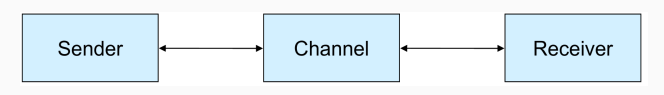
\includegraphics[width=0.4\linewidth]{Assets/Programmierparadigmen-alternate-bit-protokoll.png}
  \end{center}
  drei Prozesse mit \textbf{initialize(ErrorRate, NumberOfMessages, ReceiverPid, SenderPid, ChannelPid)} initialisieren und starten
  \begin{itemize*}
    \item Sender hat vier Zustandsfunktionen; Startet mit senderReady0(List): Liste mit Zahlen 1,...,NumberOfMessages
    \item Kanal: Nachricht 'verlieren', wenn Zufallszahl $\ngeq$ ErrorRate
    \item Empfänger hat zwei Zustandsfunktionen; zu Beginn wird receiverWait0 gestartet
    \item initialize wartet auf eine ready-Nachricht; sendet danach stop-Nachrichten an alle
  \end{itemize*}
  \begin{lstlisting}[language=erlang]
-module(altbit).
-export([initialize/5]).
-import(rand, [seed/3, uniform/0]).

for(Max, Max, F) -> [F(Max)]; % for convemience
for(I, Max, F) -> [F(I)|for(I+1, Max, F)]
\end{lstlisting}
  
  \begin{lstlisting}[language=erlang]
initialize(ErrorRate, NumberOfMessages, R, S, C) ->
  rand:seed({23, 13, 97}), %initialised RND
  SendList = for(1, NumberOfMessages, fun(I) -> I end),
  register(initializer, seld()), % others may send us 'ready'
  Receiver = spawn(R, fun() -> receiverWait0() end),
  register(receiver, Receiver),
  Channel = spawn(C, fun() -> channelIdle(ErrorRate) end),
  register(channel, Channel),
  Sender = spawn(S, fun() -> senderReady0(SendList) end),
  register(sender, Sender),
  io:format("Started ABP with ~.10B Messages and Error Rate ~f~n", [NumberOfMessages, ErrorRate]),
  receive % wait for Signal that all Messages went ok
    ready -> io:format("All ~.10B Messages sent.~n", [NumberOfMessages])
  end, % Now clean up everything
  Sender ! stop, Receiver ! stop, Channel ! stop,
  unregister(initializer)
\end{lstlisting}
  
  \begin{lstlisting}[language=erlang]
senderReady0([]) -> initializer ! ready;
senderReady0([M|MS]) ->
  channel ! {receiver, {seq0, M}},
  io:format("Sender: sends Message ~.10B. ~n",[M]),
  senderProcess0([M|MS]).
\end{lstlisting}
  
  \begin{lstlisting}[language=erlang]
senderProcess0([]) -> initializer!ready; %to be safe
senderProcess0([M|MS]) ->
  receive
    ack0 -> io:format("Sender: received expected Ack for Message ~.10B. ~n", [M]);
    ack1 -> io:format("Sender: received unexpected Ack; Send Again Message ~.10B.~n", [M]),
      channel ! {receiver, {seq0, M}},
      senderProcess0([M|MS]);
    stop -> true
    after 1000 -> io:format("Sender: Timeout! Repeat Message ~.10B. ~n", [M]),
      channel ! {receiver, {seq0, M}},
      senderProcess0([M|MS])
  end.
\end{lstlisting}
  
  \begin{lstlisting}[language=erlang]
cannelIdle(ErrorRate) ->
  RN = uniform(), % for determining if msg to be dropped
  receive
    {receiver, {Seq, M}} when RN =< ErrorRate -> %drop
      io:format("Channel: drops Message ~.10B. ~n", [M]),
      channelIdle(ErrorRate);
    {receiver, {Seq, M}} when RN > ErrorRate -> % deliver
      receiver!{Seq, M},
      channelIdle(ErrorRate);
    {sender, M} when RN =< ErrorRate -> %drop
      io:format("Channel: drops ~w ~n", [M]),
      channelIdle(ErrorRate);
    {sender, M} when RN > ErrorRate -> %deliver
      sender ! M,
      channelIdle(ErrorRate);
      stop -> true
  end.
\end{lstlisting}
  
  \begin{lstlisting}[language=erlang]
receiverWait0() ->
  receive
    {seq0, M} ->
      io:format("Receiver: received and delivers Message ~.10B. ~n",[M]),
      channel ! {sender, ack0},
      receiverWait1();
    {seq1, M} ->
      io:format("Receiver: ignores unexpected Message ~.10B. ~n", [M]),
      channel ! [sender, ack1],
      receiverWait0();
    stop -> true
  end.  
\end{lstlisting}
  
  \begin{lstlisting}[language=bash]
> altbit:initialize(0.45, 3, 'receiver@pc1', 'channel@pc2', 'sender@pc3').
Started ABP with 3 Messages and Error-Rate 0.450000
Sender: sends Message 1.
Channel: drops Message 1.
Sender: Timeout! Send Again Message 1.
Channel: drops Message 1.
Sender: Timeout! Send Again Message 1.
Receiver: received and delivers Message 1.
Sender: received expected Ack for Message 1.
Sender: sends Message 2.
Receiver: received and delivers Message 2.
Channel: drops ack1
Sender: Timeout! Send Again Message 2.
Receiver: ignores unexpected Message 2.
Sender: received expected Ack for Message 2.
Sender: sends Message 3.
Receiver: received and delivers Message 3.
Sender: received expected Ack for Message 3.
All 3 Messages successfully transmitted.
\end{lstlisting}
  
  \subsection{Kommunikationsmodelle \& Implementierungen}
  \subsubsection{Kommunikationsmodelle}
  Frage: Wie sollen Knoten miteinander kommunizieren? 
  \begin{itemize*}
    \item Sprechen die Teilnehmer direkt miteinander oder über einen Vermittler?
    \item Kann jeder jedem eine Nachricht schicken?
    \item Wartet ein Teilnehmer darauf, dass seine Nachricht angekommen ist?
    \item Wartet ein Teilnehmer darauf, dass eine Nachricht ankommt?
    \item Muss ein Teilnehmer auf eine Nachricht antworten?
  \end{itemize*}
$\Rightarrow$ das Verhalten der Teilnehmer ist in \color{orange} Kommunikationsmodellen \color{black} beschrieben
  
  \subsubsection{Arten von Kommunikationsmodellen}
  Es gibt viele verschiedene Modelle, z.B. für \color{orange} Botschaftenbasierte Modelle \color{black}
  \begin{itemize*}
    \item Auftragsorientierte Modelle
    \item Funktionsaufrufbasierte Modelle
    \item Blackboards
    \item Ereignisbasierte Modelle
    \item Strombasierte Modelle
    \item Wissensbasierte Modelle
  \end{itemize*}
  Kommunikationspartner sind für uns: 
  \begin{itemize*}
    \item Threads/Prozesse innerhalb verteilter Anwendungen
    \item Komponenten verteilter Systeme (Browser $\Leftrightarrow$ Webserver, DB Client $\Leftrightarrow$ DB-Server)
  \end{itemize*}
  
  \subsubsection{Modellbestandteile}
  \begin{itemize*}
    \item \color{orange} Rollenmodell: \color{black}
    \begin{itemize*}
      \item gemeinsames Handlungsmuster festlegen
      \item z.B. Anrufer/Angerufener, Clinet/Server, Quelle/Senke
    \end{itemize*}
    \item \color{orange} Datenmodell: \color{black}
    \begin{itemize*}
      \item einheitliche Interpretation der ausgetauschten Daten
      \item z.B. Dateiformate (XML/JSON), Kodierungen (MPEG4/H.264)
    \end{itemize*}
    \item \color{orange} Fehlersemantiken \color{black}
    \begin{itemize*}
      \item Einvernehmen über Wirkungen von Ausfällen
      \item Eigenschaften von Kommunikationsoperationen müssen bei Ausfällen garantiert werden
    \end{itemize*}
    \item \color{orange} Terminierungssemantik \color{black}
    \begin{itemize*}
      \item Einvernehmen über das Ende der Kommunikation
      \item Garantien über das Ende von Kommunikationsoperationen (auch bei Ausfällen)
    \end{itemize*}
  \end{itemize*}
  
  \subsubsection{Kommunikationsarten}
  \begin{itemize*}
    \item Wann ist eine Kommunikationsoperation abgeschlossen?
    \item entspricht Terminierungssemantik
    \item zwei grundlegende Arten:
    \begin{itemize*}
      \item \color{orange} synchron \color{black}
      \begin{itemize*}
        \item blockierend
        \item Teilnehmer wartet bis die Gegenseite bereit ist
        \item kann lange dauern, Sender kann nicht weiter arbeiten
        \item Senden: Botschaftenankunft garantiert, einfache Implementierung synchroner Aktivitäten
        \item Empfangen: Botschaftenankunft einfach und präzise feststellbar
      \end{itemize*}
      \item \color{orange} asynchron \color{black}
      \begin{itemize*}
        \item nicht-blockierend
        \item Der Teilnehmer wartet nicht auf die Gegenseite (”fire and forget”)
        \item unklar ob Botschaft angekommen
        \item Senden: einfache Implementierung von Nebenläufigkeit
        \item Empfangen: unklar wann Botschaft ankommt, einfache Implementierung von Nebenläufigkeit
      \end{itemize*}
      \item gilt sowohl für das Senden als auch das Empfangen
    \end{itemize*}
  \end{itemize*}
  
  \subsubsection{Kommunikationsarten: Senden}
  
  \color{orange} synchrones Senden: \color{black} Der Sender wartet bis der Empfänger die Botschaft annimmt
  \begin{center}
    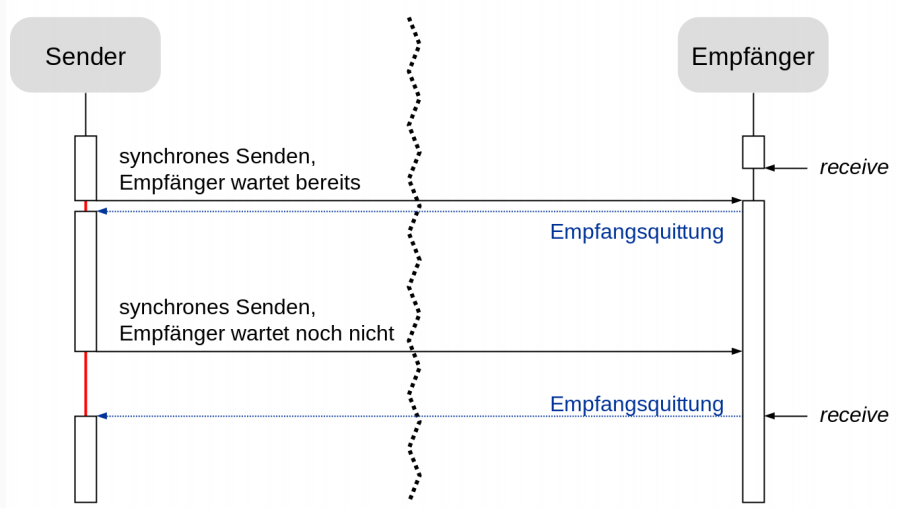
\includegraphics[width=0.4\linewidth]{Assets/Programmierparadigmen-synchrones-senden}
  \end{center}
  \noindent \color{orange} asynchrones Senden: \color{black} Der Sender wartet nicht bis der Empfänger die Botschaft annimmt ('fire and forget' Prinzip)
  \begin{center}
    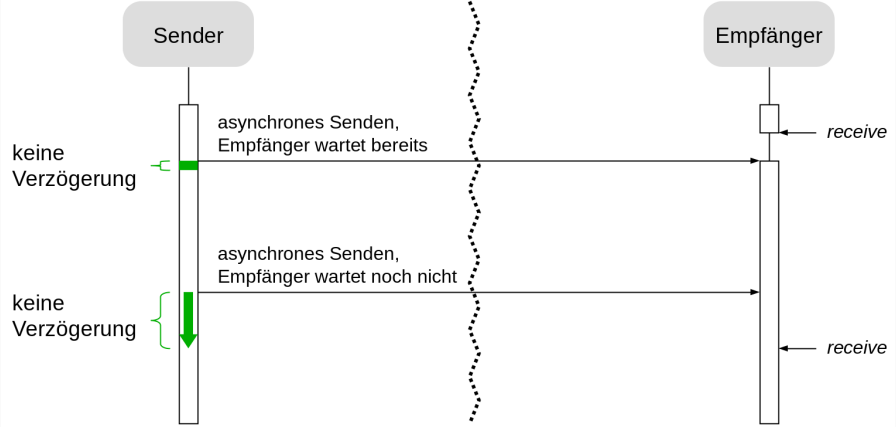
\includegraphics[width=0.4\linewidth]{Assets/Programmierparadigmen-asynchrones-senden}
  \end{center}
  
  \paragraph{Synchrones vs. asynchrones Senden}
  
  \begin{itemize*}
    \item synchrones Senden
    \begin{itemize*}
      \item kann lange dauern, der Sender kann währenddessen nicht weiterarbeiten
      \item die Botschaftenankunft ist garantiert, eine einfache Implementierung synchroner Aktivitäten
    \end{itemize*}
    \item asynchrones Senden
    \begin{itemize*}
      \item unklar ob die Botschaft angekommen ist
      \item einfache Implementierung von Nebenläufigkeit
    \end{itemize*}
  \end{itemize*}
  
  \subsubsection{Kommunikationsarten: Empfangen}
  
  \color{orange} synchrones Empfangen: \color{black} Der Empfänger wartet bis die Botschaft eintrifft
  \begin{center}
    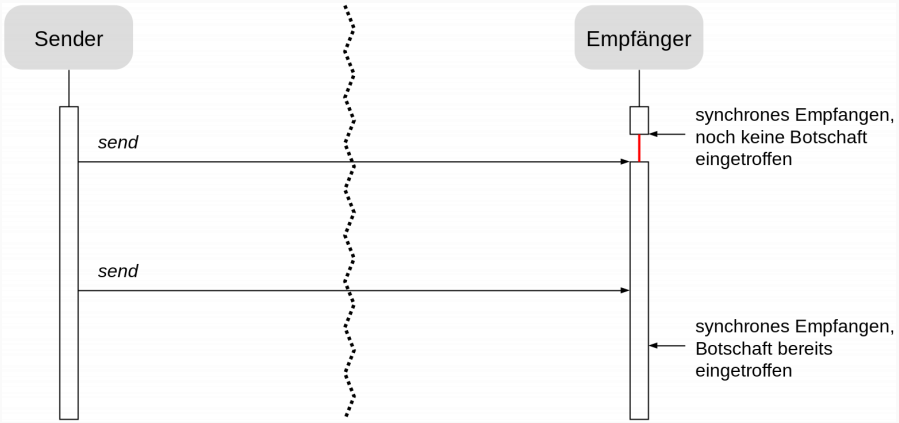
\includegraphics[width=0.4\linewidth]{Assets/Programmierparadigmen-synchron-empfangen}
  \end{center}
  \color{orange} asynchrones Empfangen: \color{black} Der Empfänger macht weiter, falls keine Nachricht eingetroffen ist
  \begin{center}
    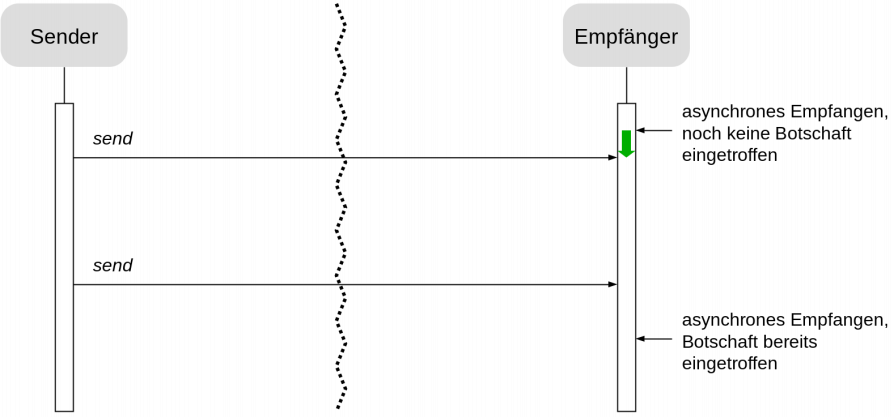
\includegraphics[width=0.4\linewidth]{Assets/Programmierparadigmen-asynchron-empfangen}
  \end{center}
  
  \paragraph{Synchrones vs. asynchrones Empfangen}
  \begin{itemize*}
    \item synchrones Empfangen:
    \begin{itemize*}
      \item kann lange dauern, der Sender kann nicht weiterarbeiten
      \item Botschaftenankunft ist einfach und präzise feststellbar
    \end{itemize*}
    \item asynchrones Empfangen:
    \begin{itemize*}
      \item unklar wann die Botschaft ankommt;
      \newline Benachrichtigungstechniken 
      \begin{itemize*}
        \item Nachfragen (Polling)
        \item ankommende Botschaft erzeugt neuen Thread beim Empfänger
        \item weitere Techniken möglich
      \end{itemize*}
      \item einfache Implementierung von Nebenläufigkeit
    \end{itemize*}
  \end{itemize*}
  
  \subsubsection{Fehlerbehandlung}
  \begin{itemize*}
    \item unverlässliches vs. verlässliches Senden
    \begin{itemize*}
      \item 'Brief vs. Einschreiben'
    \end{itemize*}
    \item verlässliche Kommunikation erfordert
    \begin{itemize*}
      \item Quittierungen (Acknowledgements) $\rightarrow$ mehr Daten senden
      \item Timeouts $\rightarrow$ Zeitverwaltung, langes Warten
    \end{itemize*}
    \item vielfältige Fehlermöglichkeiten in verteilten Anwendungen:
    \begin{itemize*}
      \item Kommunikations-/Netzwerkfehler: $\rightarrow$ Nachricht/Antwort gar nicht oder verzögert zugestellt
      \item Serverausfall: Nachricht empfangen? Operation ausgeführt?
      \item Clientausfall: Aufruf gültig? Bestätigung erhalten?
    \end{itemize*}
  \end{itemize*}
  \begin{center}
    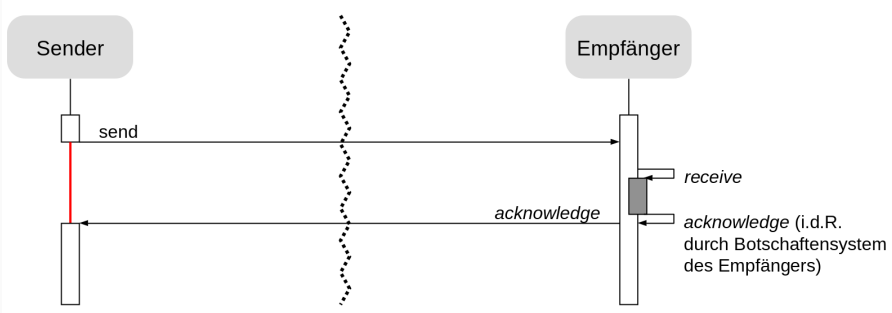
\includegraphics[width=0.4\linewidth]{Assets/Programmierparadigmen-kommunikation-fehler}
    
\includegraphics[width=0.4\linewidth]{Assets/Programmierparadigmen-kommunikation-fehler-2}
  \end{center}
  
  vielfältige Fehlermöglichkeiten in verteilten Anwendungen: 
  \begin{itemize*}
    \item Kommunikations-/Netzwerkfehler: $\rightarrow$ Nachricht/Antwort gar nicht oder nur verzögert zugestellt
    \item Serverausfall: Nachricht empfangen? Operation ausgeführt?
    \item Clientausfall: Aufruf gültig? Bestätigung erhalten?
    \item Beispiel: Reisebuchung
    \begin{itemize*}
      \item Buchung durchgeführt? Bestätigung erhalten?
      \item Bei wiederholter Ausführung: wirklich neue Buchung?
    \end{itemize*}
  \end{itemize*}
  
  \paragraph{Fehlerbehandlung in Erlang}
  
  \begin{itemize*}
    \item Timeout beim Warten auf Nachrichten
    \item Wenn keine passende Nachricht innerhalb \textbf{Time} msecs empfangen wird, dann wird der Rückgabewert des \textbf{after}-Ausdrucks verwendet.
  \end{itemize*}
  \begin{lstlisting}[language=erlang]
  receive
      {ok, Resp} -> Resp;
      {notfound} -> notfound;
      after Time -> timeout
  end
  \end{lstlisting}
  
  Umgang mit Fehlern (Timeouts, Ausfälle):
  \begin{itemize*}
    \item Maybe:
    \begin{itemize*}
      \item keine Wiederholung
      \item keine Ausführungsgarantie
    \end{itemize*}
    \item At-least-once:
    \begin{itemize*}
      \item wiederholte Ausführung, aber keine Erkennung von Nachrichtduplikaten
      \item nur für idempotente Operationen (Lesen)
    \end{itemize*}
    \item At-most-once:
    \begin{itemize*}
      \item garantiert, dass mehrfache Aufrufe nur zu einziger Ausführung führen
      \item z.B. durch Sequenznummern (erfordert Protokollierung zur Duplikateliminierung)
      \item für nicht-idempotente Operationen (schreibend, z.B. Einfügen, Löschen)
    \end{itemize*}
  \end{itemize*}
  
  \subsubsection{Überwachung von Erlang-Prozessen}
  \begin{itemize*}
    \item Linking von Prozessen: \color{green}link\color{blue}(Pid) \color{black}
    \item M überwacht S; S bricht durch Fehler ab
    \begin{center}
      \centering
      \includegraphics[width=0.4\linewidth]{Assets/Programmierparadigmen-erlang-überwachung}
    \end{center}
    \item M wartet auf EXIT Nachricht von S $\rightarrow$ asynchroner Handler nötig
  \end{itemize*}
  
  \subsubsection{on\_exit-Handler}
  \begin{lstlisting}[language=erlang]
on_exit(Pid, Fun) ->
  spawn(fun() ->
    process_flag(trap_exit, true),
    link(Pid),
    receive
      {"EXIT", Pid, Why } -> Fun(Why)
    end
  end).
\end{lstlisting}
  
  \begin{itemize*}
    \item überwacht den Prozess \textbf{Pid} auf Abbruch
    \item Anwendungsspezifische Reaktionen möglich
    \begin{itemize*}
      \item Fehlermeldung
      \item Neustart des Prozesses
    \end{itemize*}
    \item auch über Erlang-Knotengrenzen hinweg!
  \end{itemize*}
  
  \paragraph{Anwendung des on\_exit-Handlers}
  \begin{lstlisting}[language=erlang]
F = fun() -> receive X -> list_to_atom(X) end end.
Pid = spawn(F).
on_exit(Pid, fun(Why) -> io:format("~p died with ~p~n", [Pid, Why]) end).
Pid ! ping.
\end{lstlisting}
  
  \begin{itemize*}
    \item Funktion anlegen (Liste in Atom konvertieren)
    \item Prozess erzeugen
    \item \textbf{on\_exit}-Handler definieren
    \item Fehler verursachen (Nachricht ist keine Liste)
  \end{itemize*}
  
  \subsubsection{Fehlersemantiken}
  Umgang mit Fehlern (Timeouts, Ausfälle)
  \begin{itemize*}
    \item \color{orange} Maybe: \color{black}
    \begin{itemize*}
      \item keine Wiederholung
      \item keine Ausführungsgarantie
    \end{itemize*}
    \item \color{orange} At-least-once: \color{black}
    \begin{itemize*}
      \item wiederholte Ausführung, aber keine Erkennung von Nachrichtenduplikaten
      \item nur für idempotente Optionen (Lesen)
    \end{itemize*}
    \item \color{orange} At-most-once: \color{black}
    \begin{itemize*}
      \item garantiert, dass mehrfache Aufrufe nur zu einziger Ausführung führen
      \item z.B. durch Sequenznummern (erfordert Protokollierung zur Duplikatelliminierung)
      \item für nicht-idempotente Operationen (schreibend, z.B. Einfügen, Löschen)
    \end{itemize*}
  \end{itemize*}
  
  \subsubsection{Auftragsorientierte Modelle}
  \begin{itemize*}
    \item klassische Modell serviceorientierten Systemdesigns
    \item in verteilten Systemen:
    \begin{itemize*}
      \item Menge von Dienstanbietern (Server)
      \item Menge von Clients, die diese Dienste nutzen wollen
    \end{itemize*}
  \end{itemize*}
  Typische Anwendungsszenarien
  \begin{description*}
    \item[DB-Server] verwalten Datenbestände, verarbeiten SQL Anfragen
    \begin{itemize*}
      \item Clients: 'Gib mir alle Personen, die älter als 18 Jahre alt sind'
    \end{itemize*}
    \item[Web] Webserver stellt HTML Dokumente bereit, Browser ruft URLs für Dokumente auf
    \item[E-Mail] Mailserver verwalten Postfächer, leiten Mails weiter, Outlook/Thunderbird/...senden/lesen von Emails
    \item[Namensdienste (DNS), Fileserver, Zeitserver (NTP)]
  \end{description*}
  
  \paragraph{Auftragsorientierte Modelle: Modellsicht}
  
  \begin{itemize*}
    \item Rollenmodell: Clients erteilen Aufträge an Server
    \item Datenmodell: Notschaften mit vereinbarter Struktur (Protokoll)
  \end{itemize*}
  \begin{lstlisting}
POST /axis2/services/TimeWS HTTP/1.1
Content-Type: application/soap+xml; charset=UTF-8;
action="urn:getTimeOfDay"

<?xml version='1.0' encoding='UTF-8'?>
<soapenv:Envelope xmlns:soapenv="...">
  <soapenv:Body/>
</soapenv:Envelope>
\end{lstlisting}
  
  \begin{itemize*}
    \item Fehlersemantiken: Was ist der Grund, wenn ich keine Antwort erhalte?
    \begin{itemize*}
      \item Auftrag angekommen? Vollständig bearbeitet?
      \item Was passiert wenn ein Auftrag wiederholt wird?
    \end{itemize*}
    \item Terminierungssemantiken:
    \begin{itemize*}
      \item Auftragserteilung in der Regel synchron
      \item es existieren aber auch asynchrone Aufträge
    \end{itemize*}
  \end{itemize*}
  
  \paragraph{Auftragsorientierte Modelle: Implementierung}
  
  \begin{itemize*}
    \item Implementierung aufbauend auf send/receive
  \end{itemize*}
  \begin{center}
    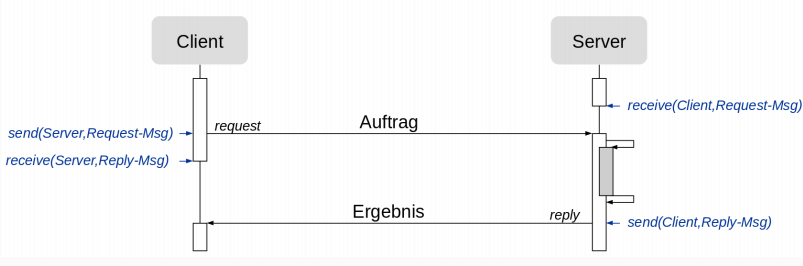
\includegraphics[width=0.4\linewidth]{Assets/Programmierparadigmen-kommunikation}
  \end{center} \ \linebreak
  
  \paragraph{Ein Fileserver in Java}
  
  Server
  \begin{lstlisting}[language=java]
try(ServerSocker ss = new ServerSocket(4242)){
  Socket s = ss.accept(); //warte auf Clients
  // ...

  String line = null;
  if((line = socketReader.readLine()) != null) {
    String command = lines.split(" "); //trenne beim Leerzeichen
    String operation = command[0]; String path = command[1];
    switch(operation.trim().toUpperCase()) {
      case "GET":
        String content = readFile(path);
        socketWriter.write(content); break;
      case "DELETE":
        boolean ok = deleteFile(path);
        socketWriter.write(String.valueOf(ok)); break;
      // ...
    } /*switch*/ } /*if*/ } /*try*/
\end{lstlisting}
  Erläuterungen zum Server
  \begin{itemize*}
    \item Zeile 1 \& 2: Serversocket erstellen, lauscht auf Port 4242, wartet blockierend bis sich ein Client verbindet
    \item Zeile 6: lies eine Zeile vom Client
    \item Zeile 7: unser Nachrichtenformat: \textbf{Operation $<$Leerzeichen$>$ Dateipfad}
    \item Zeile 8ff: unterscheide Operationen und führe Aktionen aus; antworte dem Client entsprechend
  \end{itemize*}
  
  Client
  \begin{lstlisting}[language=java]
try(Socket socket = new Socker("localhost", 4242)){
  String command = args[0] + " " + args[1];

  socketWriter.write(command);

  String response;
  while((response = socketReader.readLine()) != null) {
    System.out.println(response);
  }
}
\end{lstlisting}
  \begin{itemize*}
    \item Zeile 1: erstelle Clientsocket, d.h. Verbindungsaufbau zum Server auf localhost auf Port 4242
    \item Zeile 2: lese Befehl und Dateipfad
    \item Zeile 4: sende Befehl als String an den Server
    \item Zeile 6ff: lese alle Antwortzeilen vom Server; Ausgabe auf dem Bildschirm
  \end{itemize*}
  
  \paragraph{Auftragsorientierte Modelle}
  
  \begin{itemize*}
    \item Können benutzt werden, um einfache Protokolle zu implementieren
    \item Binär oder ASCII
    \begin{itemize*}
      \item auch Übertragung komplexer Objekte möglich
    \end{itemize*}
    \item gesendeter Befehl könnte einer Methode/Funktion auf dem Server entsprechen
    \begin{itemize*}
      \item es erfolgt eine Art entfernter Funktionsaufruf
      \item RPC wird im nächsten Abschnitt behandelt
    \end{itemize*}
    \item Funktionalität kann über das Internet angeboten werden
    \begin{itemize*}
      \item[$\Rightarrow$] Implementierung eines Webservices
    \end{itemize*}
  \end{itemize*}
  
  \subsubsection{Webservices - Allgemein}
  \begin{itemize*}
    \item WebService: Dienst, der über das Internet/WWW von Clients angesprochen werden kann
    \item typischerweise über HTTP
    \item Früher \textbf{SOAP}: Simple Object Access Protocol
    \begin{itemize*}
      \item Protokoll zum Austausch von Informationen in XML
      \item Verzeichnisdienste zum Finden von Diensten, z.B. UDDI
    \end{itemize*}
    \item Heute \textbf{REST}
  \end{itemize*}
  
  \subsubsection{REST}
  \begin{itemize*}
    \item Die Grundidee von REST:
    \begin{itemize*}
      \item \textbf{REST}: Representional State Transfer
      \item oftmals existiert ein HTTP Server / Anwendungsserver schon
      \item Idee: Jede Ressource die vom Server angeboten wird, ist durch eine URI beschrieben/identifiziert
      \begin{itemize*}
        \item Datei, ein Eintrag in einer Datenbank, Tweet,...
      \end{itemize*}
      \item Anlegen, Lesen, Verändern, Löschen (CRUD)
      \begin{itemize*}
        \item Art der Operation über HTTP Request-Typ festlegen (POST, GET, PUT, DELETE)
      \end{itemize*}
      \item Unabhängigkeit von verwendeter Programmiersprache in Client und Server durch HTTP und Textformate
    \end{itemize*}
  \end{itemize*}
  
  \paragraph{Anforderungen an Ressourcen}
  
  Anforderungen an Ressourcen nach Fielding: 
  \begin{enumerate*}
    \item Adressierbarkeit: jede Ressource muss über URI adressierbar sein (Achtung: URI != URL, Identifier vs. Locator)
    \item Zustandslosigkeit: Kommunikation zwischen Client und Server hat keinen Zustand (Session/Cookie)
    \begin{itemize*}
      \item bei jeder Anfrage werden alle Informationen gesendet
    \end{itemize*}
    \item Einheitliche Schnittstelle: über HTTP Standardmethoden auf Ressourcen zugreifen
    \item Entkopplung von Ressource und Repräsentation: Ressourcen können in verschiedenen Formaten angeboten werden (JSON, XML,...)
  \end{enumerate*}
  
  \paragraph{HTTP Methoden für REST}
  
  \begin{itemize*}
    \item selbe URL mit verschiedenen Methoden aufrufbar
    \item Methode bestimmt ausgeführte Aktion auf dem Server
  \end{itemize*}
  \begin{description*}
    \item[GET] eine Ressource lese, Daten sollten nicht verändert werden
    \item[POST] neue Ressource erstellen
    \begin{itemize*}
      \item Die URI ist dem Anrufer zunächst unbekannt
      \item Der Server kann dem Anrufer die erzeugte URI in der Antwort mitteilen
    \end{itemize*}
    \item[PUT] neue Ressource erstellen, oder existierende bearbeiten
    \item[DELETE] zum Löschen von Ressourcen
  \end{description*}
  
  \paragraph{REST - Beispiel}
  
  Spotify API
  \begin{itemize*}
    \item \textbf{Authorization}-Header benötigt
    \item \textbf{id}: Spotify-ID eines Künstlers
  \end{itemize*}
  \begin{center}
    \includegraphics[width=0.4\linewidth]{Assets/Programmierparadigmen-spotify-api}
  \end{center}
  
  \paragraph{Implementierung von RESTful Webservices}
  
  \begin{itemize*}
    \item manuelle Implementierung recht aufwändig
    \begin{itemize*}
      \item unterscheiden von HTTP Methoden (GET, POST,...)
      \item parsen/prüfen von URL Pfaden und Parametern
      \item setzen von Antwortheadern \& Kodierung in XML/JSON
    \end{itemize*}
    \item REST Frameworks erleichtern die Arbeit deutlich
    \begin{itemize*}
      \item JAX-RS Spezifikation für Java zur Erstellung von RESTful Services
      \begin{itemize*}
        \item Implementierung: Jersey: https://eclipse-ee4j.github.io/jersey/
        \item Implementierung: Spring:
        https://spring.io/guides/gs/rest-service/
      \end{itemize*}
      \item Microsofts \textbf{cpprestsdk} für C++ als Client-Bibliothek:
      https://github.com/Microsoft/cpprestsdk
    \end{itemize*}
  \end{itemize*}
  \begin{itemize*}
    \item Beispiel: Jersey
    \item Definition einer einfachen Klasse
    \begin{itemize*}
      \item Einstellungen über Annotationen
      \item Klasse muss als Servlet in einem Applicationserver ausgeführt werden
    \end{itemize*}
  \end{itemize*}
  \begin{lstlisting}
@Path("/files")
public class FileServer {
  @GET
  @Path("/{fname}")
  @Produces(MediaType.APPLICATION_JSON)
  public FileInfo getDetails(@PathParams("fname") String file) {
    FileInfo infos = getFileInfos(file);
    return infos;
  }
}
\end{lstlisting}
  
  \paragraph{Restful Webservice - Erläuterungen}
  
  \begin{itemize*}
    \item Zeile 1: dieser Dienst ist über den Pfad files erreichbar,
    z.B. http://localhost/files
    \item Zeile 3: die nachfolgende Methode soll HTTP GET Anfragen
    verarbeiten
    \item Zeile 4: die URL enthält den Dateinamen als
    Pfad-Bestandteil, z.B.
    http://localhost/files/myfile.txt
    \item Zeile 5: Hinweis an das Jersey-Framework das Ergebnis
    automatisch ins JSON Format umzuwandeln
    \item Zeile 6: normale Definition einer Methode \& Mapping des
    Eingabeparameters auf den URL-Parameter
    \item Zeile 8: das infos Objekt vom Typ FileInfo wird
    automatisch als JSON repräsentiert
  \end{itemize*}
  
  \paragraph{Aufruf von REST-Services}
  
  https://reques.in kostenloser Dienst zum Testen von REST-Clients
  \begin{itemize*}
    \item Variante 1: telnet reques.in 80 ...
    \item Variante 2: Auf der Kommandozeile \newline
    \$ curl https://reqres.in/api/users/1
    \begin{lstlisting}[language=java]
  {"data":{
    "id":1, "email":"abc.def@xyz.de",
    "first_name": "ABC", "last_name":"DEF", ...
  }}
  \end{lstlisting}
    \item Variante 3: Aufruf in einem Programm
  \end{itemize*}
  
  \paragraph{HTTP GET Aufrufe in Java}
  
  In Java ab Version 11 eingebauter HTTP Client
  \begin{lstlisting}[language=java]
HttpClient httpCliet = HttpClient.newHttpClient();

HttpRequest request = HttpRequest.newBuilder()
  .GET()
  .uri(URI.create("https://reqres.in/api/users/1"))
  .build();

HttpResponse<String> response = httpClient.send(
  request, HttpResponse.BodyHandlers.ofString()
);

System.out.println(response.body());
\end{lstlisting}
  
  \paragraph{HTTP POST in Java}
  \begin{lstlisting}[language=java]
String data ="{ \"name\":\"morpheus\",\"job\":\"leader\"}";
HttpRequest postRequest = HttpRequest.newBuilder()
  .uri(URI.create("https://reqres.in/api/users"))
  .POST(HttpRequest.BodyPublishers.ofString(data))
  .header("Content-Type", "application/json").build();

HttpResponse<String> postResp = httpClient.send(
  postRequest, HttpResponse.BodyHandlers.ofString()
);
System.out.println(postResp.body());
\end{lstlisting}
  Antwort:
  \begin{lstlisting}[language=java]
{"name":"morpheus", "job":"leader", "id":"703", "createdAt":"2020-06-24T12:09:22.148Z"}
\end{lstlisting}
  Eigentlich: JSON Ergebnis mit geeigneten Frameworks parsen und weiterverarbeiten
  
  \paragraph{Zusammenfassung}
  
  \begin{itemize*}
    \item Auftragsorientierte Modelle nach dem Client-Server Prinzip
    \item WebServices bieten Dienste über das WWW an
    \item RESTful WebServices
    \begin{itemize*}
      \item jede Ressource hat eine URI
      \item HTTP Methoden für Aktionen auf Ressourcen
      \item unabhängig von Programmiersprachen
    \end{itemize*}
  \end{itemize*}
  
  \subsubsection{Funktionsaufrufbasierte Protokolle}
  \begin{itemize*}
    \item Grundidee: Adaption von anwendungsnahen und unkomplizierten Kommunikationsparadigmen an Eigenschaften verteilter Systeme
    \item d.h., aus Aufrufen auf lokalen Prozeduren und Methoden werden Aufrufe entfernter Prozeduren und Methoden
    \item bekannt als:
    \begin{itemize*}
      \item RPC: Remote Procedure Calls
      \item oder Java RMI: Remote Method Invocation
    \end{itemize*}
    \item Erlang und Java haben die Konzepte nativ implementiert, in C++ nur über zusätzliche Bibliotheken
  \end{itemize*}
  
  \paragraph{Eigenschaften von Prozedurfernaufrufen}
  
  Aufruf und Ausführung in unterschiedlichen Umgebungen/Kontexten
  \begin{itemize*}
    \item Programmiersprachen
    \item Namens- und Adressräume
    \item Betriebssystemkontext
    \item Hardwarekontext
  \end{itemize*}
  Woher kennt der Aufrufer die Signatur der Prozedur auf dem Server? $\Rightarrow$ \color{orange} Stubs \color{black}
\begin{center}
  \includegraphics[width=0.4\linewidth]{Assets/Programmierparadigmen-netzwerk-stubs}
\end{center}

\subsubsection{Remote Procedure Calls (RPC)}
\paragraph{Stubs}

Ein Stub hat verschiedene Aufgaben: 
\begin{itemize*}
  \item wandelt lokalen Prozeduraufruf in Netzwerkfunktion um
  \item Ein- und Auspacken von Argumenten und Ergebnissen
  \item Anpassung von Datenrepräsentationen
  \item implementiert Übertragungsprotokoll über das Netzwerk
\end{itemize*}
Der Server-Stub/Skeleton
\begin{itemize*}
  \item wartet auf Anfragen  von Clients
  \item übernimmt sonst gleiche Aufgaben wie Client-Stub
\end{itemize*}

\paragraph{RPC in Erlang}

\begin{itemize*}
  \item Vordefiniertes Erlang-Modul für RPC
  \begin{lstlisting}[language=erlang]
  rpc:call(Node, Module, Func, Args)
  rpc:call(Node, Module, Func, Args, Timeout)
  \end{lstlisting}
  \item führt \textbf{Module:Func(Args)} auf \textbf{Node} aus
  \begin{itemize*}
    \item weitere Funktionen für asynchrone Aufrufe, Aufrufe von mehreren Servern
  \end{itemize*}
  \begin{lstlisting}[language=bash]
  (node2@localhost)1> node().
  node2@localhost
  (node2@localhost)2> rpc:call(node1@localhost, erlang, node, []).
  node1@localhost
  \end{lstlisting}
  \item andere Möglichkeit: eigene Funktionen über \textbf{register} anmelden (siehe Alternating Bit Protokoll)
  \item mit \textbf{whereis} PID von registrierten Erlang-Prozessen finden
\end{itemize*}

\subsubsection{RMI: Javas RPC Variante}
\begin{itemize*}
  \item seit Java 5 nativ in die Sprache eingebaut - keine explizite Generierung von Stubs notwendig
  \item Aufruf von Objektmethoden:
  \begin{itemize*}
    \item Server: Objekte mit Zuständen
    \item Objekte können als Methoden-Argumente und Ergebnisse verwendet werden
  \end{itemize*}
  \item entfernt aufrufbare Methoden in einem Java-interface definieren
  \begin{itemize*}
    \item abgeleitet von \textbf{java.rmi.Remote}
  \end{itemize*}
\end{itemize*}

\paragraph{RMI - Schnittstelle für entfernte Objekte}

\begin{lstlisting}[language=java]
package fileserver;

import java.rmi.Remote;
import java.rmi.RemoteException;

public interface FileService extends Remote {
  FileInfo getFileInfos(String filename) throws RemoteException;
}

class FileInfo implements java.io.Serializeable {
  String name; long size; String owner;
}
\end{lstlisting}

\paragraph{RMI: Server}

Server-Objekt muss: 
\begin{itemize*}
  \item Remote-Schnittstelle implementieren
  \item im RMI-Laufzeitsystem bekannt gemacht werden
  \item im Namensverzeichnis registriert werden
\end{itemize*}
Server-Objekt anlegen: 
\begin{lstlisting}[language=java]
package fileserver;
public class FileServer implements FileService {
  @Override
  public FileInfo getFileInfos(String fileName) throws RemoteException {
    return ...
  }
}
\end{lstlisting}

\paragraph{RMI: Serverobjekt registrieren}
\begin{lstlisting}[language=java]
public static void main(String args[]){
  try {
    //Server Objekt erzeugen
    FileServer srv = new FileServer();
    // ...exportieren
    FileService stub = (FileService) UnicastRemoteObject.exportObject(srv, 0);
    // ...und registrieren
    Registry registry = LocateRegistry.getRegistry();
    registry.bind("MyFileServer", stub);
  } catch (Exception e) {...}
}
\end{lstlisting}

\paragraph{RMI - Client}

\begin{itemize*}
  \item über Namensdienst Server-Objekt finden
  \item Stub erzeugen (erfolgt automatisch von JVM)
  \item Methode auf dem Server-Objekt aufrufen
\end{itemize*}
\begin{lstlisting}[language=java]
String host = args[0];
Registry registry = LocateRegistry.getRegistry(host);
FileService stub = (FileService) registry.lookup("MyFileServer");
FileInfo infos = stub.getFileInfos("myfile.txt");
System.out.println("Details: " + infos.toString());
\end{lstlisting}

\paragraph{RMI - Ablauf}
Starten des Namensdienstes
\begin{lstlisting}[language=bash]
> rmiregistry &
\end{lstlisting}
Starten des Servers
\begin{lstlisting}[language=bash]
> java -Djava.rmi.server.codebase=file:classDir/fileserver.FileServer &
\end{lstlisting}
Starten des Clients
\begin{lstlisting}[language=bash]
> java -Djava.rmi.server.codebase=file:classDir/fileserver.Client hostname
\end{lstlisting}

\paragraph{Interoperabilität von RPC}

Problem von Erlang, Java RMI, etc.: 
\begin{itemize*}
  \item an Programmiersprache gebunden $\rightarrow$ verschiedene Systeme können nicht miteinander verbunden werden
\end{itemize*}
Lösungsansätze: 
\begin{itemize*}
  \item \textbf{XML-RPC, JSON-RPC}: kodiere alle zum Aufruf nötigen Informationen als XML bzw. JSON
  \begin{itemize*}
    \item HTTP zur Übertragung
    \begin{lstlisting}
    {"jsonrpc": ".0", "method": "getFileInfos", "params": ["myfile.txt"], "id": 1}
    \end{lstlisting}
    \item \textbf{id} für die Zuordnung von Antworten zu Anfragen
  \end{itemize*}
  \item \textbf{gRPC}: Code-Generierung für Server, Stubs und ausgetauschte Daten
\end{itemize*}

\paragraph{gRPC}

\begin{itemize*}
  \item initiiert von Google im Jahr 2015
  \item plattformunabhängige Beschreibung von Daten und Diensten
\end{itemize*}
\color{orange} \textbf{gRPC} \color{black}
\begin{itemize*}
  \item ProtoBuf Dateien übersetzt in konkrete Programmiersprache
  \item C/C++, Java, Python, GO, uvm.
\end{itemize*}
\begin{center}
  \includegraphics[width=0.45\linewidth]{Assets/Programmierparadigmen-grpc}
\end{center}

\paragraph{gRPC: Dienstbeschreibung}

fileservice.proto
\begin{lstlisting}[language=java]
message FileInfo {
  string name = 1;
  uint64 size = 2;
  string owner = 3;
}

message Request {
  string fname = 1;
}

service FileService {
  rpc GetDetail(Request) returns (FileInfo);
}
\end{lstlisting}

\paragraph{gRPC: Dienstbeschreibung - Erläuterungen}

\begin{itemize*}
  \item Datenklasse \textbf{FileInfo} mit drei Attributen, Zahlen geben Reihenfolge bei Serialisierung an
  \item \textbf{Request:} Service darf nur eine Eingabe- und Ausgabe-Message haben
  \begin{itemize*}
    \item extra Typen für Parameter und Ergebnis erlauben einfache Erweiterung ohne Signaturen zu ändern
  \end{itemize*}
  \item \textbf{FileService:} Klasse die unseren Dienst darstellt; enthält eine Methode \textbf{GetDetail} die von Clients aufgerufen werden kann
\end{itemize*}

\paragraph{gRPC: Dienstbeschreibung}

\begin{itemize*}
  \item *.proto Dateien werden mittels protoc Compiler in die Zielsprache übersetzt
  \begin{lstlisting}[language=bash]
  > protoc -I ../protos --grpc_out=. --plugin=protoc-gen-grpc=grpc_cpp_plugin ../protos/fileservice.proto
  > protoc -I ../protos --cpp_out=. ../protos/fileservice.proto
  \end{lstlisting}
  \item erzuegt C++ Dateien für messages sowie Service-Klassen (FileService)
  \item Klasse \textbf{FileService} enthält generierten Stub und  Methoden für den Server zum überschreiben
\end{itemize*}

\paragraph{gRPC: Server erzeugen}
\begin{lstlisting}[language=C++]
class FileServiceImpl final: public FileService::Service {
  Status GetDetail(ServerContext* context, const Request* req, FileInfo* result) override {
    // Werte bestimmen ...
    string fName = req->fname();
    string owner = getOwner(fName); //dummy
    uint64 size = getFileSize(fName); //dummy

    //... und im Ergebnis-Object setzten
    result->set_owner(owner);
    result->set_size(size);
    result->set_name(fName);
    return Status::OK;
  }
}
\end{lstlisting}

\paragraph{gRPC: Server starten}
\begin{lstlisting}[language=C++]
void RunServer(){
  std::string server_adress("0.0.0.0:50041");
  //Instanz unseres Dienstes anlegen
  FileServiceImpl service();

  ServerBuilder builder;
  //lausche auf gegebenem Port
  builder.AddListeningPort(server_address, grpc::InsecureServerCredentials());
  //unseren Dienst registrieren
  builder.RegisterService(&service);
  //starte RPC Server
  std::unique_ptr<Server> server(builder.BuildAndStart());
  server->Wait();
}
\end{lstlisting}

\paragraph{gRPC: Client}
\begin{lstlisting}[language=C++]
class FileServiceClient {
  private:
    std::unique_ptr<FileService::Stub> stub_;
  public:
    FileServiceClient(): stub_(FileService::NewStub(
      grpc::CreateChannel("localhost:50051",
      grpc::InsecureChannelCredentials()))) {}
    
    void GetFileInfo(const string& file) {
      ClientContext context; FileInfo* info;
      Request r; r.set_fname(file);

      Status status = stub_->GetDetail(&context, r, info);
      if (!status.ok()){
        std::cout << "GetDetail rpc failed." << std::endl;
        return false;
      } else { /* do something with info */ }
    } /* GetFileInfo */
} /* class */
\end{lstlisting}

\subsubsection{Zusammenfassung}
\begin{itemize*}
  \item Funktionsaufrufbasierte Modelle:
  \newline Prozedur/Funktion/Methode auf einem entfernten Host aufrufen
  \item Stubs kapseln Kommunikationsoperationen von Anwendung
  \item einheitliches Dateiformat notwendig
  \item Java RMI
  \item gRPC für Interoperabilität verschiedener Plattformen/Sprachen
\end{itemize*}

\subsection{Weitere Kommunikationsmodelle und Cloud-Computing}
\subsubsection{Blackboards}
\begin{itemize*}
  \item das 'schwarze Brett': Teilnehmer hinterlegen
  \begin{itemize*}
    \item Gesuche und Angebote
    \item Aufträge und Ergebnisse
  \end{itemize*}
  \item zeitliche und räumliche Entkopplung autonomer und anonymer Komponenten
  \item implementiert zum Beispiel in JavaSpaces
\end{itemize*}
\begin{center}
  \includegraphics[width=0.4\linewidth]{Assets/Programmierparadigmen-javaSpaces}
\end{center}

\paragraph{Blackboards: Modell-Sicht}

\begin{itemize*}
  \item Rollenmodell:
  \begin{itemize*}
    \item Spezialist (Worker): aktiver Nutzer (Anbieter, Suchender, Bearbeiter)
    \item Moderator: optionale Kontrollkomponente
    \begin{itemize*}
      \item delegiert Arbeit nach bestimmter Strategie an Spezialisten
      
    \end{itemize*}
  \end{itemize*}
  \item Datenmodell:
  \begin{itemize*}
    \item globaler virtueller persistenter Speicher
    \item allgemein: Tupel \textbf{$<Typ,\space Name, \space Wert>$}
    \item Methoden zum Lesen, Schreiben, Aktualisieren, Löschen
  \end{itemize*}
  \item Fehler- und Terminierungssemantiken:
  \begin{itemize*}
    \item als verlässliche und unverlässliche Variante umsetzbar
    \item Kommunikationsoperationen i.d.R asynchron
  \end{itemize*}
\end{itemize*}

\paragraph{Blackboards: Vor- und Nachteile}

\begin{itemize*}
  \item Vorteile
  \begin{itemize*}
    \item Offenheit: neue Spezialistentypen möglich
    \item gute Lastskalierbarkeit: mehr Spezialisten hinzufügen
    \item Interoperabilität durch gemeinsame Tupeldefinition
    \item Anonymität + Kommunikationskontrolle
    \item Fehlertoleranz: redundante Spezialisten
    \item Nutzung von Nebenläufigkeit für Spezialisten
  \end{itemize*}
  \item Nachteile
  \begin{itemize*}
    \item Synchronisation der Schreibzugriffe am Board
    \item Moderator potentieller Engpass
    \item Board und Moderator sind potentielle Single Point of Failures
    \item erschwerte Testbarkeit durch Asynchronität, Nichtdeterminismus
  \end{itemize*}
\end{itemize*}

\subsubsection{Ereignisbasierte Modelle}
\begin{itemize*}
  \item Asynchronität von Blackboards nicht immer hilfreich
  \begin{itemize*}
    \item Niemand weiß, wann etwas an das Board gepinnt wird
    \item warten auf bestimmte Tupel (nur Angebote von Mountainbikes) ist umständlich
  \end{itemize*}
  \item Börsen, Nachrichtenagenturen, Replikationssysteme sind an bestimmten Themen/Ereignissen interessiert
  \item Ereignisbasierte Modelle:
  \begin{itemize*}
    \item nutzen ebenfalls autonome und anonyme Komponenten
    \item verfügen zusätzlich über asynchrone Benachrichtigung über Veränderung
  \end{itemize*}
\end{itemize*}
\begin{center}
  \includegraphics[width=0.4\linewidth]{Assets/Programmierparadigmen-ereignisbasiertes-modell}
\end{center}

\paragraph{Ereignisbasierte Modelle: Modell-Sicht}

\begin{itemize*}
  \item Rollenmodell:
  \begin{itemize*}
    \item Herausgeber (Publisher): registriert Abonnenten und ihre Interesse an bestimmten Themen, meldet Ereignisse an Abonnenten
    \item Abonnent (Subscriber): abonniert Themen bei Herausgebern, erhält passende Ereignisse zugeteilt
    \item Agentur: optionale Abonnementverwaltung, Anonymisierung, zeitliche und räumliche Entkopplung
  \end{itemize*}
  \item Datenmodell:
  \begin{itemize*}
    \item allgemein: Tupel, z.B. $<Ereignistyp,\space Name,\space Wert>$
    \item aber auch problemspezifischer Ausprägungen
    \item Methoden: Melden (notify/publish), Abonnieren (subscribe/unsubscribe)
    \item Ankündigen/Aktualisieren von Ereignisreportoires (advertise/unadvertise)
  \end{itemize*}
  \item Fehler- und Terminierungssemantiken:
  \begin{itemize*}
    \item Ankündigungen/Aktualisieren i.d.R. verlässlich, daher synchron
    \item Melden unverlässlich, da Abonnenten ausgefallen sein können, daher asynchron
  \end{itemize*}
\end{itemize*}

\paragraph{Ereignisbasierte Modelle: Vor- und Nachteile}

\begin{itemize*}
  \item Vorteile:
  \begin{itemize*}
    \item wie Blackboards, plus
    \item direkte Benachrichtigungen bei gesuchten Ereignissen/Themen
  \end{itemize*}
  \item Nachteile:
  \begin{itemize*}
    \item erhebliche Management-Last beim Vermittler
    \begin{itemize*}
      \item potentieller Engpass, SPoF - es sei denn...
    \end{itemize*}
  \end{itemize*}
  Variante: mehrere Vermittler-Instanzen parallel und verteilt in einer Clusterumgebung
  \begin{itemize*}
    \item RabbitMQ, Apache Kafka, Apache ActiveMQ
  \end{itemize*}
\end{itemize*}

\subsubsection{Beispiel: RabbitMQ}
RabbitMQ
\begin{itemize*}
  \item ist ein Message-Broker, dh. Vermittlersystem für Nachrichten zwischen Publishern und Subscriber
  \item implementiert in Erlang
  \begin{itemize*}
    \item Topic ist eine Liste von Wörtern, durch Punkte getrennt
    \item Wildcards möglich, * ersetzt genau ein Wort, \# ersetzt mehrere Wörter
  \end{itemize*}
\end{itemize*}
\begin{center}
  \includegraphics[width=0.4\linewidth]{Assets/Programmierparadigmen-rabbitmq}
\end{center}

\paragraph{RabbitMQ Publish}
\begin{lstlisting}[language=java]
import com.rabbitmq.client.*;

public class RMQTest {
  private static final String EXCHANGE_NAME = "rqm_test";

  public static void main(String[] args) throws Exception {
    ConnectionFactory factory = new ConnectionFactory();
    factory.setHost("localhost");
    try (Connection connection = factory.newConnection();
      Channel channel = connection.createChannel()) {
        channel.exchangeDeclare(EXCHANGE_NAME, "topic");
        channel.basicPublish(EXCHANGE_NAME, "uni.ilm.dbis", null, "Hallo Welt".getBytes("UTF-8"));
      }
  }
}
\end{lstlisting}
\begin{itemize*}
  \item Zeilen 7,8: \textbf{ConnectionFactory} zum Handling von Verbindungen, im Beispiel nur auf dem lokalen Host
  \item Zeilen 9,10: erstelle neue Verbindungen und einen Channel
  \item Zeile 11: Nachrichten sollen anhand des Topics zugestellt werden
  \item Zeile 13: veröffentliche eine Nachricht: sende an den Exchange 'rmq\_test' eine Nachricht mit dem Topic \textbf{uni.ilm.dbis} und dem Inhalt 'Hallo Welt'.
  \begin{itemize*}
    \item \textbf{null} hier für eventuelle weitere Einstellungen
  \end{itemize*}
\end{itemize*}

\paragraph{RabbitMQ Subscribe}
\begin{lstlisting}[language=C++]
//wie zuvor Channel erstellen
channel.exchangeDeclare(EXCHANGE_NAME, "topic");
String queueName = channel.queueDeclare().getQueue();
channel.queueBind(queueName, EXCHANGE_NAME, "*.ilm.*");
channel.queueBund(queueName, EXCHANGE_NAME, "sport.#");

DeliverCallback callback = (consumerTag, delivery) -> {
  String message = new String(delivery.getBody(), "UTF-8");
  String key = delivery.getEnvelope().getRoutingKey();
  System.out.println("Topic = " + key);
  System.out.println("Nachricht: " + message);
};

channel.basicConsume(queueName, true, callback, consumerTag -> {});
\end{lstlisting}
\begin{itemize*}
  \item Zeilen 1\&2: Connection und Channel erstellen, siehe vorherige Bilder
  \item Zeilen 4-6: Queue erzeugen und auf Topics registrieren
  \item Zeilen 8-13: Java-Lambda Funktion anlegen, wird für jede eintreffende Nachricht aufgerufen
  \item Zeilen 15\&16: Warte auf der erzeugten Queue auf Nachrichten
  \begin{itemize*}
    \item durch \textbf{true} Parameter wird ankommende Nachricht mit \textbf{ACK} quittiert
    \item zweite anonyme Funktion für Handling von Abbrüchen
  \end{itemize*}
\end{itemize*}

\subsection{Cloud Computing}
\begin{itemize*}
  \item Verteilte Systeme benötigen oftmals viele Knoten
  \item Administration der Systeme erfordert viel Aufwand
  \item Hardware, Betriebssystem und Anwendungssoftware veralten schnell
  \item hohe Kosten, aber Systeme oftmals nicht voll ausgelastet
  \item Grundidee: einmal eingerichtete Hardware, durch Virtualisierung mehreren Kunden zugänglich machen
  \item Zugriff über das Internet
\end{itemize*}

\subsubsection{Arten und Ziele}
\noindent Arten von Clouds
\begin{itemize*}
  \item Public Cloud: für jeden zugängliche Ressourcen
  \item Private Cloud: z.B. in Unternehmen im eigenen Netzwerk
  \item Community Cloud: Cloud-Umgebung wird von mehreren (festgelegten) Gruppen/Organisationen geteilt
  \item Hybrid Cloud: private Clouds, aber für Skalierbarkeit auch Ressourcen von Public Clouds nutzen
\end{itemize*}
Ziele
\begin{itemize*}
  \item Auslastung der physischen Hardware durch Virtualisierung $\Rightarrow$ Umsatzsteigerung
  \item für Kunden
  \begin{itemize*}
    \item hohe Verfügbarkeit, Skalierbarkeit
    \item keine Anschaffungs-, geringere Administrationskosten
  \end{itemize*}
\end{itemize*}

\subsubsection{Geschätsmodell}
Cloud Computing als Geschäftsmodell: 
\begin{itemize*}
  \item Cloudprovider stellen Ressourcen bereit:
  \begin{itemize*}
    \item persistente Speicher (HDDs, SSDs)
    \item CPUs/RAM
    \item spezialisierte Hardware (FPGAs, GPUs)
    \item Software
  \end{itemize*}
  \item verschiedene Maschinenvarianten
  \begin{itemize*}
    \item Datenverarbeitungsoptimiert,
    Arbeitsspeicheroptimiert, uvm.
  \end{itemize*}
  \item Kunden starten dynamisch Instanzen der Maschinen/Software
  \begin{itemize*}
    \item Bezahlung nur für genutzte Zeit ('pay-as-you-go')
  \end{itemize*}
\end{itemize*}

\subsubsection{Architekturen}
\begin{center}
  \includegraphics[width=0.4\linewidth]{Assets/Programmierparadigmen-cloud-architekturen}
\end{center}

\subsubsection{Amazon AWS Produkte}
\begin{center}
  \includegraphics[width=0.4\linewidth]{Assets/Programmierparadigmen-aws-produkte}
\end{center}

Hinweis: Bei AWS, Google, Azure viele Dienste auch (dauerhaft) kostenlos nutzbar!

\subsubsection{Microservices}
\begin{itemize*}
  \item typische Anwendung hat verschiedene Komponenten (Suche, Buchungen/Warenkorb, Bezahlsystem, Bewertungssystem)
  \item monolithisch: alle Komponenten in einer Anwendung
  \begin{itemize*}
    \item bei Bugfix/Update gesamte Anwendung aktualisieren und neu starten
  \end{itemize*}
  \item Ansatz Microservice: jede Komponente oder Funktionalität einer Anwendung als unabhängigen Dienst, läuft 24/7
  \item Dienste mit unterschiedlichen Sprachen und Technologien umsetzbar
  \item unterstützt durch Virtualisierung und Cloud-Angebote, z.B. Serverless Computing
\end{itemize*}
\begin{center}
  \includegraphics[width=0.4\linewidth]{Assets/Programmierparadigmen-microservice}
\end{center}

\subsubsection{Serverless Computing}
\begin{itemize*}
  \item wörtlich: 'ohne Server'
  \begin{itemize*}
    \item aber in Wirklichkeit: 'es ist nicht dein Server'
    \item Idee: Entwickler konzentriert sich auf (kleine Funktion)
    \begin{itemize*}
      \item Function-as-a-Service (FaaS)
    \end{itemize*}
    \item Laufzeitumgebung bzw. Cloud-Anbieter stellen Server und Konfiguration bereit
    \item Ausführung der Funktion nach Bedarf
    \item verschiedene Programmiersprachen unterstützt
  \end{itemize*}
\end{itemize*}
Aufgaben des Entwicklers
\begin{itemize*}
  \item schreibt nur auszuführenden Code
  \item konfiguriert Triggerereignisse
  \begin{itemize*}
    \item REST Aufruf, neuer Eintrag in DB, Monitoring-Ereignis einer anderen Anwendung
    \item $\Rightarrow$ Funktion läuft nur nach Eintreten des Triggers
    \item optional: verknüpft z.B. weitere Funktion, die nach Beendigung ausgeführt wird
  \end{itemize*}
\end{itemize*}
\begin{center}
  \includegraphics[width=0.4\linewidth]{Assets/Programmierparadigmen-aws-lambda-designer}
\end{center}
AWS Lambda Designer: HTTP Trigger, auszuführende Funktion und Nachfolgefunktion.

\subsubsection{Vergleich Microservice vs. Serverless}
Micorservice: 
\begin{itemize*}
  \item Anwendung wird durch Dienste strukturiert
  \item Dienst hat einen Service Contract (Schnittstellendefinition)
  \begin{itemize*}
    \item z.B. Portnummer, Antwortzeitgarantien,
    \item unterstütze Anfragen und resultierende Antworten
  \end{itemize*}
  \item läuft kontinuierlich in einem eigenen (virtuellen) Knoten
\end{itemize*}
Serverless
\begin{itemize*}
  \item einzelne Funktionen; kleiner als ein ganzer Dienst
  \item wird nur nach Trigger ausgeführt
  \item kurze Lebenszeit; oft begrenzt durch den Anbieter
\end{itemize*}
Mittlerweile auch Serverless Microservice: Microservice nicht immer ausführen, sondern nach Trigger

\subsubsection{AWS Lambda: Java Beispiel}
\begin{lstlisting}[language=java]
import com.amazonaws.services.lambda.runtime.RequestHandler;
public class HandlerUserDetails implements RequestHandler<String, UserInfo> {
  Gson gson = new GsonBuilder.setPrettyPrinting().create();
  @Override
  public UserInfo handleRequest(String ev, Context ctx) {
    // ev is JSON string, contains query parameters
    String username = ...; //get from ev
    Userinfo info = getUserInfo(username);
    return info;
  } /* method */ } /* class */
\end{lstlisting}
\begin{description*}
  \item[RequestHandler] als Einstiegspunkt für Lambda-Funktionen
  \item[handleRequest] wird von der Lambda-Umgebung aufgerufen
\end{description*}

\subsubsection{Spring Functions}
\begin{itemize*}
  \item neben AWS viele weitere Functions-Angebote
  \item Anbieter-spezifische API macht Migration schwierig
  \item zusätzliche Frameworks mit Plugins für konkrete Anbieter
  \begin{itemize*}
    \item serverless.com
    \item Spring Cloud Functions
  \end{itemize*}
\end{itemize*}

\paragraph{Spring Cloud Function: Projekt anlegen}

\begin{center}
  \includegraphics[width=0.4\linewidth]{Assets/Programmierparadigmen-springio}
\end{center}
Projekt generieren, herunterladen und entpacken

\paragraph{Spring Cloud Functions: Beispiel}
\begin{lstlisting}[language=java]
@SpringBootApplication
public class FileInfoApplication {
  public static void main(String[] args) {
    SpringApplication.run(FileInfoApplication.class, args);
  }

  @Bean
  public Function<String, FileInfo> info() {
    return name -> {
      FileInfo i = getFileInfo(name); //dummy
      return i;
    }
  }
}
\end{lstlisting}
\begin{itemize*}
  \item Zeile 1: für Spring Boot, diese Klasse enthält Definitionen für Dienste
  \item Zeilen 3-5: Ausführen der Klasse als Spring Applikation
  \item Zeile 7: Ergebnis der Methode als Bean behandeln
  \begin{itemize*}
    \item Bean Objekt wird von Spring verwaltet, als serverless Funktion
    \item durch \textbf{Spring Web} Funktionsname = REST Pfad
  \end{itemize*}
  \item Zeile 8ff: Methode \textbf{info} gibt eine Java Lambda-Funktion zurück
  \begin{itemize*}
    \item Eingabe vom Typ \textbf{String}
    \item Ergebnis vom Typ \textbf{FileInfo}
  \end{itemize*}
\end{itemize*}

\paragraph{Aufruf der Spring Cloud Funktion}

\begin{enumerate*}
  \item Projekt kompilieren
  \begin{lstlisting}
    ./mvnw clean install
  \end{lstlisting}
  \item Starten 
  \begin{lstlisting}
  java - jar target/fileinfo-0.0.1-SNAPSHOT.jar
  \end{lstlisting}
  \item Aufruf als normaler REST call
  \begin{lstlisting}
  \newline curl localhost:8080/info -d myfile.txt
  \end{lstlisting}
  \item Antwort
  \begin{lstlisting}
  \newline \{"name":"myfile.txt","size":1234\}
  \end{lstlisting}
\end{enumerate*}

\subsubsection{Zusammenfassung}
\begin{itemize*}
  \item Cloud-Angebote auf verschiedenen Ebenen (IaaS, PaaS, SaaS)
  \item Cloud \& Virtualisierung verringern Anschaffungs- und Administrationskosten
  \item Microservices: monolithische Anwendung in kleinere Dienste zerlegen
  \item Serverless: nur noch Funktion implementieren (FaaS)
\end{itemize*}

\end{document}